%version of 04-03-19

\chapter{AN INTRODUCTION TO GRAPHS AND TREES}
\label{Ch:Graphs-Trees}
\index{graphs}

Graphs provide one of the richest technical and conceptual frameworks
in the world of computing.  They provide concrete representations of
manifold data structures that should be studied in depth
\ignore{hence must be well understood }
in preparation for a ``Data Structures and Algorithms'' course.  They embody tangible
abstractions of relationships of all sorts, hence must be well
understood in order to discuss entities as varied as web-search
engines and social networks with precision and rigor.  As with most of
the topics we discuss in this text, graph-oriented concepts must be
taught ``in layers''.  All students should be conversant with the use
of graphs to represent and reason about a vast array of complicated
relationships---ranging from taxonomies (including intra-family
structures) to link-based data structures to interconnectivity within
social media, and on and on---but the degree of sophistication that an
individual student requires depends both on the abilities of the
student and the range of graph-modeled concepts that will appear in
the student's program.  The most-basic concepts in this chapter should
be understood by all students in any academic program that includes a
computation-oriented component---although each concept can be
developed with more texture and nuance within the context of specific
application domains; the more advanced concepts should be selected
with care, based on the instructor's perception of students' needs, in
the light of the ever-growing importance of concepts involving
interconnectivity.

Many developments in computing technology over recent decades have
made it imperative that graphs no longer be viewed by students as the
static objects introduced early in the history of computational
studies.  For instance, while it was innovative in the 1960s to employ
graphs and trees computationally as abstractions of data structures, such a view
is standard today.  Similar remarks, perhaps with differing dates, can
be made about graphs as vehicles for representing the flow of control
and information and as vehicles for representing interconnectivity
among both concepts and populations.  Applications ranging from
databases to web-search engines to social networks demand an
appreciation of graphs as dynamic objects.  This change in perspective
affects many aspects of the mathematical prerequisites for any
academic program that includes a computation-oriented component.

\section{Basic Concepts}
\label{sec:basic-graphs}

\subsection{Generic Graphs: Directed and Undirected}
\label{sec:graphs-generic}

\subsubsection{Connectivity-related concepts}
\label{sec:connectivity-notions}

% general introduction
The basic components of a graph $\g$ are \index{graphs!nodes}
\index{graphs!vertices} \index{node (of a graph)} \index{vertex (of a graph)} 
  its {\em nodes/vertices}
  \ignore{\footnote{The singular form of
  ``vertices'' is {\it vertex}.}}~(one encounters both terms in the
literature) and its {\em edges} \index{graphs!edges} \index{edge (of a
  graph)} that interconnect them.  (The singular form of ``vertices''
is {\it vertex}.)  \index{graphs!vertex} \index{vertex (of a graph)}

% undirected case
When graph $\g$ is {\em undirected}, \index{graphs!undirected} each of
its edges connotes some sort of sibling-like relationship among nodes
of ``equal'' status.  When graph $\g$ is {\em directed}
\index{graphs!directed} (sometimes referred to as a {\em digraph}),
\index{digraph} \index{graphs!digraphs} each of its edges connotes an
``unequal'' relationship such as parenthood or priority or dependence;
edges in directed graphs are often termed {\em
  arcs}. \index{graphs!arc} \index{arc (of a directed graph)}

In many situations involving directed graphs, it is important to
deal with the {\em reverse} \index{graphs!digraph!dual} of a digraph $\g$. 
This new graph---which is usually denoted by some notational
embellishment of ``$\g$'', such as $\widehat{\g}$---is the digraph
obtained by {\em reversing} all of $\g$'s arcs.  One sometimes
encounters situations when arguments about, or operations on, a
digraph $\g$ can be ``translated'' to arguments about, or operations
on, $\widehat{\g}$ with only clerical effort.  A {\em subgraph} $\g'$
of a graph $\g$ is a graph whose nodes are a subset of $\g$'s and
whose edges are a subset of $\g$'s that interconnect only nodes of $\g'$.  
\medskip

{\em Undirected} graphs are usually the default concept, in the
following sense: When $\g$ is described as a ``graph,'' with no
qualifier ``directed'' or ``undirected,'' it is usually understood
that $\g$ is an undirected graph.
\medskip

A {\em path} \index{graphs!path} \index{path (in a graph)} in
an undirected graph is a sequence of nodes within which every adjacent
pair is connected by an edge.  A path is a {\em cycle}
\index{graphs!cycle} \index{cycle (in a graph)} if all nodes in the
sequence are distinct, except for the first and last, which are
identical.  Paths and cycles in directed graphs are defined similarly,
except that every adjacent pair of nodes must be connected by an arc,
and all arcs must ``point in the same direction.''
\bigskip

A {\it directed graph} \index{graphs!directed} ({\it digraph},
\index{digraph} for short) $\g$ is given by a set of {\it nodes}
\index{graphs!node}
\index{$\n_{\fg}$: set of nodes of graph $\g$}
$\n_{\fg}$ and a set of {\it arcs}
\index{graphs!digraph!arcs}
(or {\it directed edges}) $\a_{\fg}$.
In the following, we will omit the subscript if there is no ambiguity.
\index{$\a_{\fg}$: set of arcs of digraph $\g$}
Each arc of $\g$ has the form $(u \rightarrow v)$,
\index{$\rightarrow$: arc in a directed graph}
where $u, v \in \n$; we say that this arc goes {\em from} $u$
{\em to} $v$.  A {\it path} 
\index{graphs!path in a digraph}
\index{path in a digraph}
in the digraph $\g$ is a sequence of arcs that share adjacent
endpoints, as in the following $(n-1)$-arc path from node $u_1$ to
node $u_n$ in $\g$:
\begin{equation}
\label{eq:di-path}
(u_1 \rightarrow u_2), \ (u_2 \rightarrow u_3), \ \ldots, \ (u_{n-2}
        \rightarrow u_{n-1}), \ (u_{n-1} \rightarrow u_n)
\end{equation}
The path (\ref{eq:di-path}) is often written in the more succinct form
\[
u_1 \ \rightarrow \ u_2 \ \rightarrow \ u_3 \ \rightarrow \cdots
\rightarrow \ u_{n-2} \ \rightarrow \ u_{n-1} \ \rightarrow \ u_n
\]
The just-described path makes sense only when every node $u_i$ belongs
to $\n$ and every one of its arcs, $(u_i \rightarrow u_{i+1})$,
belongs to $\a$.  The {\it length} of path (\ref{eq:di-path}) is
the number of arcs, i.e., $n-1$.  The existence of the path means that
the {\it distance} \index{distance!in a digraph}
\index{digraph!distance} \index{graphs!distance!in a digraph} from
$u_1$ to $u_n$ in $\g$ is no greater than $n-1$ (where the distance here is taken in term of number of arcs.  
Notice also there may exist shorter paths in $\g$ from $u_1$ to $u_n$.)
\bigskip

\noindent \fbox{
\begin{minipage}{0.95\textwidth}
In the presentation above, we implicitly considered that there are no
redundant vertices in a path.
This is obviously always possible since if a vertex appears twice, we simply skip the sub-path between these two occurrences.

{\Denis Do we introduce here few words here about the Koenig Lemma?}
\end{minipage}
}
\bigskip

It is sometimes useful to endow the arcs of a digraph with labels from
an alphabet $\Sigma$.  When so endowed, the path (\ref{eq:di-path})
would be written in a form such as

\smallskip

\hspace*{.35in}$\displaystyle
(u_1 \stackrel{\lambda_1}{\rightarrow} u_2), \ 
(u_2 \stackrel{\lambda_2}{\rightarrow} u_3), \ \ldots, \ 
(u_{n-2} \stackrel{\lambda_{n-2}}{\rightarrow} u_{n-1}), \ 
(u_{n-1} \stackrel{\lambda_{n-1}}{\rightarrow} u_n)$

\smallskip

\noindent
where the $\lambda_i$ denote symbols from $\Sigma$.  Labeled paths
also are often written in a succinct manner, as:

\smallskip

\hspace*{.35in}$\displaystyle 
u_1 \ \stackrel{\lambda_1}{\rightarrow} \ u_2
    \ \stackrel{\lambda_2}{\rightarrow} \ u_3
    \ \stackrel{\lambda_3}{\rightarrow} \ \cdots \ 
    \ \stackrel{\lambda_{n-3}}{\rightarrow} \ u_{n-2}
    \ \stackrel{\lambda_{n-2}}{\rightarrow} \ u_{n-1}
    \  \stackrel{\lambda_{n-1}}{\rightarrow} \ u_n$

\medskip

If $u_1 = u_n$, then we call path (\ref{eq:di-path}) a {\em (directed)
  cycle},\index{cycle (in a digraph)} and we call its labeled version
a {\em labeled (directed) cycle}.  (The qualifier ``directed'' is
usually included only for emphasis.)
\medskip

An {\em undirected graph} $\g$ is given by a set of nodes $\n$
and a set $\e$ 
\index{$\e_{\fg}$: the set of edges of the undirected  graph $\g$}
of $2$-element subsets of $\n$.  Each of these subsets is called
an {\it edge}.
\index{graphs!edge} \index{edge (in a graph)}
One can, thus, view the undirected graph $\g$ as being obtained from a
directed graph $\bar{\g}$ by removing the directionality of
$\bar{\g}$'s arcs.  Whereas we say: \\
\hspace*{.35in}the {\em arc} $(u,v)$ goes {\em from} node $u$ {\em to}
node $v$ \\
we say: \\
\hspace*{.35in}the undirected edge $\{u,v\}$ goes {\em between} nodes
$u$ and $v$ \\
or, more simply: \\
\hspace*{.35in}the undirected edge $\{u,v\}$ {\em connects} nodes $u$
and $v$.  
\medskip

One can view an undirected graph as asserting ``pure'' connectivity,
whereas directed graphs assert some form of priority or directionality.

A {\it path} in an undirected graph \index{graphs!path in undirected
  graph} \index{path in an undirected graph} is a sequence of
edges---i.e., of $2$-element sets of nodes---such that adjacent edges
share a node.  For illustration, an $(n-1)$-edge path that connects
nodes $u_1$ and $u_n$ in the undirected graph $\g$ has the form
\begin{equation}
\label{eq:undi-path}
\{u_1, u_2\}, \ \{u_2, u_3\}, \ \ldots, \ \{u_{n-2}, u_{n-1}\}, \ \{u_{n-1}, u_{n}\}
\end{equation}
The path described in (\ref{eq:undi-path}) makes sense only when every
node $u_i$ belongs to $\n$ and every edge $\{u_i \ u_j\}$ belongs
to $\e$.  The {\it length} of path (\ref{eq:undi-path}) is the
number of edges---which is $n-1$ here; and the existence of
the path means that the {\it distance} \index{graphs!distance} 
\index{distance!in an undirected graph}
{\it between} $u_1$ and $u_n$ in $\g$ is no greater than $n-1$.  (There
may exist shorter paths that connect $u$ and $v$.)
\medskip

For each edge $\{u,v\} \in \e$, we call nodes $u$ and $v$ {\it neighbors} (in $\g$).
\index{graphs!nodes!neighbor nodes}
\index{neighbor node!in a graph}
The {\it degree}
\index{graphs!nodes!degree of a node in an undirected graph}
\index{graphs!degree of a node in an undirected graph}
\index{degree of a node in an undirected graph}
of a node $u \in \n$ is the number of neighbors that $u$ has.

Even at this early moment in our study of graphs, we can observe a few
important facts that can be useful when analyzing a broad range of
computation-related issues involving graphs (either as auxiliary
notions or as subjects of discourse).

\begin{prop}
\label{thm:number-edges/arcs}
{\bf (a)}
An $n$-node digraph $\g$ has no more than $n^2$ arcs.

{\bf (b)}
An $n$-node graph $\g$ has no more than $\displaystyle {n \choose 2}$ edges.

\end{prop}

\begin{proof}
{\bf (a)}
The set $\a$ of arcs of $\g$ is a subset of the set of ordered
pairs of nodes of $\g$.  This latter number is clearly $n^2$, because
one can choose the first node in a pair in $n$ ways and then {\em
  independently} choose the second node in $n$ ways.
\medskip

\noindent {\bf (b)}
The stated number is the number of $2$-node subsets of $\n$.  To
wit, start by listing the $n^2$ ordered pairs of nodes of $\g$.
First, eliminate from the list all $n$ pairs whose first and second
elements are equal: a set of the form $\{ u,u\}$ has only one element,
hence is not an edge of $\g$.  Then, for each distinct pair of nodes
$u, v \in \n$, eliminate one of the two ordered pairs, $\langle
u,v \rangle$ and $\langle u,v \rangle$: both of these ordered pairs
lead to the same unordered set $\{ u,v\}$, hence the same edge of
$\g$.  After these eliminations, we are left with
\[ \frac{n^2 - n}{2} \ = \ {n \choose 2} \]
$2$-element subsets of $\n$, from which we choose the edges of
$\g$. \qed
\end{proof}


\begin{prop}
\label{thm:even-num-odd-degrees}
In any undirected graph, the number of nodes of odd degree is even.
\end{prop}

\begin{proof}
The result follows directly from the following equation that holds for
any undirected graph $\g$:

\[ \sum_{v \in {\cal N}_{\cal G}} \ \mbox{\sc degree}(v) \ = \ 2 \cdot
|\e_{\cal G}|.
\]
The equation holds because each edge $e$ of $\g$ ``touches'' two nodes
of $\g$, namely, $\e$'s two endpoints.  Since the sum of $\g$'s
node-degrees is even, each odd node-degree must be paired (in the sum)
with another odd node-degree.  \qed
\end{proof}

\medskip

We sometimes use the term {\it neighbor} within the context of {\em
  directed} graphs also.  If we say that nodes $u$ and $v$ are
neighbors in the directed graph $\g$,
\index{neighbor node!in a directed graph}
then we mean that $\a_{\fg}$ contains at least one of the arcs $(u
  \rightarrow v)$ or $(v \rightarrow u)$.  More typically, we use
  terminology that is more faithful to digraph $\g$'s directedness.
If $\a_{\fg}$ contains the arc $(u \rightarrow v)$, then we would call
  $v$ a {\it (direct) successor} of $u$
\index{digraph!successor node}
\index{successor node in a directed graph}
and we would call $u$ a {\it (direct) predecessor} of $v$
\index{digraph!predecessor node}
\index{predecessor node in a directed graph}
The term {\it parent} often replaces ``predecessor node'', and the
term {\it child} often replaces ``successor node'', especially when
$\g$ is a directed {\em tree}.  Acknowledging the distinction between
predecessors and successors in digraphs, we usually split the notion
of the degree of a node within a digraph into the {\it indegree} and
the {\it outdegree} of node $u$:
\begin{itemize}
\item
The {\it indegree} of node $u \in \n_{\fg}$
\index{digraph!indegree}
is the number of nodes $v \in \n_{\fg}$ such that $(u \rightarrow v)$
is an arc of $\g$.
\item
Symmetrically, the {\it outdegree} of node $u \in \n_{\fg}$
\index{digraph!outdegree}
is the number of nodes $v \in \n_{\fg}$ such that $(v \rightarrow u)$
is an arc of $\g$.
\end{itemize}

\smallskip

The reader will note that we nowhere guarantee that there is always a
path that connects each node $u$ with each other node $v$.  We say
that a graph $\g$ is {\it connected} \index{graphs!connected} if every
pair of nodes $u, v \in \n_{\fg}$ is connected by a path in $\g$.  If
graph $\g$ is {\em not} connected, then it is the disjoint union of
some number $c$ of connected subgraphs, usually called $\g$'s {\it
  (connected) components}.  \index{graphs!connected components} Of
course, $\g$ is connected just when $c=1$; i.e., there is a single
connected component.


%%%%%%%%%%%%%%%%%%%%%%%%%%%%%%%%%%%

\subsubsection{Graphs as a modeling tool: the {\sf 2SAT} problem}
\label{sec:graph-model-2SAT}

Now that we have the basic notions relating to connectivity in graphs,
we can develop the proof of Proposition~\ref{thm:2SAT}.  For the
reader's convenience, we restate the Proposition here.

\begin{prop}{Restatement of Proposition~\ref{thm:2SAT}}
\label{thm:2SAT-reprise}
The {\sf 2SAT} problem can be solved in polynomial time.

\noindent
That is, given any instance $\Phi$ of {\sf 2SAT}, one can determine in
time polynomial in the number of literals in $\Phi$ whether there
exists a satisfying assignment of truth-values to the variables of
$\Phi$.
\end{prop}

We develop the proof of Proposition~\ref{thm:2SAT-reprise} by focusing
on an instance of the {\sf 2SAT} problem: the following POS expression
for a propositional formula $\Phi$:
\begin{eqnarray}
\label{eq:Phi-2SAT}
\Phi & = & C_1 \ \wedge \ C_2 \ \wedge \cdots \wedge \ C_m \\
\nonumber
  & \mbox{where:} & \bullet \ \ \mbox{each clause }
 \ C_i \ = \ \ell_{i,1} \vee \ell_{i,2} \\
\nonumber
  &               & \bullet \ \ \Phi \ \ \mbox{ has $n$ logical variables}
\end{eqnarray}
We transform $\Phi$ into a directed graph $\g(\Phi)$ that has $2n$
vertices and $2n$ arcs.
\begin{itemize}
\item
For each logical variable, $x$: there is one vertex that represents
the {\sc true} literal form, $x$, of variable $x$, and a second vertex
that represents the {\sc false} literal form, $\bar{x}$, of the
variable.
\item
Each clause $C_i = (\ell_{i,1} \vee \ell_{i,2})$ is represented by a
pair of arcs.  Say that literal $\ell_{i,1}$ comes from variable
$x_1$, and literal $\ell_{i,2}$ comes from variable $x_2$.  These arcs
represent ``instructions'' for assigning truth-values in a way that
maximize the number of clauses that receive the value {\sc true}.
  \begin{itemize}
  \item
There is an arc $(\bar{x_1} \rightarrow x_2)$.

This arc indicates that, if variable $x_1$ is assigned truth-value
{\sc false}, then variable $x_2$ should be assigned truth-value {\sc
  true}.
  \item
Symmetrically, there is an arc $(\bar{x_2} \rightarrow x_1)$.

This arc indicates that, if variable $x_2$ is assigned truth-value
{\sc false}, then variable $x_1$ should be assigned truth-value {\sc
  true}.
  \end{itemize}
\end{itemize}
All paths in $\g(\Phi)$ represent logical implications. 

The core of our proof is the following result.

\begin{prop}
\label{prop:2SAT}
The POS formula $\Phi \ = \ C_1 \ \wedge \ C_2 \ \wedge \cdots \wedge
\ C_m$ is satisfiable if, and only if, no strongly connected component
of $\g(\Phi)$ contains both the positive form ($x$) and the negated
form ($\bar{x}$) of any variable $x$ of $\Phi$.
\end{prop}

The proof is a consequence of the two following elementary results.

\begin{lemma}
\label{lem:2SATlemma1}
If $\g(\Phi)$ contains a path from vertex $x$ to vertex $y$, then it
contains a path from vertex $\bar{y}$ to vertex $\bar{x}$.
\end{lemma}

The proof, by induction on the length of the shortest path from vertex
$x$ to vertex $y$, is left to the reader. 

\begin{lemma}
\label{lem:2SATlemma2}
If $\g(\Phi)$ contains a path from vertex $x$ to vertex $y$, then for
every truth assignment $t$ that satisfies formula $\Phi$ (i.e.,
evaluates $\Phi$ to {\sc true}), if $t$ assigns variable $x$ the
truth-value {\sc true}, then $t$ also assigns variable $y$ the
truth-value {\sc true}.
\end{lemma}

\begin{proof}
Assume that $\Phi$ is satisfied by a truth assignment $t$ which
assigns variable $x$ the truth-value {\sc true}.  Say, for
contradiction, that along the path from $x$ to $\bar{x}$ in
$\g(\Phi)$, there exists an arc (say $(\alpha \rightarrow\beta)$) such
that assignment $t$ assigns the value {\sc true} to $\alpha$ and the
value {\sc false} to $\beta$.  Because of the way we constructed
$\g(\Phi)$, the existence of this arc means that $\Phi$ contains the
clause $\bar{\alpha} \vee \beta$.  Moreover, under truth assignment
$t$, this clause of $\Phi$ evaluates to {\sc false}, because both of
its literals are assigned value {\sc false}.  This contradicts the
assumption that $t$ is a satisfying assignment for $\Phi$.  \qed
\end{proof}

We finally prove the main result of this section,
Proposition~\ref{prop:2SAT}.

\begin{proof}[Proposition~\ref{prop:2SAT}]
Focus on a POS formula $\Phi$ and its associated digraph $\g(\Phi)$.

{\bf Necessity}.
Say first that $\g(\Phi)$ has a strongly connected component which
contains vertices arising from a variable $x$ in both positive ($x$)
and negated ($\bar{x}$) forms.  We claim that $\Phi$ is not
satisfiable.

Now, by definition of ``strongly connected'', $\g(\Phi)$ must contain
paths between the vertices corresponding to $x$ and $\bar{x}$.  By
Lemma~\ref{lem:2SATlemma2}, therefore, any truth-assignment that could
satisfy formula $\Phi$ would have to assign literals $x$ and $\bar{x}$
the same truth-value.  Any such truth-assignment to formula $\Phi$'s
{\em literals} would not be a valid truth-assignment to $\Phi$'s {\em
  variables} (specifically to variable $x$).  We conclude that no
valid truth-assignment could satisfy formula $\Phi$.

\medskip

{\bf Sufficiency}.
Say next that $\g(\Phi)$ has no strongly connected component which
contains vertices arising from a variable $x$ in both positive ($x$)
and negated ($\bar{x}$) forms.  We construct a truth-assignment $t$ to
$\Phi$'s variables under which $\Phi$ evaluates to {\sc true}.
Assignment $t$ witnesses $\Phi$'s satisfiability.

We construct a satisfying truth-assignment $t$ for $\Phi$ as follows.

\noindent {\bf 1.}
Say that graph $\g(\Phi)$ has $k$ mutually disjoint strongly connected
components.  We label these components in {\it topological order},
\index{topological order} as $S_1, S_2, \ldots, S_k$.  The phrase
{\it ``topological order''} means the following.
\begin{itemize}
\item
$\g(\Phi)$ contains no arc of the form $(u \rightarrow v)$ where
  vertex $u$ belongs to some component $S_i$, and vertex $v$ belongs
  to some component $S_j$ with $j < i$.
\end{itemize}
We know that this labeling is possible because any such arc would make
all vertices of $S_j$ accessible from all vertices of $S_i$, and
conversely.  This would mean that $S_i$ and $S_j$ would be contained
within the same strongly connected component---which would contradict
their assumed disjointness.
\medskip

\noindent {\bf 2.}
We assign truth-values to variables of $\Phi$ by scanning the
vertices/literals of $\g(\Phi)$ in decreasing order of the topological
indices of $\g(\Phi)$'s strongly connected components.
\begin{itemize}
\item
The {\em first time} that we encounter a vertex/literal $\ell$, in
true or negated form, we assign the truth-value to $\ell$'s associated
variable that makes literal $\ell$ {\sc true}.  This strategy also
makes the clause that this instance of literal $\ell$ occurs in
evaluate to {\sc true}.
\item
If we encounter an instance of a vertex/literal $\ell$ whose
associated variable has already been assigned a truth-value, then we
assign to this instance a truth-value that is consistent with the
variable's assignment: a positive literal gets the same assignment,
while a negative instance gets the negated version of the assignment.
\end{itemize}

Proceeding in this fashion, we develop a truth-assignment that
satisfies all of $\Phi$'s clauses.  To wit, assume for contradiction
that some clause of $\Phi$, say $(\xi \vee \eta)$, is not satisfied
under our procedure.  This means, in particular, that our assignment
$t$ assigns the truth-value {\sc false} to vertex/literal $\xi$.  But,
this can happen only if $t$ has assigned the truth-value {\sc true} to
vertex/literal $\bar{\xi}$, within a strongly connected component of
$\g(\Phi)$ whose index is higher than that of the strongly connected
component that $\xi$ occurs in.  The same observation applies to
vertex/literal $\eta$.  But this is impossible, because within our
construction of $\g(\Phi)$, the clause $(\xi \vee \eta)$ in formula
$\Phi$ would add the arc $(\bar{\xi} \rightarrow \eta)$ to graph
$\g(\Phi)$.  It follows that we have found a truth assignment that
satisfies formula $\Phi$, as was claimed.  \qed
\end{proof}

\medskip

We close with two small examples to illustrate
Proposition~\ref{prop:2SAT}
\begin{enumerate}
\item
Fig.~\ref{2SATyes} illustrates $\g(\Phi_1)$, for the formula
\[ \Phi_1 \ = \ (\bar{x}_{3} \vee \bar{x}_{1}) \ \wedge \
 (x_{1} \vee \bar{x}_{2}) \ \wedge \ (x_{2} \vee x_{3})
\]
The graph has the two strongly connected components illustrated in the
figure.  One can thereby read off the following satisfying truth-value
assignment $t$ for formula $\Phi_1$: $t(x_1) = \mbox{\sc false}$;
$t(x_2) = \mbox{\sc false}$; $t(x_3) = \mbox{\sc true}$.
\begin{figure}[h]
\begin{center}
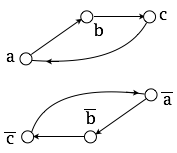
\includegraphics[width=0.3\textwidth]{FiguresGraph/2SATyes.png}
\caption{A portion of the digraph $\g(\Phi_1)$.  The graph's two
  strong components provide a truth assignment for $\Phi_1$: $t(x_1) =
  \mbox{\sc false}$; $t(x_2) = \mbox{\sc false}$; $t(x_3) = \mbox{\sc
    true}$.}
\label{2SATyes}
\end{center}
\end{figure}

\item
Fig.~\ref{2SATno} illustrates $\g(\Phi_2)$, for the formula
\[ \Phi_2 \ = \ (\bar{x}_{3} \vee \bar{x}_{1}) \ \wedge \                                      
(\bar{x}_{1} \vee x_{3}) \ \wedge \ (x_{2} \vee x_{3})
\]
Because the graph contains a (directed) path from vertex $x_1$ to
vertex $\bar{x}_1$, Proposition~\ref{prop:2SAT} assures us that formula
$\Phi_2$ does not admit any satisfying truth-assignment.
\begin{figure}[h]
\begin{center}
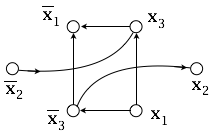
\includegraphics[width=0.3\textwidth]{FiguresGraph/2SATno.png}
\caption{A portion of the digraph $\g(\Phi_2)$.  Because the graph
  contains  a path from vertex $x_1$ to vertex $\bar{x}_1$,  formula
  $\Phi_2$ does not admit any satisfying truth-assignment.}
\label{2SATno}
\end{center}
\end{figure}
\end{enumerate}

\medskip

Even without formal background in algorithmics, it is clear that the
processes of: constructing digraph $\g(\Phi)$ from formula $\Phi$;
isolating and investigating the strongly connected components of
$\g(\Phi)$ can be accomplished in a number of computational steps that
is polynomial in the size of $\Phi$.  This validates
Proposition~\ref{prop:2SAT}.  \qed



\subsubsection{Distance-related concepts}

\noindent {\it Distance and diameter in a digraph.}
\index{digraph!distance between two nodes}
Extrapolating from our discussion of path (\ref{eq:di-path}): The {\it
  distance} from node $u_1$ to node $u_n$ in the digraph $\g$ is the
smallest number of arcs in any path from $u_1$ to $u_n$.  In detail:
\begin{equation}
\label{eq:di-distance-defn}
 \mbox{\sc distance}(u_1, u_n) \ \ \left\{
\begin{array}{cll}
= & 0 & \mbox{  if  } \ u_1 = u_n \\
\leq & n-1 & \mbox{  if there is a path } \ (\ref{eq:di-path})
\ \mbox{ from $u_1$ to $u_n$} \\
= & \infty & \mbox{  if there is no path } \ (\ref{eq:di-path})
\ \mbox{ from $u_1$ to $u_n$}
\end{array}
\right.
\end{equation}
The {\it diameter} \index{diameter in a digraph}
\index{digraph!diameter} of a directed graph $\g$ is the largest
distance between two nodes of $\g$, i.e., the largest number $d$ for
which there exist nodes $u_1, u_n \in \n$ such that {\sc
  distance}$(u_1, u_n) = d$.  Note that when discussing digraphs, we
always use {\em directed} paths when defining distance.
\medskip

\noindent {\it Distance and diameter in an undirected graph.}
\index{graphs!!distance between two nodes}
\index{diameter in a graph}
Extrapolating from our discussion of path (\ref{eq:undi-path}): The
{\it distance between} node $u_1$ and node $u_n$ in the graph $\g$ is
the smallest number of edges in any path from $u_1$ to $u_n$.  In
detail:
\begin{equation}
\label{eq:distance-defn}
 \mbox{\sc distance}(u, v) \ \ \left\{
\begin{array}{cll}
= & 0 & \mbox{  if  } \ u = v \\
\leq & n-1 & \mbox{  if there is a path } \ (\ref{eq:di-path})
\ \mbox{ between $u$ and $v$} \\
= & \infty & \mbox{  if there is no path } \ (\ref{eq:di-path})
\ \mbox{ between $u$ and $v$}
\end{array}
\right.
\end{equation}

The {\it diameter} \index{diameter in a graph} \index{graphs!diameter}
of an undirected graph is the largest distance between two nodes, 
i.e., the largest number $d$ for which the exist a pair of nodes $u_1,
u_n$ such that {\sc distance}$(u_1, u_n) = d$.  Note that
when discussing undirected graphs, we always use {\em undirected}
paths when defining distance.

\ignore{********
Alternatively, this result can be proved by applying the Fubini's
principle using the adjacency matrix.  The two ways of counting the
non-zero elements are by rows (giving the sum of degrees) and globally.
\bigskip

Now, decompose this sum into even and odd degrees.

$\Sigma_{x \in V} \delta(x) = \Sigma_{x \in V_{even}} \delta(x) +
\Sigma_{x \in V_{odd}} \delta(x)$.

As $\Sigma_{x \in V_{even}} \delta(x)$ is obviously even as the sum of
even numbers, $\Sigma_{x \in V_{odd}} \delta(x)$ should also be even.

Thus, the number of odd vertices is even.% as depicted in Figure~\ref{propertyOdd}.
*************}

\bigskip
\noindent \fbox{
\begin{minipage}{0.95\textwidth}
Our discussion of internode distances within graphs have focused on
shortest (or longest) path problems in {\em unweighted} graphs.  A
variety of important applications can be modeled via path-distance
problems in graphs $\g$ each of whose edges, say, $\{u,v\}$, is
weighted with a number that measures the cost of going between nodes
$u$ and $v$ in $\g$.  Of course, when graph $\g$ is directed, then the
arcs $(u \rightarrow v)$ and $(v \rightarrow u)$ can have different
weights, to model situations wherein going from $u$ to $v$ is
easier/cheaper than going from $v$ to $u$.  Happily, determining
shortest (or longest) paths in a directed or undirected graph $\g$ can
be accomplished ``efficiently''---which in the algorithmic world means
``in a number of steps that is polynomial in the size of $\g$''.
\end{minipage}
}

%%%%%%%%%%%%%%%%%%%%%%%%%%%%%%%%%%%%

\subsubsection{Matchings in graphs}
\index{graphs!matching}

The notion of a {\it matching} in a graph is fundamental to many
situations that can be modeled using graphs.  A {\it matching} in an
undirected graph $\g$ is a set of edges of $\g$ that have no nodes in
common.  It is, thus, a formal mechanism for pairing nodes of a graph.
The broad array of activities that can be modeled using graph matching
include: pairing competitors for a tennis tournament; helping a person
select a potential spouse (which even in the vernacular is often
termed ``matchmaking''); determining (near-)optimal layouts for a
keyboard in language X (based on the relative ``affinities'' of
various pars of letters for one another in language X); selecting
persons to command the police stations in city Y (based on the
perceived ``match'' between a candidate's qualifications and the needs
of specific stations).  Even this small sampler of situations that
involve matchings makes it clear that there are many variations on
this formal theme.  This section is devoted to describing, and briefly
discussing, a few of the most commonly encountered versions of
matching in graphs.
\bigskip

\noindent \fbox{
\begin{minipage}{0.95\textwidth}
Although the definitions of the various versions of matching are
readily accessible to even the beginning student of mathematics, much
of the more sophisticated mathematical knowledge about matchings is
beyond any beginning text.  The interested reader might consult a more
advanced source, such as \cite{Berge73}, to get a feeling for what is
known about this simple, yet rich, topic.
\end{minipage}
}
\bigskip

\noindent {\it Matchings in unweighted graphs}.
The most straightforward notion of matching involves an undirected
graph $\g$ with unlabeled edges.  The optimization criterion most
often invoked with this genre of matching is to maximize the number of
edges of $\g$ that belong to the matching.

The target in this ``vanilla-flavored'' matching problem is often a
matching that is {\em maximal}, \index{graphs!maximal matching}
\index{graphs!maximal matching!unweighted graph} in the sense that
adding any further edge of $\g$ to the matching leaves one with a set
of edges that is no longer a matching.

Among maximal matchings in a graph $\g$, the ``ultimate treasure'' is
a matching that is {\it perfect}, \index{graphs!perfect matching} in
the sense that every node of $\g$ belongs to some edge of the
matching.

\begin{prop}
\label{thm:max-matching}
Maximal matchings exist for any graph $\g$.  One can find such a
matching in a number of steps proportional to $|\n|$.
\end{prop}

\begin{proof}
We leave to the reader the challenge of verifying that the following
\index{greedy algorithm} {\em greedy}\footnote{In the world of
  algorithmics, the term ``greedy'' describes any process that seeks to
  satisfy a criterion as quickly as possible, with no consideration of
  how this choice affects future choices.}~process satisfies the
conditions of the Proposition.
\medskip

\noindent
{\it The Process:} \\
Begin by laying the nodes of $\g$ out, left to right, in any way.

\noindent
Repeat the following process until no nodes remain in the layout.

\noindent
Select the leftmost node, $u$, in the remaining layout of $\n$.
%Select the leftmost neighbor, $v$, of $u$ that remains in the layout.
  \begin{itemize}
  \item
If we succeed in finding such a vertex $v$ neighbor of $u$ (taken from left to right)), 
then add edge $\{u,v\}$ to
the matching we are building.  
Then, remove both $u$ and $v$ from the layout.
  \item
If there is no neighbor $v$ of $u$, remove node $u$ from the layout.
  \end{itemize}
The real challenge here is to find a data structure that allows an
efficient search for a ``remaining'' neighbor-node $v$ at each step of
the selection process.
\qed
\end{proof}

\medskip

In contrast to maximal matchings, there exist myriad simple graphs
that do not admit any perfect matching.  Contemplating, for instance,
matchings within any cycle with an odd number of nodes may prepare the
reader for the challenge of verifying the following necessary
condition for a graph to admit a perfect matching.

\begin{prop}
\label{thm:necessary-for-perfect-matching}
Let $\g$ be a graph that admits a perfect matching.  Then:
\begin{itemize}
\item
$\g$ has an even number of nodes.
\item
The cardinality of the (perfect) matching---i.e., the number of edges
in the matching---is exactly
$\frac{1}{2}|\n|$.
\end{itemize}
\end{prop}


\bigskip

\noindent {\it Matchings in weighted graphs}.
The other very popular genre of matching problem focuses on graphs
each of whose edges, say, $\{u,v\}$, is weighted with a number that
measure the ``affinity'' of  nodes $u$ and $v$ for each other.  The
challenge is to find a matching that is {\em maximal}
\index{graphs!maximal matching} in the sense of having a cumulative
sum of edge-weights that is not exceeded by any other matching's.

We note in closing that, while edge-weightings often complicate
computational processing of graphs, they need not render such
computations practically infeasible.  For instance, the problem of
discovering a perfect matching of minimal weight in an edge-weighted
graph can be solved moderately efficiently---i.e., in a number of
steps that is polynomial in the size of the graph.  (An algorithm that
achieves this efficiency can be based on the colorfully named {\it
  Hungarian assignment method}; \index{Kuhn, Harold W.}  see the
original source \cite{Kuhn55} or the encyclopedic algorithms text
\cite{CLRS}.)



%%%%%%%%%%%%%%%%%%%%%%%%%%%%%%%%%

\subsection{Trees}
\label{sec:Trees}

The special class of graphs called {\it trees} \index{graphs!trees}
\index{trees} occupy a place of honor within both the mathematical
field called {\it graph theory} and within the vernacular.
They are identified mathematically as graphs that contain no
cycles or, equivalently, as graphs in which each pair of nodes is
connected by a unique path: a tree is thus the embodiment of ``pure''
connectivity (see Fig.~\ref{fig:tree} left for an example of tree).  As one
would expect from the vernacular, a set of trees is called a {\it
  forest}. \index{forest (of trees)}
\begin{figure}[hbt]
\begin{center}
       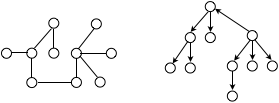
\includegraphics[scale=0.6]{FiguresGraph/tree}
       \caption{An undirected tree with 10 vertices (left) and a directed outtree (right).
       Its root is on the right upper side of the figure.}
  \label{fig:tree}
\end{center}
\end{figure}

Mathematically speaking, a tree is a graph that contains no cycles,
i.e., is {\it cycle-free}. \index{graphs!cycle-free} Equivalently, a
tree is a graph in which each pair of distinct nodes is connected by
precisely one path.  A tree is thus the embodiment of ``pure''
connectivity: it provides the minimal interconnection structure that
provides paths that connect every pair of nodes.  As one might expect
from the vernacular, a set of trees is called a {\it forest}. \index{forest (of trees)}

We have just given two distinct definitions of ``tree''.  The reader
should prove that both definitions define the same class of graphs.

\begin{prop}
\label{thm:2defns-trees}
Prove that the two definitions of ``tree'' are equivalent.  In other
words, prove that the following assertions about a connected graph
$\t$ are equivalent, in the sense that one assertion holds if, and
only if, the other does.
\begin{enumerate}
\item
The graph $\t$ is cycle-free.
\item
Each pair of distinct nodes of $\t$ is connected by precisely one
path.
\item
An $n$-node connected tree $\t$ has precisely $n-1$ edges.
\end{enumerate}
\end{prop}

Let us detail the proof of the last property.

\begin{proof}
\noindent 
Let us proceed by induction on $n$.

The base case $n=2$ is obvious, because one edge is both necessary and
sufficient to connect two nodes.

Assume for induction that the indicated tally is correct for all trees
having no more than $k$ nodes.

Consider, for the purpose of extending the induction, any tree $\t$ on
$k+1$ nodes.  Easily, $\t$ must contain at least one leaf-node---i.e.,
a node $v$ of degree $1$---or else $\t$ would contain a cycle.  If we
remove $v$ and its incident edge, we now have a tree on $k$ nodes
which, by induction, has $k-1$ edges.  When we reattach node $v$, to
restore $\t$ to its original state, we see that $\t$ has $k+1$ nodes
and $k$ edges.

Because $\t$ was an arbitrary $(k+1)$-node tree, the induction is
extended.  \qed
\end{proof}

\bigskip

\noindent \fbox{
\begin{minipage}{0.95\textwidth}
Sociologically, the historical {\it atomic family tree} \index{family
  tree} has two roots, representing the matriarch and patriarch of the
family.  The entirety of the tree represents a single family
generationally, before any children form their own families.  All
child-nodes in this genre of tree are the roots of singly-rooted
subtrees of the entire family tree.  The leaves of the tree are the
childless descendants of the roots.  Note that, while we are using
anthropomorphic language here, we could be discussing other genres of
``family'', as, e.g., many types of biological taxonomies.
\end{minipage}
}
\bigskip

Among rooted directed trees, an important subclass comprises those
that have a {\em single root} which has a directed path to every other
node.  The length of each such directed path is often used to label
the {\it generation}
\index{generation of a node in a singly-rooted directed tree}
of the node at the end of the path: root, child, grandchild,
great-grandchild, etc.
Every node of the tree is the root of a singly-rooted directed
subtree of the entire tree.  All subtrees that are rooted at nodes of
the same generation are mutually disjoint.
\bigskip

\noindent \fbox{
\begin{minipage}{0.95\textwidth}
A singly-rooted tree represents a {\it hierarchy}.
\index{trees!singly-rooted!hierarchy} \index{hierarchy} Given two
directed subtrees within a hierarchy, either the root of one of the
subtrees is a descendant of the root of the other, or the two subtrees
are are mutually disjoint.
\end{minipage}
}
\bigskip

More formally: {\em rooted trees} are a class of {\em acyclic}
digraphs.  Paths in trees which start at the root are often called
{\em branches}.  The {\em acyclicity} of a tree $\t$ means that for
any branch of $\t$ of the form (\ref{eq:di-path}), we cannot have $u_1
= u_n$, for this would create a cycle.  Each singly-rooted tree $\t$
has a designated {\em root node} \index{trees!root node} $u_n \in
\n_{\ft}$ that resides at the end of a branch (\ref{eq:di-path}) that
starts at $r_{\ft}$ (so $u_1 = r_{\ft}$) is said to reside at {\em
  depth} $n-1$ in $\t$; by convention, $r_{\ft}$ is said to reside at
depth $0$.  \index{depth of a node in a singly-rooted trees} $\t$'s
root $r_{\ft}$ has some number (possibly $0$) of arcs that go from
$r_{\ft}$ to its {\em children,} each of which thus resides at depth
$1$ in $\t$; in turn, each child has some number of arcs (possibly
$0$) to its children, and so on.  For each arc $(u \rightarrow v) \in
A_{\ft}$, we call $u$ a {\it parent} \index{trees!parent node} of $v$,
and $v$ a {\it child} \index{trees!child node} of $u$, in $\t$;
clearly, the depth of each child is one greater than the depth of its
parent.  Every node of $\t$ except for $r_{\ft}$ has precisely one
parent; $r_{\ft}$ has no parents.  A childless node of a tree is a
{\em leaf}, \index{trees!leaf node} i.e., a node of degree $1$.  The
transitive extensions of the parent and child relations are,
respectively, the {\em ancestor} \index{trees!ancestor node} and {\em
  descendant} \index{trees!descendant node} relations.  The {\em
  degree} \index{degree (of a node in a tree)} of a node $v$ in a tree
is the number of children that the node has, call it $c_v$.  If every
non-leaf node in a tree has the same degree $c$, then we call $c$ the
{\em degree of the tree}.  \index{degree of a tree}

It is sometimes useful to have a symbolic notation for the ancestor
and descendant relations.  To this end, we write $(u \Rightarrow v)$
\index{$\Rightarrow$: ancestor/descendant in a rooted tree} to
indicate that node $u$ is an {\it ancestor} of node $v$, or
equivalently, that node $v$ is a {\it descendant} of node $u$.  If we
decide that we are not interested in {\em really distant} descendants
of the root of a tree $\t$, then we can {\em truncate} \index{truncated}
$\t$ at a desired depth $d$ by removing all nodes whose depths exceed
$d$.  We thereby obtain the {\em depth-$d$ prefix} of $\t$.

\ignore{****************
Figure \ref{fig.graph-samples} depicts an arc-labeled rooted tree $\t$
whose arc labels come from the alphabet $\{a,b\}$.  $\t$'s arc-induced
relationships are listed in Table~\ref{tab.graph-samples}.
\begin{figure}[htb]
\centerline{\epsfig{figure=graph.sample.eps,height=4truecm}}
\caption{An arc-labeled rooted tree $\t$ whose arc labels come from
  the alphabet $\{a,b\}$.  (Arc labels have no meaning; they are just
  for illustration.)
\label{fig.graph-samples}}
\end{figure}
\begin{table}[htb]
{\small
\begin{center}
\fbox{
\begin{tabular}{c||c|c|c|c}
\multicolumn{5}{c}{The arc-labeled rooted tree $\t$ of
  Figure \ref{fig.graph-samples}} \\
\hline
Node            & Children & Parent & Descendants & Ancestors \\
\hline
\hline
$r_{\ft} = u_0$ 
& $u_1$
& none & 
$u_1, u_2, \ldots, u_k, v_1, v_2, \ldots, v_k,
w_1, w_2, \ldots, w_k$
& none \\
\hline
$u_1$
& $u_2, v_1$
& $u_0$ & 
$u_2, \ldots, u_k, v_1, v_2, \ldots, v_k, w_1, w_2, \ldots, w_k$
& $u_0$ \\
\hline
$u_2$
& $u_3, v_2$
& $u_1$ & 
$u_3, \ldots, u_k, v_2, \ldots, v_k, w_2, \ldots, w_k$
& $u_0$ \\
\hline
 $\vdots$ & $\vdots$ & $\vdots$ &  $\vdots$ &  $\vdots$ \\
\hline
$u_k$
& $v_k$ 
& $u_{k-1}$ & 
$v_k, w_k$
& $u_0, u_1, \ldots, u_{k-1}$ \\
\hline
$v_1$
& $w_1$ 
& $u_1$ & 
$w_1$
& $u_0, u_1$ \\
\hline
$v_2$
& $w_2$
& $u_2$ & 
$w_2$
& $u_0, u_1, u_2$ \\
\hline
 $\vdots$ & $\vdots$ & $\vdots$ &  $\vdots$ &  $\vdots$ \\
\hline
$v_k$
& $w_k$
& $u_k$ & 
$w_k$
& $u_0, u_1, \ldots, u_k$ \\
\hline
$w_1$
& none
& $v_1$ & 
none
& $u_0, u_1, v_1$ \\
\hline
$w_2$
& none &
$v_2$ & 
none
& $u_0, u_1, u_2, v_2$ \\
\hline
$w_k$
& none
& $v_k$ & 
none
& $u_0, u_1, \ldots, u_k, v_k$
\end{tabular}
}
\end{center}
}
\caption{A tabular description of the rooted tree $\t$ of
  Figure \ref{fig.graph-samples}.  \label{tab.graph-samples}}
\end{table}
*********************}

\subsubsection{Spanning trees}

One of the major uses of trees and forests is as a way of succinctly
``summarizing'' the connectivity structure inherent in an undirected
graph.  This role is inherent in the notion of a {\it spanning tree}
\index{graphs!spanning tree} \index{spanning tree} of a connected
graph $\g$.  A spanning tree of $\g$ is a tree $\t(\g)$ whose node-set
is identical to $\g$'s:
\[ \n_{\ft(\fg)} \ = \ \n_{\fg} \]
and all of whose edges are edges of $\g$:
\[ \e_{\ft(\fg)} \ \subseteq \ \e_{\fg}. \]
Not surprisingly, a connected graph $\g$  typically has {\em many}
spanning trees.  All such trees share $\g$'s node-set, but they may
choose quite different sets of edges.

\ignore{
{\Arny Chance for some exercises here}

For a graph $\g$ that is not connected, we replace the notion of
spanning tree of $\g$ with the analogous notion of a {\it spanning
  forest} \index{graphs!spanning forest} \index{spanning forest} of
$\g$.  We shall typically discuss only spanning trees in this section,
leaving the reader to extrapolate the discussion to include spanning
forests of unconnected graphs.
}


The major use of spanning trees in applications is to ``summarize''
the full connectivity structure of a graph---and of the entities that
the graph models, such as a map, the layout of a museum, etc.  When
used in this way, the edges of spanning trees are typically {\em
  weighted}, \index{graphs!spanning tree!edge-weighted} in order to
model a ``cost'' of incorporating that edge in the tree.  The types of
computational problem modeled via edge-weighted spanning trees
include: the optimal placement of firehouses, or hospitals, in a town
and the optimal deployment of security mechanisms in an art museum.
Reflecting problems wherein edge-weights measure transit costs, it is
a classical computational problem to seek a {\em minimum-weight
  spanning tree} \index{graphs!minimum-weight spanning tree}
\index{minimum-weight spanning tree} (or, in the vernacular, a {\em
  minimum spanning tree}).  Happily, this classical optimization
problem can be solved within a number of steps that is linear in the
number of edges of $\g$ \cite{CLRS}.

\ignore{
I put in the exercice session
{\Arny Giving just a {\em hint} at a solution for MST to real
  beginners is probably useless}

There are mainly two ways for constructing such a MST, each one
emphasizes a different propriety of the MST, namely, avoid cycles and
minimize the span.  In both cases, the edges are sorted in increasing
order of weights.  More precisely, the first one constructs a subtree
which partially spans the graph by adding at each step the minimum
neighboring edge while the other add successively the edges of minimal
weights that do not create a cycle.
}

Just as with graphs, there is a {\em directed} version of trees which
is formed by replacing the (unoriented) edges of an undirected tree by
(oriented) arcs; see the right side of Fig.~\ref{fig:tree}.  Within a directed tree
$\t$, one often says that an arc goes from a {\it parent node}
\index{trees!parent node} to a {\it child node} \index{trees!child
  node}.  Extending this anthropomorphic metaphor, one often talks
about the {\it ancestor(s)} \index{trees!ancestor node} and {\it
  descendant(s)} \index{trees!descendant node} of a tree-node.  We
single out two special classes of nodes: A {\it root (node)}
\index{trees!root (node)} \index{root (of a directed tree)} of $\t$ is
defined by its having no entering arcs, i.e., indegree $0$; a {\it
  leaf (node)} \index{trees!leaf (node)} \index{leaf (of a directed
  tree)} of $\t$ is defined by its having no exiting arcs, i.e.,
outdegree $0$.  The reader is certainly familiar with the use of
rooted directed trees to represent family trees and corporate
hierarchies.

%%%%%%%%%%%%%%%%%%%%%%%%%%%%%%%%%%%

\subsection{Computationally Significant ``Named'' Graphs}
\label{sec:graphs-important-families}

The mathematical discipline called graph theory is an important source
of formal aids for the activities of designing, analyzing, utilizing,
and verifying computer systems.  Of course, computer systems are
designed by humans.  Among other consequences of this fact is the
observations that the graphs that are among the most commonly used to
structure systems tend to be rather uniform in structure, in a variety
of possible ways.  Such graphs, when drawn, often exhibit a lot of
structural symmetry.  One popular form of symmetry is {\it degree
  regularity}: an undirected graph $\g$ is {\it regular}
\index{graphs!regular} if all nodes of $\g$ have the same degree.  Not
surprisingly, there is a directed version of ``regular'' embodied in the
symmetric notions of {\it in-regularity}
\index{graphs!directed!in-regular} and {\it out-regularity}.
\index{graphs!directed!out-regular}

\medskip

We now describe five families of regular graphs that have proven
useful over the history of digital computing, and we expose some basic
properties of each, including its diameter.  Each of these graphs is
available in both a directed and an undirected version, although, as
we note, one of these versions is more commonly encountered.  We have
selected these specific graphs for rather different reasons.
\begin{itemize}
\item
The first two graphs, the {\it cycle-graph} of section~\ref{sec:cycle}
and the {\it complete graph} of section~\ref{sec:clique} were selected
for respectively representing the lowest-degree and highest-degree
graphs that share two properties: (1) every node of each graph is
accessible from every other node; (2) all nodes ``look alike'' to
someone traversing the graph.  Elaborating on (2): If we put you down
on a node of either graph, there is no way that you can determine the
identity of that node.  This is an important feature to ponder,
because it is a simple instance of the anonymity problem inherent to
many modern distributed computing environments.  {\it How does one
  orchestrate cooperative activities when all agents ``are
  identical''?}
\item
The remaining graphs, the {\it mesh and torus networks}\footnote{These
  two structures, though distinct, are usually discussed together
  because they share so many important properties.}~of section~\ref{sec:mesh}, 
  the {\it hypercube network} of section~\ref{sec:hypercube},
and the {\it de Bruijn network} of section~\ref{sec:deBruijn}, were
selected for their importance within the world of parallel and
distributed computing---as abstract platforms for developing efficient
computational and communicational processes, and as abstract versions
of the networks that underlie parallel architectures by
interconnecting its processors.
\end{itemize}
Throughout, the parameters that describe our graph families range over
the positive integers; i.e., each occurrence of $n$ below ranges over
$\N^+$.

\subsubsection{The cycle-graph $\cc_n$}
\label{sec:cycle}

{\Denis The notation with a hat for the directed version is not the same as
the reverse graph presented before. Do we really need to present the reverse graph???}

For each positive integer $n \in \N^+$, both the {\it undirected
  order-$n$ cycle-graph} $\cc_n$ and the {\it directed order-$n$
  cycle-graph} $\widehat{\cc}_n$ \index{cycle graph} \index{cycle
  network} have {\it node-set}
\[ \n_{{\cal C}_n} \ = \ \n_{\widehat{{\cal C}}_n}
\ = \ \{ 0, \ 1, \ \ldots, \ n-1\}. \]
\begin{itemize}
\item
$\cc_n$ has $n$ edges; its {\it edge-set} is
\[ \e_{{\cal C}_n} \ = \
\big\{ \{i, \ i+1 \bmod n\} \ \ | \ \ i \in \{0, \ 1, \ \ldots,
\ n-1\} \big\}.
\]
Fig.~\ref{fig:cycle} illustrates a cycle with $8$ vertices.
  \begin{itemize}
  \item \index{cycle graph!node-degree}
$\cc_n$ is a regular network: each node has degree $2$.

Specifically, each node $i$ of $\cc_n$ has its {\it predecessor} $i-1
\bmod n$ \index{cycle graph!predecessor node} \index{cycle
  graph!successor node} and its {\it successor} $i+1 \bmod n$ .
  \item \index{cycle graph!diameter}
$\cc_n$ has diameter $\lfloor n/2 \rfloor$.

Direct calculation shows that $\cc_n$'s diameter is no larger than
this.  The fact that this is, in fact, the graphs's diameter is
witnessed by the distance between each node $k \in \n_{{\cal C}_n}$
and its antipodal node $k + \lfloor n/2 \rfloor \bmod n$.
  \end{itemize}

\item
$\widehat{\cc}_n$ has {\it arc-set}
\[ \a_{\widehat{{\cal C}}_n} \ = \ 
\big\{ (i \rightarrow i+1 \bmod n) \ \ | \ \ i \in \{0, \ 1, \ \ldots, \ n-1\} \big\}
\]
  \begin{itemize}
  \item \index{cycle graph!directed node-degree}
$\widehat{\cc}_n$ is a regular network: each node has the same
    indegree and the same outdegree.  Coincidentally, both the common
    indegree and the common outdegree are $2$.
  \item
$\widehat{\cc}_n$ has (directed) diameter $n-1$.

Of course, $n-1$ is an upper bound on the diameter of any $n$-node
digraph.  The fact that this is exactly the graph's diameter is
witnessed by the directed distance from each node $k$ of $\widehat
{\cc}_n$ to its predecessor node $k-1 \bmod n$.
  \end{itemize}
\end{itemize}

\begin{figure}[hbt]
\begin{center}
       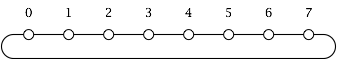
\includegraphics[scale=0.6]{FiguresGraph/cycle}
       \caption{A cycle of $8$ vertices.}
  \label{fig:cycle}
\end{center}
\end{figure}

\subsubsection{The complete graph, or, clique $\k_n$}
\label{sec:clique}
\index{complete graph} \index{clique}

For each positive integer $n \in \N^+$, we denote by $\k_n$ the {\em
  undirected} order-$n$ {\it complete-graph} (or, {\it clique}),
\index{complete graph} \index{clique} and by $\widehat{\k}_n$ the {\em
  directed} order-$n$ {\it complete-graph} (or, {\it clique}).  Both
$\k_n$ and $\widehat{\k}_n$ have {\it node-set}
\[ \n_{{\cal K}_n} \ = \ \n_{\widehat{{\cal K}}_n}
\ = \ \{ 0, \ 1, \ \ldots, \ n-1\}. \]
\begin{itemize}
\item
$\k_n$ has $\displaystyle {n \choose 2}$ edges; its {\it edge-set} is
\[ \e_{{\cal K}_n} \ = \
\big\{ \{i, \ j\} \ \ | \ \ i,j \in \{0, \ 1, \ \ldots, \ n-1\}, \ i
\neq j \big\}.
\]
  \begin{itemize}
  \item \index{complete graph!node-degrees} \index{clique!node-degrees}
$\k_n$ is a regular network: each node has degree $n-1$; every node $i
\in \n_{\fk_n}$ is connected with all other nodes.

   \item \index{complete graph!diameter}
$\k_n$ has diameter $1$.

$\k_n$'s diameter is a direct consequence of its node-degrees, and vice versa.
  \end{itemize}

\item
$\widehat{\k}_n$ has $(n-1)n$ arcs; its {\it arc-set} is
\[ \a_{\widehat{{\cal K}}_n} \ = \ 
\big\{ (i \rightarrow j) \ \ | \ \ i,j \in \{0, \ 1, \ \ldots, \ n-1\}
\big\}, \ i \neq j
\]
  \begin{itemize}
  \item
$\widehat{\k}_n$ is a regular network: each node has the same indegree
    and the same outdegree.  Both the common indegree and the common
    outdegree are $n-1$.
  \item
$\widehat{\k}_n$ has (directed) diameter $1$.

As in the undirected case, there is a causal relationship between
$\widehat{\k}_n$'s diameter and its (in- and out-) node-degrees.
  \end{itemize}
\end{itemize}

{\Denis good opportunity for an exercice here: a tournoiment 
is a directed version of a complete graph (any orientation of the edges).
The proof that it is hamiltonian is nice, If you agree I can add it in the exercices...}

Hearkening back to our discussion of matchings in (unweighted) graphs:
The structure of the set of perfect matchings in general graphs is
decidely nontrivial.  For clique-graphs, though, the structure is much
easier to discuss.

\begin{prop}
\label{thm:perfect-matchings-clique}
The number of perfect matchings admitted by the clique-graph $\k_n$ is
either $0$---if $n$ is odd---or exponential in $n$ if $n$ is even.
\end{prop}

\begin{proof}
The assertion about cliques with odd numbers of nodes is immediate
from Proposition~\ref{thm:necessary-for-perfect-matching}.

We verify the assertion about cliques of the form $\k_{2k}$ by
induction on $k$.  To this end, let $M_n$ denote the number of perfect
matchings that the clique $\k_n$ admits.

The base of our induction is the case $k=1$.  Because $\k_{2}$
consists of a single edge, it admits only one perfect matching; i.e.,
$M_1 = 1$.
%(see Figure~\ref{perfectMatching1}): 

To garner intuition, we also explicitly solve the case $k=2$, which is
illustrated in Fig.~\ref{fig:AllPerfectMatchings}.
\begin{figure}[hbt]
\begin{center}
       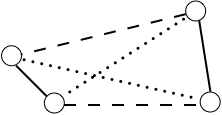
\includegraphics[scale=0.55]{FiguresGraph/perfectmatchingAll}
       \caption{The $4$-nodes clique graph  $\k_4$ (left) and its three different perfect matchings (right): 
       the matchings' edges are drawn, respectively, with bold lines, dashed lines, and dotted lines.}
%of one matching are drawn in bold;
% The optimal one is represented in bold (the two others are in dashed and dot lines).}
  \label{fig:AllPerfectMatchings}
\end{center}
\end{figure}
As the figure illustrates, $\k_4 = \k_{2 \cdot 2}$ can be viewed as a
$4$-cycle (drawn with bold and dashed lines), augmented by two
``cross-edges'' (drawn with dotted lines).  Easily, then, $\k_4$
admits $3$ different perfect matchings, which can be identified (and
specified) by the edge that contains the northwesterly node---call it
$v$---in the figure.  Node $v$ has the choice of three nodes to
``boldly'' match with. (In the figure, $v$ has chosen the
southwesterly node as its ``bold'' match.)  Once $v$ has chosen its
match, there is only one viable choice for the second edge in the
matching.  Thus, $M_2=3$.

We jump now to the case of any arbitrary $k > 2$.  We remark that
there are precisely $2k-1$ nodes of $\k_{2k}$ that node $1$ can
``choose'' as its mate in a perfect matching.  Once we set node $1$
and its chosen mate aside, we confront an independent instance of the
problem with parameter $k-1$, i.e., the problem of counting the number
of perfect matchings in $\k_{n-2} = \k_{2k-2}$.  We thereby note that
as $k$ grows, the quantity $M_k$ obeys the following recurrence:
\[ M_k \ = \ (2k-1) \cdot M_{k-1} \]
In other words:

\hspace*{.25in}{\em $M_k$ is the product of the first $k$ odd numbers.}
%$N_1=1$, $N_2=3$, $N_3=3 \times 5=15$, $N_4=3 \times 5 \times 7=115$, etc..

\noindent
To gauge the growth rate of $M_k$, we concentrate on cases $k > 2$ and
ignore the $\lfloor k/2 \rfloor$ smallest odd numbers.  We then
replace each of the remaining odd numbers by its smallest possible
value.  We thereby find that
\[
M_k \ \ =    \ \ \prod_{i=1}^k \ (2i-1)
    \ \ \geq \ \ \prod_{\lceil k/2 \rceil}^k \ (2i-1)
    \ \ \geq \ \ \left( 2 \lceil k/2 \rceil -1 \right)^{k/2}
    \ \ >    \ \ k^{k/2}
\]
In summary, $M_k$ grows exponentially with the parameter $k$, as claimed.
\qed
\end{proof}


\bigskip

The two families of graphs we have just discussed, cycles and cliques,
are recommended to our attention by their structural simplicity---they
epitomize, respectively, the most sparse way (the cycle) and the most
dense way (the clique) to completely interconnect $n$ nodes.  The
remainder of this section is devoted to three graph-structures that
are structurally more complex than cycles and cliques, which have been
designed to meet specific needs within the real technological world of
computing and communicating.  Indeed, the three upcoming graph
families are among the most important ones when discussing parallel
and distributed computing (PDC, for short).  All three families have
been used both to design computer architectures that support PDC and
to craft algorithms that exploit the potential efficiencies---in
computation and communication---that one can achieve using PDC.

\subsubsection{The mesh ($\m_{m,n}$) and torus ($\widetilde{\m}_{m,n}$) networks}
\label{sec:mesh}
\index{mesh and torus networks}

For positive integers $m, n \in \N^+$, both the $m \times n$ {\it mesh
  (network)} $\m_{m,n}$ and the $m \times n$ {\it toroidal network}
(or, {\it torus}) $\widetilde{\m}_{m,n}$ have {\it node-set}
\begin{eqnarray*}
\n_{\fm_{m,n}} \ = \ \n_{\widetilde{\fm}_{m,n}}
  & = & 
\{1, \ 2, \ldots, \ m\} \ \times \ \{1, \ 2, \ldots, \ n\} \\
  & = & 
\big\{ \langle i, \ j \rangle \ \ | \ \ 
\big[ i \in \{1, \ 2, \ldots, \ m\} \big], \ \
\big[ j \in \{1, \ 2, \ldots, \ n\} \big]
\big\}
\end{eqnarray*}

\begin{itemize}
\item
$\m_{m,n}$ has $(m-1)n \ + \ (n-1)m$ edges; its {\it edge-set} is
\begin{eqnarray*}
\e_{\fm_{m,n}} & = & 
\big\{
\{ \{ i, j \}, \ \{ i+1, j \} \ \ | \ \
1 \leq i < m, \ \ 1 \leq j \leq n \} \\
  &  & \hspace*{.1in} \cup
\{ \{ i, j \}, \ \{ i, j+1 \} \ \ | \ \
1 \leq i \leq m, \ \ 1 \leq j < n \}
\big\}
\end{eqnarray*}

{\Denis I removed the formal definitions of corners, edges
since I don't see what this really add to the text (we don't use this later),
let discuss if you disagree... }

\begin{itemize}
\item
The subgraph of $\m_{m,n}$ defined by the node-set
\[ \{ \langle i, \ j \rangle  \ \ | \ \ \left[i \in \{1, 2, \ldots,
  m\}\right], \ \ \left[1 \leq j < n\right]\}
\]
{\Denis Definition not clear: for me, $i$ should be fixed, and then, $j$ varies}
and all edges both of whose endpoints belong to that set is called the
$i$th {\it row} of $\m_{m,n}$
\index{row of a mesh graph}
\index{mesh graph!row}
Dually, the subgraph of $\m_{m,n}$ defined by the node-set
\[ \{ \langle i, \ j \rangle  \ \ | \ \ \left[j \in \{1, 2, \ldots,
  n\}\right], \ \ \left[1 \leq i < m\right] \}
\]
and all edges both of whose endpoints belong to that set is called the
$j$th {\it column} of $\m_{m,n}$.
\index{column of a mesh graph}
\index{mesh graph!column}
\ignore{
  \begin{itemize}
     \item
Nodes $\langle 1, \ 1 \rangle$, $\langle 1, \ n \rangle$, $\langle m,
\ 1 \rangle$, and $\langle m, \ n \rangle$ are the {\it corner nodes}
(or, just {\it corners}) of $\m_{m,n}$.
\index{corner (node) of a mesh graph}
\index{mesh graph!corner (node)}
     \item
The path-graph consisting of the node-set
\[ \{ \langle 1, \ 1 \rangle, \ \langle 1, \ 2 \rangle, \ldots, \
\langle 1, \ n \rangle \}
\]
together with all edges of $\m_{m,n}$ both of whose endpoints belong
to this set, is the {\it top edge} of $\m_{m,n}$.
\index{top edge of a mesh graph}
\index{mesh graph!top edge}

The other edges of $\m_n$ are defined analogously:

\smallskip

The {\it bottom edge} of $\m_{m,n}$ is the path-graph built upon the
node-set
\[ \{ \langle m, \ 1 \rangle, \ \langle m, \ 2 \rangle, \ldots, \
\langle m, \ n \rangle \}
\]
\index{bottom edge of a mesh graph}
\index{mesh graph!bottom edge}

The {\it left edge} of $\m_{m,n}$ is the path-graph built upon the
node-set
\[ \{ \langle 1, \ 1 \rangle, \ \langle 2, \ 1 \rangle, \ldots, \
\langle m, \ 1 \rangle \}
\]
\index{left edge of a mesh graph}
\index{mesh graph!left edge}

The {\it right edge} of $\m_{m,n}$ is the path-graph built upon the
node-set
\[ \{ \langle 1, \ n \rangle, \ \langle 2, \ n \rangle, \ldots, \
\langle m, \ n \rangle \}
\]
\index{left edge of a mesh graph}
\index{mesh graph!right edge}
     \end{itemize}
     }

  \item \index{mesh graph!node-degree}
$\m_{m,n}$ is {\em not} a regular graph.  Its four corner nodes each has
    degree $2$; its non-corner extreme edge nodes each has degree $3$; its
\index{internal node of a mesh graph}
\index{mesh graph!internal node}
{\em internal nodes} each has degree $4$

  \item \index{mesh graph!undirected diameter}
The diameter of $\m_{m,n}$ is $m+n-2$, as witnessed by the distance
between nodes $\langle 1, \ 1 \rangle$ and $\langle 2, \ n \rangle$.
  \end{itemize}

\item
$\widetilde{\m}_{m,n}$ has $2mn$ arcs; its {\it arc-set} is
\begin{eqnarray*}
\a_{\widetilde{\m}_{m,n}} & = &
\big\{
\{ (\langle i, \ j \rangle \rightarrow \langle i+1 \bmod m, \ j
\rangle) \ \ | \ \ 1 \leq i \leq m, \ \ 1 \leq j \leq n \} \\
  &  & \hspace*{.1in} \cup
\{ (\langle i, \ j \rangle \rightarrow \langle i, \ j+1 \bmod n
\rangle) \ \ | \ \ 1 \leq i \leq m, \ \ 1 \leq j \leq n \}
\big \}
\end{eqnarray*}

\ignore{
  \begin{itemize}
  \item
The subgraph of $\widetilde{\m}_{m,n}$ defined by the node-set
\[ \{ \langle i, \ j \rangle  \ \ | \ \ \left[i \in \{1, 2, \ldots,
  m\}\right], \ \ \left[1 \leq j \leq n\right]\}
\]
and all edges both of whose endpoints belong to that set is called the
$i$th {\it row} of $\widetilde{\m}_{m,n}$
\index{torus graph!row}
Dually, the subgraph of$\widetilde{\m}_{m,n}$ defined by the node-set
\[ \{ \langle i, \ j \rangle  \ \ | \ \ \left[j \in \{1, 2, \ldots,
  n\}\right], \ \ \left[1 \leq i \leq m\right] \}
\]
and all edges both of whose endpoints belong to that set is called the
$j$th {\it column} of $\widetilde{\m}_{m,n}$.
\index{torus graph!column}
}
\begin{itemize}
  \item
$\widetilde{\m}_{m,n}$ is a regular network; each node has degree $4$.
    Despite the fact that $\widetilde{\m}_{m,n}$ is an {\em
      undirected} graph, its arcs are commonly referred to via an
    anthropomorphic labeling, either as ``up, down, left, and right''
    or as ``north, south, west, and east''.
  \item \index{mesh graph!directed diameter}
$\widetilde{\m}_{m,n}$'s diameter is $\lfloor m/2 \rfloor \ + \
\lfloor n/2 \rfloor$.  This can be verified in analogy to the diameter
of the cycle-graph $\cc_n$.
\end{itemize}
\end{itemize}

\begin{figure}[hbt]
\begin{center}
       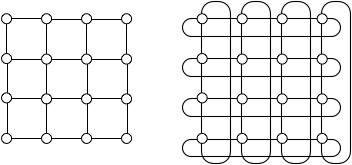
\includegraphics[scale=0.6]{FiguresGraph/meshtorus}
       \caption{$\m_{4,4}$ (left) and $\widetilde{\m}_{4,4}$ (right).}
  \label{fig:torus}
\end{center}
\end{figure}



\subsubsection{The (boolean) hypercube network $\q_n$}
\label{sec:hypercube}
\index{boolean hypercube}
\index{hypercube}

The graphs we focus on in this section have had a major impact on the
world of coding, especially in regard to codes that are {\em error
  correcting} \cite{PetersonW81}, and the world of computing,
especially in regard to parallel and distributed computing
\cite{JohnssonH1989, SaadS89, Schwartz80}.  The cited sources give a
range of perspectives on the importance of {\it hypercube networks.}

\index{order-$n$ boolean hypercube}
The {\it order-$n$ boolean hypercube}, traditionally denoted $\q_n$,
is the $2^n$-node graph defined as follows.
\begin{itemize}
\item
{\it The recursive definition}. 
\index{order-$n$ boolean hypercube!recursive definition}
  \begin{itemize}
  \item
The order-$0$ boolean hypercube, $\q_0$, has a single node, and no
edges.
  \item
The order-$(k+1)$ boolean hypercube, $\q_{k+1}$, is obtained by taking
two copies of $\q_k$, call them $\q_k^{(1)}$ and $\q_k^{(2)}$, and
creating an edge that connects each node of $\q_k^{(1)}$ with the
corresponding node of $\q_k^{(2)}$.
  \end{itemize}
For illustration:
  \begin{itemize}
  \item
$\q_1$ consists of two nodes connected by a single edge.
  \item
$\q_2$ can be viewed as a ``square'', or equivalently, a copy of $\cc_4$.
  \item
$\q_3$ can be viewed as a ``cube'', i.e., as two copies of $\cc_4$
    with edges connecting corresponding nodes: Each of the following
    pairs of nodes are connected by an edge: the upper right
    corner-nodes, the upper left corner-nodes, the lower right
    corner-nodes, and the lower left corner-nodes.
  \end{itemize}

\item
{\it The direct definition}.
For each $n \in \N$, the nodes of the order-$n$ boolean hypercube,
$\q_n$, are all length-$n$ binary strings.  For illustration:
\index{order-$n$ boolean hypercube!direct definition}
\begin{eqnarray*}
\n_{{\fq}_0}
  & = & 
\{ \varepsilon \}, \ \ \mbox{ the length-$0$ {\em null string}} \\ 
\n_{{\fq}_1}
  & = &
\{ 0, \ 1 \} \\
\n_{{\fq}_2}
  & = & \{ 00, \ 01, \ 10, \ 11 \} \\
\n_{{\fq}_3}
  & = & \{ 000, \ 001, \ 010, \ 011, \ 100, \ 101, \ 110, \ 111 \} 
\end{eqnarray*}
The iteration-based construction of big hypercubes from the next
smaller ones is illusrated in Fig.~\ref{fig:hypercube}.
\begin{figure}[hbt]
\begin{center}
       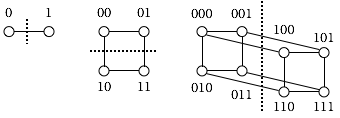
\includegraphics[scale=0.6]{FiguresGraph/hypercube}
\caption{The iteration-based construction of order-$n$ hypercubes:
  Take two copies of the order-$(n-1)$ hypercube.  Prepend a $0$ to
  the node-labels of the first copy and a $1$ to the node-labels of
  the second copy.}
  \label{fig:hypercube}
\end{center}
\end{figure}

Easily, for each value of $n$, $\q_n$ has $2^n$ nodes, for this is the
number of length-$n$ binary strings.

\medskip

For each value of $n$, each edge of $\q_n$ connects two node-strings
that differ in precisely one position.  This means that $\q_n$ has $n
2^{n-1}$ edges: To wit, each of its $2^n$ nodes has $n$ neighbors, so
the quantity $n 2^n$ counts each of $\q_n$'s edges twice---one for
each endpoint.  For illustration:
\begin{eqnarray*}
\e_{{\fq}_1}
  & = &
\big\{ \{ 0, \ 1 \} \big\} \\
\e_{{\fq}_2}
  & = & \big\{
\{ 00, \ 01 \}, \ \{ 00, \ 10\}, \
\{ 01, \ 11 \}, \ \{ 10, \ 11\} 
\big\} \\
\e_{{\fq}_3}
  & = & \big\{ 
\{000, \ 001\}, \
\{000, \ 010\}, \
\{000, \ 100\}, \
\{001, \ 011\}, \\
  &  & \hspace*{.2in}
\{001, \ 101\}, \
\{010, \ 011\}, \
\{010, \ 110\}, \
\{100, \ 101\}, \\
  &  & \hspace*{.2in}
\{100, \ 110\}, \
\{101, \ 111\}, \
\{011, \ 111\}, \
\{110, \ 111\}
\big\}
\end{eqnarray*}
\end{itemize}

\medskip

\noindent
It is easy to observe $\q_n$'s basic structural properties.
\begin{itemize}
\item \index{hypercube!node-degree}
$\q_n$ is a regular network: each of its $2^n$ nodes has degree $n$.

This follows from the fact that each edge of $\q_n$ rewrites a single
bit-position in the length-$n$ binary string that is the edge's source
node.

\item \index{hypercube!diameter}
$\q_n$ has diameter $n \ = \ \ln(|\n_{\fq_n}|)$.\footnote{Recall that
  $\ln n = \log_2 n$; see Section~\ref{sec:logarithmic-fns}.}

We address this issue formally.
\end{itemize}

\begin{prop}
\label{thm:hypercube-diameter}
For all $n \in \N^+$, $\q_n$ has diameter $n \ = \ \ln(|\n_{\fq_n}|)$.
\end{prop}

\begin{proof}
We prove this diameter bound by construction.  Focus on two arbitrary
nodes of $\q_n$:
\[ x \ = \ \alpha_1 \alpha_2 \cdots \alpha_n \ \ \ \mbox{ and } \ \ \
y \ = \ \beta_1 \beta_2 \cdots \beta_n
\]
One of the several paths in $\q_n$ from $x$ to $y$ is described
schematically as the following left-to-right, bit-by-bit rewriting of
$x$ as $y$ using edges of $\q_n$
\[
x \ = \ \alpha_1 \alpha_2 \cdots \alpha_n \ \rightarrow \
\beta_1 \alpha_2 \cdots \alpha_n \ \rightarrow \
\beta_1 \beta_2\cdots \alpha_n \ \rightarrow \cdots \rightarrow\ 
\beta_1 \beta_2 \cdots \beta_n \ = \ y
\]
Since each bit of each string is rewritten at most once (only if $\alpha_i \neq \beta_i$), the bound follows.
\qed
\end{proof}

\medskip

The fact that $\q_n$'s diameter is {\em logarithmic} in its size makes
$\q_n$ an efficient network for many tasks related to parallel
computing and communication.
\bigskip

A powerful avenue for understanding the structure of a given family of
networks is to understand how the perceived ``shape'' of graphs in the
family can apparently change just by relabeling/renaming the nodes, or
the edges, of the graphs.  The formal mechanism for studying such
relabelings/renamings is the concept of {\it graph isomorphism}.
\index{graph isomorphism} Let $\g$ and $\h$ be undirected graphs that
have the same numbers of nodes and edges.  (The following definition
can easily be adapted to deal with {\em directed} graphs.)  An {\it
  isomorphism} between $\g$ and $\h$ is a {\em
  bijection}\footnote{Recall, from Chapter~\ref{ch:sets-BA-logic} that
  a bijection is a function that is one-to-one (i.e., injective) and
  onto (i.e., surjective).}
\[ f: \n_{\fg} \ \leftrightarrow \ \n_{\fh} \]
such that
\begin{itemize}
\item
For each edge $\{ u,v \}$ of $\g$ (i.e., $\{ u,v \} \in \e_{\fg}$),
the doubleton set $\{ f(u), f(v) \}$ is an edge of $\h$ (i.e.,
$\{ f(u), f(v) \} \in \e_{\fh}$).
\item
For each edge $\{ x,y \}$ of $\h$ (i.e., $\{ x,y \} \in \e_{\fh}$),
the doubleton set $\{ f^{-1}(x), f^{-1}(y) \}$ is an edge of $\g$ (i.e.,
$\{ f^{-1}(x), f^{-1}(y) \} \in \e_{\fg}$).
\end{itemize}
We can immediately exemplify this notion via the following example.

\begin{prop}
The order-$4$ hypercube $\q_4$ is \textit{isomorphic} to the $4 \times
4$ torus $\widetilde{\m}_{4,4}$.
\end{prop}

\begin{figure}[hbt]
\begin{center}
       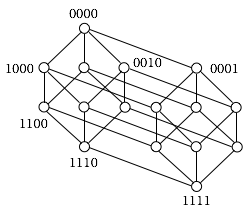
\includegraphics[scale=0.6]{FiguresGraph/Isomorphism1}
       \caption{A representation of $\q_4$ with partial coding of the vertices.}
  \label{fig:isomorphism1}
\end{center}
\end{figure}

\begin{figure}[hbt]
\begin{center}
       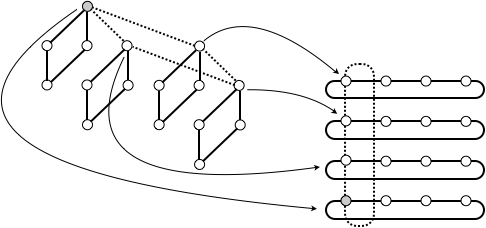
\includegraphics[scale=0.5]{FiguresGraph/Isomorphism2}
       \caption{Transformation of $\q_4$ to a $4 \times 4$ torus.
       The bold edges correspond to the horizontal cycles and the dashed edges correspond to vertical cycles.}
  \label{fig:isomorphism2}
\end{center}
\end{figure}

A graphical proof is depicted in Fig.~\ref{fig:isomorphism1}  and ~\ref{fig:isomorphism2} and 
We relegate the formal proof of this result to a Exercise
{\Denis add a ref here?}, supplying as a
hint the coding scheme (or, bijection) depicted in
Fig.~\ref{fig:toruslabel}.
\begin{figure}[hbt]
\begin{center}
       \includegraphics[scale=0.6]{FiguresGraph/toruslabel}
\caption{Sketching the coding scheme that yields an isomorphism
  between the order-$4$ hypercube $\q_4$ and the $4 \times                          
4$ torus $\widetilde{\m}_{4,4}$.}
  \label{fig:toruslabel}
\end{center}
\end{figure}


\subsubsection{The de Bruijn network $\d_n$}
\label{sec:deBruijn-network}
\index{de Bruijn network}
\index{de Bruijn graph}

While the family of hypercube networks has few competitors in the
world of parallel and distributed computing, in terms of performance
and ease of designing algorithms, it does have one major shortcoming
regarding its realization in hardware.  The basic problem is that the
order-$n$ hypercube has large node-degrees, specifically logarithmic
in the size of the network.  This feature makes the hypercubes actual
performance much lower than its theoretical performance.
Specifically, the size of the hypercube grows exponentially with the
common degrees of the network's nodes---this is the ``inverse'' way
of talking about logarithmic node-degrees---while the space in which
we (and our computers) live grows only cubically with linear
distance.  The resulting disparity means that the wires in a large
computing platforms connected by an hypercube must inevitably be very long---in contrast to the unit-size
of idealized network-edges.  Consequently, electrical signals within a
large hypercube must travel long distances, which means that the
physical computer is much slower than its idealized version.  (One
finds a more technical discussion of this phenomenon in
\cite{Ullman84}.)

The preceding shortcoming of hypercubes led researchers to seek a
family of networks whose node-degrees stay constant even as one
deploys successively larger instances of the network.  A candidate
such network was discovered within the domain of coding theorists (as,
coincidentally, was the hypercube).  

In the mid-20-century, Dutch mathematician Nicolaas Govert de Bruijn
\index{de Bruijn, Nicolaas Govert} discovered a way to generate
compact sequences that contain all possible strings of a prespecified
length.  Focussing on {\em binary} strings---although de Bruijn's
strategy works for any finite alphabet---de Bruijn could generate a
string of length $2^n +n-1$ that contains every length-$n$ binary
string as a substring.  Quite appropriately, such a string is called a
{\it de Bruijn sequence}. \index{de Bruijn sequence} It is not obvious
that de Bruijn sequences exist for every $n$, but we now plant the
seeds of a proof that they do.  We begin by illustrating two sample
sequences in (\ref{eqn:deBruijn-seq}).
\begin{equation}
\label{eqn:deBruijn-seq}
\begin{array}{|l||c|c|}
\hline
n & \mbox{\sc Length-$n$ binary strings}
    & \mbox{\sc Order-$n$ de Bruijn sequence} \\
\hline
\hline
1 &
00, \ 01, \ 10, \ 11  & 00110 \\
\hline
2 &
\begin{array}{l}
000, \ 001, \ 010, \ 011, \\
100, \ 101, \ 110, \ 111 
\end{array}
  & 0001110100 \\
\hline
\end{array}
\end{equation}
The table in (\ref{eqn:deBruijn-seq}) spawns several interesting
questions:
\begin{itemize}
\item
Do de Bruijn sequences exist for every $n$?
\item
If so, 
  \begin{itemize}
  \item
How does one compute them?
  \item
Can one always find a de Bruijn sequence of length $2^n +n-1$?
  \item
Can one find de Bruijn sequences of length $< 2^n +n-1$?
  \end{itemize}
 \ignore{
 {\Arny (SOME GOOD EXERCISES HERE)} 
 }
\end{itemize}
The answers to all of these questions---and the connection of de
Bruijn sequences to the current chapter---reside in the family of
directed graphs called {\it de Bruijn graphs} (or, {\it networks}).
\index{de Bruijn graph} \index{de Bruijn network} (The term used
varies by intended application---mainly, coding theory and [the
  interconnection networks of] parallel computer architectures.  We
use the names interchangeably.)

\begin{figure}[hbt]
\begin{center}
       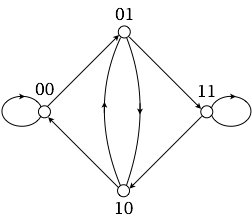
\includegraphics[scale=0.5]{FiguresGraph/dB2by2}
       \caption{The $4$-node, order-$2$ de Bruijn network.}
  \label{fig:dB2by2}
\end{center}
\end{figure}

\begin{figure}[hbt]
\begin{center}
       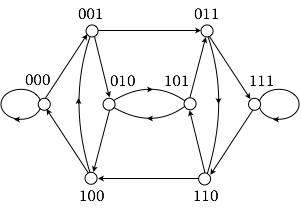
\includegraphics[scale=0.6]{FiguresGraph/dB2by3}
       \caption{The $8$-node, order-$3$ de Bruijn network.}
  \label{fig:dB2by3}
\end{center}
\end{figure}

For every integer $n \in \N^+$, the {\it order-$n$ de Bruijn network}
is the {\em directed} graph $\d_n$ whose nodes comprise the set of
length-$n$ binary strings.\footnote{While {\em binary} de Bruijn
  networks are the most frequently encountered ones, one can also find
  de Bruijn networks whose nodes comprise all length-$n$ strings over
  larger finite alphabets.  Such extended families also find
  applications in coding theory.}  The sets $\n_{\fd_2}$ and
$\n_{\fd_3}$ appear in (\ref{eqn:deBruijn-seq}).


$\d_n$ is a regular directed graph; its nodes all have in-degree $2$
and outdegree-$2$.  Each node of $\d_n$ is a binary string of
length $n \geq 1$; hence it can be written in the form $\beta x$,
where $\beta \in \{0, \ 1\}$ is a {\it bit} (short for {\it binary
  digit}) and $x$ is a length-$(n-1)$ binary string.

The $2^{n+1}$ arcs of $\d_n$ come in pairs specified as follows.  For
each $\beta \in \{0,1\}$ and for each length-$(n-1)$ binary string
$x$, $\d_n$ has the two arcs
\[ (\beta x \rightarrow x0) \ \ \ \mbox{ and } \ \ \ 
(\beta x \rightarrow x1)
\]
We enumerate $\a_{\fd_3}$ in (\ref{eqn:deBruijn-arcs}).
\begin{equation}
\label{eqn:deBruijn-arcs}
{\small
\begin{array}{|ccccc|}
\hline
\mbox{\sc Source node} & & \mbox{\sc Target node} & & \mbox{\sc Target node} \\
\hline \hline
{\displaystyle
\left.
\begin{array}{c}
000 \\
001 \\
010 \\
011 \\
100 \\
101 \\
110 \\
111
\end{array}
\right\}
} &
\mbox{\sc goes to} 
  &
{\displaystyle
\left\{
\begin{array}{c}
000 \\
010 \\
100 \\
110 \\
001 \\
011 \\
101 \\
111
\end{array}
\right.
}
  &
\mbox{\sc and to}
  &
{\displaystyle
\left\{
\begin{array}{c}
001 \\
011 \\
101 \\
111 \\
000 \\
010 \\
100 \\
110
\end{array} 
\right.
}
 \\
\hline
\end{array}
}
\end{equation}

For each $n \in \N^+$, $\d_n$ has diameter $n$.  To see why this is
true, note that following any one of $\d_n$'s arcs, say from node $x$
to node $y$, consists of ``rewriting'' the length-$n$ string $x$ as
the length-$n$ string $y$.  The diameter bound therefore follows by
showing that, for any two string-nodes of $\d_n$, say node $u$ and
node $v$, one can rewrite string $u$ as string $v$ by traversing a
sequence of arcs---i.e., a directed path---of length at most $n$.
Observe, for instance, that the path in $\d_3$ described schematically
as follows
\[ 000 \ \rightarrow \ 001 \ \rightarrow \ 011 \ \rightarrow \ 111 \]
leads node $000$ to node $111$, by rewriting string $000$ as string
$111$.  The diameter bound is now an immediate consequence of the
following result.  The result builds upon a notion that we have not
yet encountered but will study in some detail in
Section~\ref{sec:Hamiltonian-cycle}
\index{graphs!Hamiltonian cycle} \index{Hamiltonian cycle}.

A {\it Hamiltonian cycle} in an $n$-node graph $\g$ is a length-$n$
cycle that contains every node of $\g$ precisely once.  A {\it
  directed Hamiltonian cycle} in an $n$-node digraph $\h$ is a
length-$n$ directed cycle that contains every node of $\h$ precisely
once.

\begin{prop}
\label{thm:deBruijn-Hamiltonian}
For all $n \in \N^+$, $\d_n$ contains a {\em directed Hamiltonian
  cycle}, 
\index{directed Hamiltonian cycle in a digraph}
i.e., a length-$2^n$ directed cycle of the form
\begin{equation}
\label{eq:deBruijn-cycle}
 x \ \rightarrow \ y_1 \ \rightarrow \ y_2 \ \rightarrow \cdots
\ \rightarrow \ y_{2^n-1} \ \rightarrow \ x
\end{equation}
that contains every node of $\d_n$ precisely once; i.e.:
\begin{itemize}
\item
$\{x, \ y_1, \ y_2, \ldots, \ y_{2^n-1}\} \ = \ \n_{\fd_n}$.
\item
All of the ``$y$-nodes'' that appear in cycle
(\ref{eq:deBruijn-cycle}) differ from $x$ and from each other.
\end{itemize}
\end{prop}

The simplest proof of this result has two steps, each of which
introduces a topic we have not yet developed.

{\Denis Add a word here about hamiltonian and Eulerian and refer to the appendix...}

\ignore{

\noindent {\bf (1)}
%
For any directed graph $\g$, the {\it line digraph} \index{line graph}
\index{line digraph} of $\g$, denoted $\Lambda(\g)$, is the following
directed graph.
\begin{itemize}
\item
The nodes of $\Lambda(\g)$ are the arcs of $\g$:
\[ \n_{{\Lambda}({\cal G})} \ = \ \a_{\fg} \]
\item
For each pair of arcs of $\g$ of the form
\[ \big[a_{x,y} = (x \ \rightarrow \ y) \big] \ \ \ \mbox{ and } \ \ \ 
\big[a_{y,z} = (y \ \rightarrow \ z) \big]
\]
i.e, arcs such that the endpoint of the first arc is the source of the
second arc, $\Lambda(\g)$ contains an arc $(a_{x,y} \ \rightarrow
\ a_{y,z})$.
\end{itemize}
The relevance of this topic to this section is that the line graph of
every de Bruijn network $\d_n$ is the ``next bigger'' de Bruijn
network, $\d_{n+1}$.  Let us verify this claim.

\begin{prop}
\label{thm:deBruin-linegraph}
For all $n \in \N^+$,
$\d_{n+1}$ is the line digraph of $\d_n$: $\d_{n+1} \ = \ \Lambda(\d_n)$.
\end{prop}

\begin{proof}
Each node of $\Lambda(\d_n)$ is an arc of $\d_n$, hence has the form
\[ (\beta x \ \rightarrow \ x \gamma) \]
for $x$ a length-$(n-1)$ binary string and $\beta, \gamma \in
\{0,1\}$.  Let us associate node $\beta x \gamma$ of $\d_{n+1}$ with
this node of $\Lambda(\d_n)$.

\smallskip

Note first that each arc of $\d_{n+1}$ has the form
\[ (\delta y \varepsilon \ \rightarrow \ y \varepsilon \varphi), \]
where $y$ is a length-$(n-2)$ binary string and $\delta, \varepsilon,
\varphi \in \{0,1\}$.  By our association of nodes of $\d_{n+1}$ with
arcs of $\d_n$, this arc of $\d_{n+1}$ does, indeed, correspond to two
successive arcs of $\d_n$.   The first of these successive arcs
{\em enters} node $y \varepsilon$ of $\d_n$; the second {\em leaves}
that node.

Note next that, given any two successive arcs of $\d_n$, say
\[
(\rho \sigma z \ \rightarrow \ \sigma z \tau) \ \ \ \mbox { and } \ \ \
(\sigma z \tau \ \rightarrow \  z \tau \xi)
\]
where $z$ is a length-$(n-2)$ binary string and $\rho, \sigma, \tau,
\xi \in \{0,1\}$, there is, indeed, an arc of $\d_{n+1}$ of the form
\[ (\rho \sigma z \tau \ \rightarrow \ \sigma z \tau \xi) \]
This means that the digraph $\d_{n+1}$ is identical to the digraph
$\Lambda(\d_n)$, modulo a renaming of nodes and arcs.\footnote{Technically,
  we are asserting that the digraphs ${\cal D}_{n+1}$ and ${\Lambda}({\cal D}_n)$ 
  are {\it isomorphic} to one another.  The topic of
  graph isomorphism is beyond the scope of this text, but our informal
  description provides all the details one would need to formalize the
  described isomorphism.}

The described correspondence between the nodes and arcs of $\d_{n+1}$
and $\Lambda(\d_n)$ completes the proof.  \qed
\end{proof}

\begin{figure}[hbt]
\begin{center}
       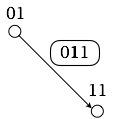
\includegraphics[scale=0.6]{FiguresGraph/dBlabelEdge}
\caption{Illustrating how to label each arc of a de Bruijn network by
  concatenating the labels of the nodes incident to the arc and
  compacting the common intermediate bits.  In the depicted example,
  the node-labels $01$ and $11$ combine to yield the arc-label $011$.}
  \label{fig:dBlabelEdge}
\end{center}
\end{figure}

\medskip

\noindent {\bf (2)}
{\it Eulerian cycles (or tours)}. \index{Eulerian cycle}
\index{Eulerian tour} A {\it directed Eulerian cycle} in a digraph
$\g$ is a directed cycle that contains each arc of $\g$ precisely
once.  We will see, later in this chapter, a truly elementary
argument, based on node-degrees, which proves that every de Bruijn
digraph has a directed Eulerian cycle.  This demonstration will
combine with Proposition~\ref{thm:deBruin-linegraph} to complete the
proof of Proposition~\ref{thm:deBruijn-Hamiltonian}.  \qed
%\end{proof}
}

\bigskip

Stepping back from the structural specifics of $\d_n$, we now see that
de Bruijn networks provide us with a {\em
  bounded-degree---specifically, a degree-$2$} family of networks each
of whose constituent graphs has {\em logarithmic diameter}!  In this
regard, at least, de Bruijn networks have exactly the same
cost-performance as hypercubes---i.e., $2^n$-node graphs with diameter
$n$---with bounded degrees.  Even more dramatic, it has been shown
that sophisticated algorithmic techniques can achieve roughly
equivalent computational efficiency, on a broad range of significant
computational problems, using de Bruijn networks as using like-sized
hypercubes \cite{AnnexsteinBR90, BermondP89, Ullman84}.



%%%%%%%%%%%%%%%%%%%%%%%%%%%%%%%%%%%

\section{Graph Coloring and Chromatic number}
\label{sec:graph-color}
\index{graphs!node-coloring}

This section introduces the notion of {\it graph coloring}, and its
associated notion of the {\it chromatic number}
\index{graphs!chromatic number} of a graph.

A {\it node-coloring} \index{graphs!node-coloring} of a graph $\g$ is
an assignment of labels to $\g$'s nodes, in such a way that all of a
node $v$'s neighbors get a different label than $v$.  Traditionally,
the labels are called {\it colors}, for that term's evocative power.
The {\it chromatic number} \index{graphs!chromatic number} of a graph
$\g$ is the smallest number of colors that can be used in a legal
node-coloring of $\g$.  In traditional parlance, the assertions

``$\g$ has chromatic number $c$'' \ \ \ \ \ and \ \ \ \ \
``$\g$ is {\it $c$-colorable}''
\index{graphs!$c$-colorable}

\noindent
are considered to be synonymous.

{\Denis I added the following remark, do you agree?}
This notion is an important characteristic of a graph.
It is like an intermediate concept between the degree (local)
and diameter (global), which are easy to compute. 
The chromatic number is not easy to compute.
\bigskip

\noindent \fbox{
\begin{minipage}{0.95\textwidth}
The notion of graph coloring can be used to computational advantage to
model a broad variety of situations.  An extremely important, and
illustrative, use of graph coloring is to model {\it distributed}
computing.  In this setting, the nodes of a computation-graph $\g$
represent {\it agents}, such as, e.g., processing elements in a
computer; and $g$'s edges represent {\it communication links} that
enable each node $u$ to check its neighbors' states before any action
and to inform its neighbors of state-changes occasioned by an action
of $u$.  
{\Denis actually, coloring is useful in any situation to express incompatibility between items}
The prohibition against ``monochrome'' edges---i.e., edges
both of whose incident nodes have the same color---guarantees that
node $u$ and all of its like-colored nodes can act at the same instant
with no fear of missing an important input to those actions.  Indeed,
one often encounters programs for distributed computing that look
something like

1. All {\em red} nodes perform an action

2. All {\em green} nodes perform an action

3. All {\em blue} nodes perform an action

\hspace*{1in} $\vdots$
\end{minipage}
}

\subsection{Graphs with Small Chromatic Numbers}
\label{sec:Graphs-small-Chromatic-No} 

Most of the ``named'' graphs in
Section~\ref{sec:graphs-important-families} have very small chromatic
numbers.  This is no accident: These graphs were invented (or, at
least, placed in the spotlight) because of their importance to the
topic of parallel and distributed computing---and we suggested only a
few paragraphs ago how to use graph node-colors to orchestrate some
such computations.  Accordingly, we devote this section to studying
graphs with very small chromatic numbers.

\subsubsection{Graphs with chromatic number $2$}
\label{sec:2-color-graphs}

We begin to garner intuition about graph coloring by exposing a large
set of graphs with chromatic number $2$.  In fact, we can completely
characterize these graphs structurally.

A graph $\g$ is {\it leveled} \index{graphs!leveled} if there exists
an assignment of {\it level numbers} $\{ 1, 2, \ldots, \lambda\}$ to the
nodes of $\g$ in such a way that every neighbor of a level-$\ell$ node
$u$ resides either on level $\ell +1$ or on level $\ell -1$.

\begin{prop}
\label{thm:leveled=2-color}
A graph $\g$ has chromatic number $2$ if, and only if, it is leveled.
\end{prop}

\begin{proof}
Say first that $\g$ is a leveled graph.  Then labeling each node of
$\g$ with the (odd-even) parity of its level provides a valid
$2$-coloring of $\g$.

Say next that $\g$ is $2$-colorable.  Pick any node $v$ of $\g$ and
assign it to be the unique node on level $1$.  Let all neighbors of
$v$ be assigned to level $2$.  Continuing iteratively, say that the
largest level-number that we have employed---i.e., assigned nodes
to---is $\ell$.  Then we now assign to level $\ell +1$ all neighbors
of level-$\ell$ nodes which have not yet been assigned to a level of
$\g$.  Because $\g$ is $2$-colorable, each of the levels we have
specified is monochromatic, so that each edge of $\g$ connects a node
of one color with a node of the other color.  \qed
\end{proof}

We can now show that the following named graphs are $2$-colorable.

\begin{corol}
\label{thm:list-2-colorables}
The following graphs are leveled, hence have chromatic number $2$.

{\bf (a)}
any tree (which includes any path-graph $\p_n$)
{\Denis check here is path graph has well been defined before... Or include a reference}

{\bf (b)}
any cycle-graph $\cc_n$ that has an even number $n$ of nodes

{\bf (c)}
any mesh-graph $\m_{m,n}$

{\bf (d)}
any torus-graph $\widetilde{\m}_{m,n}$ that has an even number of
diagonals, i.e., even $m+n$

{\bf (e)}
any hypercube $\q_n$
\end{corol}

\begin{proof}
We provide a detailed sketch for each of the five graph families in
turn.

\noindent {\bf (a)}
We follow the procedure from the second half of the proof of
Proposition~\ref{thm:leveled=2-color} to expose a level structure in
any tree $\t$, as follows.  Pick any node $v$ of $\t$ and make it the
unique node on level $1$.  Let all neighbors of $v$ be assigned to
level $2$.  Continuing iteratively, say that the largest level-number
that we have employed is $\ell$.  Then we now assign to level $\ell
+1$ all neighbors of level-$\ell$ nodes which have not yet been
assigned to a level of $\t$.

Of course this process can be simplified when $\t$ is a path-graph
$\p$, by choosing one of $\p$'s end-nodes as node $v$.  We thereby
have precisely one node on each level, whereas the general procedure
can have levels with $2$ nodes.  A lesson here is that {\em a graph
  may admit many distinct level structures}.

\medskip

\noindent {\bf (b)}
When we apply the procedure of part (a) to an even-length cycle
$\cc_{2n}$, we produce a level structure in which levels $1$ and $n+1$
have one node apiece, while all other levels have two nodes apiece.

\medskip

\noindent {\bf (c)}
The edge-structure of mesh-graphs ensures that the labeling of each
node $\langle i,j \rangle$ of $\m_{m,n}$ with the odd-even parity of
the number $i+j$ is a $2$-coloring of $\m_{m,n}$.

\medskip

\noindent {\bf (d)}
The labeling in part (d) provides a $2$-coloring of any torus-graph
$\widetilde{\m}_{m,n}$ with even $m+n$.

\medskip

\noindent {\bf (e)}
Each edge of a hypercube $\q_n$ connects a node $v = \beta_1 \beta_2
\cdots \beta_n$, where each $\beta_i \in \{0,1\}$, to a node $v' =
\beta'_1 \beta'_2 \cdots \beta'_n$ where precisely one $\beta_j$
differs from $\beta'_j$.  Therefore, the following aggregation of
nodes of $\q_n$ into sets $S_0, S_1, \ldots, S_n$ provides a valid
leveling of $\q_n$.

Assign node $v = \beta_1 \beta_2 \cdots \beta_n$ to set $S_k$
precisely if $k$ of the bits $\beta_i$ equal $1$.
\qed
\end{proof}

The reader can show that no odd-length cycle $\cc_{2n+1}$ with $n \geq
1$ is $2$-colorable.  In like fashion, no graph $\g$ that {\em
  contains} an odd-length cycle can be $2$-colored.  This is the
problem that plagues the torus $\widetilde{\m}_{m,n}$ when $m+n$ is
odd.
\ignore{  {\Arny Put the odd cycle and torus as Exercises}}

The existence of odd-length cycles prevents {\em every} de Bruijn
network $\d_n$ from being $2$-colorable.  As small examples, one
observes the $3$-cycle
\[ 00 \ \rightarrow \ 01 \ \rightarrow \ 10  \rightarrow \ 00 \]
in $\d_2$ in Fig.~\ref{fig:dB2by2} and the $3$-cycle
\[ 001 \ \rightarrow \ 010 \ \rightarrow \ 100 \ \rightarrow \ 001 \]
in $\d_3$ in Fig.~\ref{fig:dB2by3}.  In fact, these small odd-length
cycles are only the proverbial tip of the iceberg for de Bruijn
networks.  The following result asserts that de Bruijn networks are
{\it directed-pancyclic}, \index{graphs!pancyclic} 
\index{de Bruijn network!pancyclicity} \index{de Bruijn graph!pancyclicity}
meaning that they contain (even directed!)~cycles of {\em all}
possible lengths, both odd and even.  The proof of this result is
outside the scope of this text, but it should be accessible to the
motivated reader.

\begin{prop}{\cite{Yoeli62}}
For all $n$, the order-$n$ de Bruijn
network $\d_n$ is directed-pancylic, i.e., it
contains directed cycles of all possible lengths $1, 2, \ldots, 2^n$.
\end{prop}

\subsubsection{Planar and Outerplanar Graphs}
\label{sec:planar+outerplanar-color}
\index{planar graphs}
\index{outerplanar graphs}
\index{graphs!planar}
\index{graphs!outerplanar}

In this section, we focus on two graph families that are defined in
terms of the way they can be drawn (on a two-dimensional medium, such
as a piece of paper).
\bigskip

\noindent \fbox{
\begin{minipage}{0.95\textwidth}
The reader should not view this attention to how a graph can be drawn
as just an abstract game.  The process of designing and implementing
circuits within the constraints of {\it VLSI}, \index{VLSI} {\it Very
  Large Scale Integrated Circuit} technology,
\index{Very Large Scale Integrated Circuit technology}
\index{VLSI:Very Large Scale
Integrated Circuit technology} are very similar to drawing a circuit
on a two-dimensional medium.  We refer the reader to the revolutionary
1979 text \cite{Mead-Conway} for an introduction to this fascinating
technology, which requires technical literacy but little specialized
knowledge.
\end{minipage}
}
\bigskip

\noindent
A graph is {\it planar} \index{graphs!planar} \index{planar graphs}
precisely if it can be drawn {\em without any crossing edges}.  A
graph $\g$ is {\it outerplanar} \index{graphs!outerplanar}
\index{outerplanar graphs} precisely if it can drawn by {\em placing
  its nodes along a circle in such a way that its edges can be drawn
  as noncrossing chords of the circle}.  The latter condition is
equivalent to demanding that $\g$'s edges can be drawn within the
circle without any crossings.

We urge the reader to garner intuition about the graphs in these
families by experimenting with drawing some specific, rather complex
graphs.
\begin{itemize}
\item
The first set of graphs to draw are cliques, as defined in
Section~\ref{sec:clique}.  The cliques $\k_3$, $\k_4$, and
$\k_5$ will help expose the nature of the planar and outerplanar
graphs, because:
  \begin{itemize}
  \item
$\k_3$ is outerplanar; 
  \item
$\k_4$ is planar but not outerplanar;
  \item
$\k_5$ is not planar.
  \end{itemize}

\item
The ``bipartite'' cousins of the cliques will also yield valuable
insights.  For postive integers $m$ and $n$, the $m \times n$
bipartite clique $\k_{m,n}$ \index{bipartite clique} is the graph
whose node-set comprises the ordered pairs of integers:
\[  \n_{\fk_{m,n}} \ = \
\{ \langle i,j \rangle \ \ | \ \ 1 \leq i \leq m; \ \ 1 \leq j \leq n\}
\]
and whose edges connect each node $\langle i,j \rangle$ to every node
$\langle i,k \rangle$ with $1 \leq k \leq n$ and to every node
$\langle h,j \rangle$ with $1 \leq h \leq m$.

The second set of graphs to draw are the bipartite cliques $\k_{1,3}$,
$\k_{2,3}$, and $\k_{3,3}$.  These graphs will also help expose the
nature of the planar and outerplanar graphs, because:
  \begin{itemize}
  \item
$\k_{1,3}$ is outerplanar; 
  \item
$\k_{2,3}$ is planar but not outerplanar;
  \item
$\k_{3,3}$ is not planar.
  \end{itemize}
\end{itemize}

We selected the preceding cliques and bipartite cliques to ``play
with'' very carefully.  Using arguments that go beyond the scope of
this text, one can prove the following {\em characterization via
  exclusion} result, which characterizes each of our graph families by
identifying {\it forbidden subgraphs}.  \index{forbidden subgraphs}
\index{forbidden subgraphs!characterization of planar graphs}
\index{forbidden subgraphs!characterization of outerplanar graphs} The
notion of {\it graph homeomorphism} plays a fundamental role in
\index{graphs!homeomorphism} the characterization.  This is a
dauntingly named technical term that is easily understood informally.
A {\it homeomorph} \index{graphs!homeomorph} of a graph $\g$ is
obtained by adding (degree-$2$) nodes along one or more edges of $\g$.
The characterization of planar graphs by exclusion resides in a
celebrated theorem by the Polish mathematician and logician Kazimierz
Kuratowski; \index{Kuratowski, Kazimierz} the analogous result for
outerplanar graphs was derived by the French mathematician Gary
Chartrand \index{Chartrand, Gary} and the American mathematician Frank
Harary. \index{Harary, Frank}

\begin{theorem}
\label{thm:planar+outerplanar-exclusion}
{\bf (a)} {\rm \cite{ChartrandB67}}
A graph is outerplanar if, and only if, it does not have a subgraph
that is homeomorphic to either $\k_4$ or $\k_{2,3}$.

{\bf (b)} {\rm \cite{Kuratowski30}}
A graph is planar if, and only if, it does not have a subgraph
that is homeomorphic to either $\k_5$ or $\k_{3,3}$.
\end{theorem}


\paragraph{\small\sf A. Outerplanar graphs}

We look first at the smaller of this section's graph families, namely,
the {\it outerplanar graphs}. \index{outerplanar graphs}
\index{graphs!outerplanar} (We shall remark in the following subsection B why these
graphs are called {\em outer}-planar.)

We begin our discussion of outerplanar graphs with some basic facts
about the family.

\begin{prop}
Every tree is outerplanar.
\end{prop}

We leave to the reader the challenge of proving this property. 
As an help, Fig.~\ref{fig:treeoutplanar} shows the way to distribute the nodes along a circle for the graph of Fig.~\ref{fig:tree}.

\begin{figure}[hbt]
\begin{center}
       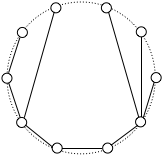
\includegraphics[scale=0.5]{FiguresGraph/TreeOutplanar}
       \caption{Outerplanar representation of the tree of Fig~\ref{fig:tree}.}
  \label{fig:treeoutplanar}
\end{center}
\end{figure}

\ignore{
We leave to the reader the challenge of drawing a tree in a way that
exposes its outerplanarity.  
{\Arny Another exercise}
}

\begin{prop}
\label{thm:basic-outerplanar-stuff}
Let $\g$ be an outerplanar graph.  Then:

\begin{tabular}{ll}
{\bf (a)} &
$\g$ is planar. \\
\ignore{{\bf (b)} &
$\g$ is a subgraph of a Hamiltonian graph. 
{\Denis I removed the second item since Hamiltonian has been shifted after this section.}\\}
{\bf (b)} &
Every subgraph of $\g$ is outerplanar. \\
{\bf (c)} &
At least one of $\g$'s nodes has degree $\leq 2$.
\end{tabular}
\end{prop}

\begin{proof}
{\bf (a)} $\g$'s planarity can be inferred from the ability to draw
$\g$'s edges as noncrossing chords of the circle.

\medskip
\ignore{
\noindent {\bf (b)} $\g$'s ``sub-Hamiltonianicity'' can be inferred
from the ability to draw $\g$ with its nodes along a circle.

\medskip}

\noindent {\bf (b)} We can produce an outerplanarity-witnessing
drawing of any subgraph of $\g$ by erasing some nodes and/or some
edges from our outerplanarity-witnessing drawing of $\g$.

\medskip

\noindent {\bf (c)} One verifies easily that this result holds for all
outerplanar graphs having $3$ or fewer nodes.  Focus, therefore, on an
arbitrary outerplanar graph $\g$ that has more than $3$ nodes.  Since
adding more edges to a graph cannot decrease the degree of any node,
we lose no generality by focusing on a graph $\g$ that is {\em maximal}
outerplanar, \index{maximal outerplanar graph} in the sense that
adding any new edge to $\g$ would destroy its outerplanarity.

Because $\g$ has more than $3$ nodes, and because all of its nodes lie
on a circle (in the drawing that witnesses its outerplanarity), there
must be pairs of nodes of $\g$ that are not adjacent along the circle.
Let $u$ and $v$ be nonadjacent nodes such that the distance between
$u$ and $v$ (measured in term of number of edges that must be traversed to reach one
from the other) is minimal among pairs of nodes nonadjacent nodes.  We
consider two cases.
\begin{itemize}
\item
If the distance between $u$ and $v$ were $2$, then the unique node
that lies between $u$ and $v$ along the circle would have degree $2$.
\item
If, on the other hand, the distance between $u$ and $v$ {\em exceeded}
$2$, then there would be at least {\em two} nodes that lie between $u$
and $v$ in either direction around the circle.  But in this case,
there would be two nonadjacent nodes that were closer to one another
than $u$ and $v$---which contradicts our choice of $u$ and $v$ as a
pair of closest nonadjacent nodes.
\end{itemize}
We conclude that $\g$ must have a node of degree $\leq 2$, completing
the proof.
\qed
\end{proof}

\bigskip

Our primary concern in this section is, of course, on graph coloring.
We return to this topic now.  The $3$-node cycle $\cc_3$ witnesses the
fact that not every outerplanar graph is $2$-colorable; $3$ colors is
the best that we can hope for.  We now show that this hope can be
realized.  The inductive proof of the following result can easily be
turned into an efficient node-coloring algorithm for outerplanar
graphs.

\begin{prop}[The $3$-Color Theorem for Outerplanar Graphs]
\label{thm:OP-3-colorability}
Every outerplanar graph is $3$-colorable.
\end{prop}

\begin{proof}
We proceed by induction on the number of nodes in the outerplanar
graph to be colored.

The base cases of the result are provided by small outerplanar
graphs---say those having $3$ nodes or fewer.

We assume, for induction, that every outerplanar graph having fewer
than $n$ nodes is $3$-colorable.

Let us now focus on an arbitrary $n$-node outerplanar graph $\g$.  By
Proposition~\ref{thm:basic-outerplanar-stuff}(d), $\g$ has a node $v$
of degree $\leq 2$.  Let us remove node $v$ from $\g$, along with the
edge(s) that connect $v$ to the rest of $\g$; call the resulting graph
$\g'$.  Now, $\g'$ is clearly outerplanar, once we ``stitch'' together
the circle we ``damaged'' by removing $v$, and $\g'$ has fewer than
$n$ nodes.  By induction, therefore, $\g$ is $3$-colorable.  But now
we can reattach node $v$ to $\g'$ by replacing the edges that attach
$v$ to $\g$.  Moreover, we can now color $v$ using whichever of the
$3$ colors on $\g$ that is {\em not} used for $v$'s neighbors in $\g$.
We have, thus, specified a $3$-coloring of $\g$, which extends the
induction and completes the proof.  \qed
\end{proof}

\ignore{**************
Two remarks about Proposition~\ref{thm:OP-3-colorability}:
\begin{enumerate}
\item
Our proof of the proposition can easily be transformed into an
algorithm that $3$ colors any $n$-node outerplanar graph in a
number of inductive stages that is a low-degree polynomial in $n$.
\item
The color-bound of the proposition can, of course, not be improved, as
witnessed by odd-length cycle-graphs.
\end{enumerate}
*************}


\paragraph{\small\sf B. Planar graphs}

The larger of this section's two graph families comprises {\it planar
  graphs} \index{planar graphs} \index{graphs!planar} i.e., graphs
that can be drawn (on a two-dimensional medium, such as a piece of
paper) with no crossing edges.  The original focus on planar graphs
stemmed from viewing them as abstractions of geographical maps.

The $4$-node clique $\k_4$ witnesses the fact that not every planar
graph is $3$-colorable.  To wit, because every pair of nodes of every
clique are neighbors of each other, it follows that:

\smallskip

{\em For all $n$, the $n$-node clique $\k_n$ can be colored with $n$
  colors but no fewer.}.

\smallskip

\noindent
A century-plus attempt to prove that $4$ colors suffice for planar
graphs culminated in one of the most fascinating dramas in modern
mathematics, as American mathematicians Kenneth Appel 
\index{Appel, Kenneth}
and Wolfgang Haken, \index{Haken, Wolfgang}---with the help of their
families and of their computer!---announced their two-article-long
proof in 1974 of their renowned {\it $4$-Color Theorem for Planar
  Graphs}.  \index{The $4$-Color Theorem for Planar Graphs}
\index{coloring planar graphs!the $4$-Color Theorem}

\begin{theorem}[The $4$-Color Theorem for Planar Graphs~\cite{AppelH77a,AppelH77b}]
\label{thm:Four-ColorTheorem}
Every planar graph is $4$-colorable.
\end{theorem}

The proof of Theorem~\ref{thm:Four-ColorTheorem} is beyond the scope
of any introductory text, but the backstory of the proof is truly
fascinating---and it supplies ample motivation for the proofs of the
$6$-color and $5$-color analogues of the Theorem.  Beginning with a
failed attempt, in 1875, to prove that every planar map can be colored
with four colors with no abutting countries getting the same color,
the so-called {\it $4$-Color Problem}
\index{The $4$-Color Problem for planar graphs} 
held the world of discrete mathematics in thrall for roughly a century
before But the drama surrounding the $4$-Color Problem persisted,
because of the Appel-Haken proof's reliance, in a fundamental way, on
a computer program that checked more than a thousand essential---but
clerical---assertions (about forbidden subgraphs).  It took the
mathematics community years before this proof, with its massive
complexity and unprecedented employment of ``collaboration'' by
computer, was generally accepted.  In addition to the primary
references \cite{AppelH77a,AppelH77b} that accompany our statement of
the Theorem, we recommend to the interested reader the articles
\cite{AppelH77c,AppelH89} that summarize and, at a rather
sophisticated level, popularize this marvelous mathematical tale.

We turn now to the $6$-color and $5$-color analogues of the $4$-color
Theorem.  The weaker, $6$-color, version of the Theorem can be proved
in much the same way as its outerplanar-graph cousin,
Proposition~\ref{thm:OP-3-colorability}.  The proof of the stronger,
$5$-color, version of the Theorem already requires us to break the
world into multiple cases---but only a single-digit number of cases,
in contrast to the four-digit case list one encounters with the proof
of Theorem~\ref{thm:Four-ColorTheorem} \cite{AppelH77a,AppelH77b}.

\bigskip

{\it The $6$-Color Theorem for Planar Graphs.}
The first step in showing that every planar graph can be colored using
$6$ colors resides in the following analogue for planar graphs of
Proposition~\ref{thm:basic-outerplanar-stuff}(d), which asserts that
every outerplanar graph has a node of degree $2$.

\begin{lemma}
\label{thm:PlanarGraph-degree5}
Every planar graph has a node of degree $\leq 5$.
\end{lemma}

\begin{proof} {\em (Lemma~\ref{thm:PlanarGraph-degree5})}
Let us focus on a planar drawing of a (perforce) planar graph $\g$,
which has $n$ nodes, $e$ edges, and $f$ {\it faces}.  A {\it face}
\index{graphs!planar!face in a drawing}
\index{planar graph!face in a drawing} 
in a drawing of $\g$ is a polygon whose sides are edges of
$\g$, whose points are nodes of $\g$, and whose interiors are empty,
in that no edge of $\g$ crosses through the interior.
\bigskip

\noindent \fbox{
\begin{minipage}{0.95\textwidth}
Now that we know about faces, we can finally describe the origin of
the term {\it outerplanar}.  A graph $\g$ is outerplanar if it can be
drawn with all of its nodes around a single ``outer'' face in such a
way that all of its edges are drawn in a noncrossing manner within the
``outer'' face.  In fact, we usually draw $\g$ so that the ``outer''
face is literally outside the ``outer'' face.
\end{minipage}
}
\bigskip

The following auxiliary result derives a celebrated ``formula'' of
Euler.  \index{Euler, Leonhard} \index{Euler's Formula}

\begin{prop} [Euler's Formula for Planar Graphs]
\label{thm:Euler-Formula}
Given the indicated drawing of $\g$, we have
\begin{equation}
\label{eqn:Eulers-formula}
n \ - \ e \ + \ f \ \ = \ \ 2
\end{equation}
\end{prop}

\medskip

We defer proving Proposition~\ref{thm:Euler-Formula} so that we can
proceed with our ongoing proof of Lemma~\ref{thm:PlanarGraph-degree5}.
\ignore{{\Denis Attention here: the ref is not written correctly after the compilation}}
We devote Subsection C to two quite different proofs of Euler's
celebrated formula.

\medskip

As we approach the next step of the proof, we simplify the setting by
assuming henceforth that $\g$ is connected and that it is {\em
  maximal}, \index{graphs!planar!maximal} in the sense that one cannot
add any new edge to the drawing without crossing an existing edge.
This step only strengthen's the Lemma's conclusion by apparently
making it more difficult to find a small-degree node.

With this assumption in place, we now adapt a pedagological tool from
\cite{Berge73}, in order to make the following counting argument
easier to follow.  We construct a {\em directed bipartite} graph {\bf
  G} which exposes certain features of $\g$'s structure.  On one side
of {\bf G} are the $f$ faces of $\g$; on the other side are $\g$'s $e$
edges.  {\bf G} contains an arc from each face of $\g$ to
each edge of $\g$ that forms a ``side'' of the polygonal
drawing of the face.  Because $\g$ is a maximal planar graph, we have:
\begin{itemize}
\item
Each face of $\g$ is a $3$-cycle, hence involves three nodes.
\item
Each edge of $\g$ touches two faces.
\item
Each edge of $\g$ touches two nodes.
\end{itemize}

Let us now put these facts together, and assume, for contradiction,
that every node of $\g$ had degree $\geq 6$.  We would then find that
\[
\left[ f \ \ \leq \ \ \frac{2}{3} e \right] \ \ \ \ \mbox{ and } \ \ \ \
\Big[ e \ \ \geq \ \ 3n \Big]
\]
Incorporating these two bounds into Euler's Formula
(\ref{eqn:Eulers-formula}), we arrive at the following contradiction.
\[ 2 \ \ = \ \ n \ - \ e \  + \ f
\ \ \leq \ \ \frac{1}{3} e \ - \ e \ + \ \frac{2}{3} e \ \ = \ \ 0
\]
This contradiction proves that every planar graph must have a node of
degree $\leq 5$.
 \qed-Lemma~\ref{thm:PlanarGraph-degree5}
\end{proof}

\medskip

We finally have the tools to color planar graphs using $6$ colors.
\index{The $6$-Color Theorem for Planar Graphs}
\index{coloring planar graphs!the $6$-Color Theorem}

\begin{prop}[The $6$-Color Theorem for Planar Graphs]
\label{thm:P-6-colorability}
Every planar graph is $6$-colorable.
\end{prop}

\begin{proof}
The $2$-Color Theorem for Outerplanar Graphs
(Proposition~\ref{thm:OP-3-colorability}) and this result follows via
almost-identical inductions on the number of nodes in the graph $\g$
that is being colored.  Both arguments:
\begin{enumerate}
\item
remark that the coloring goal can be met for small graphs

For outerplanar graphs, ``small'' means ``$3$ or fewer nodes''.  For
planar graphs, it means ``$4$ or fewer nodes''.

\item
remove from $\g$ a node $v$ of smallest degree $d_v$, together with
all its incident edges

For outerplanar graphs, we guarantee that $d_v \leq 2$
(Proposition~\ref{thm:basic-outerplanar-stuff}(d)).  For planar
graphs, we guarantee that $d_v \leq 5$
(Lemma~\ref{thm:PlanarGraph-degree5}).

\item
inductively color the nodes of the graph $\g'$ left after the removal
of $v$

For outerplanar graphs, we color $\g'$ with $\leq 3$ colors
(Proposition~\ref{thm:OP-3-colorability}).  For planar
graphs, we use an inductive assumption that $\g'$ can be colored with
$\leq 6$ colors. 

\item
reattach $v$ via its $d_v$ edges and then color $v$.

Note that the coloring guarantee in both
results---Proposition~\ref{thm:OP-3-colorability} for outerplanar
graphs and the current result for planar graphs---allows us to use
$d_v +1$ colors to color $\g$.  Because $v$ has degree $d_v$, it is a
neighbor of no more than $d_v$ nodes of $\g'$, so our access to $d_v
+1$ colors guarantees that we can successfully color $v$.
\end{enumerate}
The proofs of the $3$-colorability of outerplanar graphs and the
$6$-colorability of planar graphs thus differ only in the value of
$d_v$.  \qed
\end{proof}

\bigskip

{\it The $5$-Color Theorem for Planar Graphs.}
\index{The $5$-Color Theorem for Planar Graphs}
\index{coloring planar graphs!the $5$-Color Theorem}
We now prove that every planar graph can be colored using $5$ colors.
\bigskip

\noindent \fbox{
\begin{minipage}{0.95\textwidth}
The case analysis in the following proof is a bit more complex than in
most of the results in the text, but a methodical reading should make
the proof quite accessible.  Moreover, {\em roadmap} of the case
analysis is a valuable lesson in how mathematics is really done!  For
instance, the motivated reader will be able to recast the totally
positive proof we present into the form of a proof by contradiction.
The positive version should be more to the taste of a computationally
oriented reader---but both proofs are equally correct.
\end{minipage}
}
\bigskip

\begin{prop}[The $5$-Color Theorem for Planar Graphs \cite{Heawood90}]
\label{thm:5colors}
Every planar graph is $5$-colorable.
\end{prop}

\ignore{************************
The proof again (I mean like for 6 colors) is by recurrence but we add
here a contradiction argument:
Similarly, we focus on a node with degree 5 (at some points, we will
have to justify this)
This node (call it x) has 5 neighbors
The problem is when they are colored by the 5 colors, otherwise it is
colored by a missing one.
Let now label these 5 nodes from 1 to 5.
Consider the nodes 1 and 3, colored by two different colors and the
sub-graph composed of nodes with colors 1 and 3
If these two nodes are in disjoint connected components, (case 1), it is
easy to color x by reverting the colors 1 and 3 in one component
(see figure)
Thus, the problem is when there exists an alternate path (in term of
colors) between node 1 and node 3
in this case (case 2), consider nodes 2 and 4, using a similar process
as in case 1, if there are two connected components
we are done (x can be colored by reverting the colors along the path
in one component), otherwise, there is an alternate path
between 2 and 4.
However, since the graph is planar, then, both alternate paths will
intersect, which is impossible
************************}


The proof is rather technical and thus, it is shifted to the Appendix~\ref{Appendix:5colors}.
It combines a sophisticated analysis of the structure of the
planar graph we wish to color with an induction that can be converted
into an efficient algorithm actually achieving the $5$-coloring.

\ignore{
\begin{proof}
For brevity, let us henceforth discuss only {\em valid} colorings,
i.e., colorings of a graph's nodes in which neighboring nodes get
different colors.

\smallskip

\noindent {\em Base of our induction.}
Because the $5$-clique $\k_5$ is obviously $5$-colorable, so also must
be all graphs having $\leq 5$ nodes.  Therefore, we know that any
non-$5$-colorable graph would have $\geq 6$ nodes.

\smallskip

\noindent {\em Inductive hypothesis.}
Assume, for induction, that every planar graph having $\leq n$ nodes
is $5$-colorable.

\smallskip

\noindent {\em Inductive extension.}
If the proposition were false, then there would exist a planar graph
$\g$ having $n+1$ nodes which is not $5$-colorable.  By
Lemma~\ref{thm:PlanarGraph-degree5}, $\g$ would have a node $v$ of
degree $\leq 5$.  The remainder of the proof focuses on the graph
$\g$, its minimal-degree node $v$, and on $v$'s $(d_v \leq 5)$
neighbors in $\g$.

Now, if there were a coloring of $\g$'s nodes in which $\leq 4$ colors
were used to color $v$'s neighbors, then the following analogue of the
coloring strategy of Proposition~\ref{thm:P-6-colorability} would
produce a $5$-coloring of $\g$.
\begin{enumerate}
\item
Remove node $v$ and its incident edges from $\g$, thereby producing
the $n$-node planar graph $\g'$.
\item
Produce a $5$-coloring of $\g'$ that uses only $4$ colors for the
nodes that are neighbors of $v$ in $\g$.
\item
($a$) Reattach node $v$ and its edges to $\g'$, thereby reconstituting
  $\g$.  ($b$) Color $v$ with whichever of the $5$ available colors is
  not used to color $v$'s neighbors.
\end{enumerate}

In order to proceed in pursuit of a contradiction, we must understand
what structural features of $\g$ make it impossible to use only $4$
colors on $v$'s neighbors when $5$-coloring $\g$.  There are three
important situations to recognize.
\begin{description}
\item[{\sf Case 1}.]
Node $v$ has degree $\leq 4$.

\smallskip

By definition, $\leq 4$ colors are used to color $v$'s neighbors in
this case.
\end{description}
Note that, in all remaining cases, node $v$ has precisely $5$
neighbors---or else, we would have invoked Case 1 to color $\g$ with
$5$ colors.
\begin{description}
\item[{\sf Case 2}.]
For some $5$-coloring of $\g$, $\geq 2$ neighbors of $v$ get the same
color.

\smallskip

Because $v$ has exactly $5$ neighbors, in this case, only $4$ colors
are used to color these neighbors.
\end{description}
In all remaining cases, the $5$ neighbors of $v$ receive distinct
colors.
\begin{description}
\item[{\sf Case 3}.]
For some $5$-coloring of $\g$, some two neighbors of $v$, call them
$v_1$ and $v_2$, reside in distinct components of $\g$ once $v$ and
its incident edges are removed from $\g$.

\smallskip

As before, let $\g'$ be the (in this case, disconnected) graph that
results when $v$ and its incident edges are removed from $\g$.  For $i
= 1,2$ Let $\g_i$ be the component of $\g'$ that contains node $v_i$.

Say that, under the $5$-coloring of $\g$ that we are focusing on,
$v_1$ is colored {\it red} and $v_2$ is colored {\it green}.

Let us recolor the nodes of $\g_1$ so that node $v_1$ is now colored
{\it green}.  (One needs only switch the colors {\it red} and {\it
  green} in the existing coloring of $\g_1$.)  It is always possible
to do this in a way that does not affect the valid coloring of $\g_2$
because $\g_1$ and $\g_2$ are mutually disjoint.

Once we have thus-recolored $\g_1$, we have a $5$-coloring of $\g$ for
which Case 2 holds.  (In fact, we can color node $v$ {\em red} when we
reattach it to $\g'$.)
\end{description}

\noindent
We now see that Cases 1--3 cannot prevent us from $5$-coloring $\g$, so
we are left with the following minimally constrained situation.
\begin{description}
\item[{\sf Case 4}.]
\begin{itemize}
\item
Every minimum-degree node of $\g$ has $5$ neighbors.

For the minimum-degree node $v$, let us call these neighbors $v_1$,
$v_2$, $v_3$, $v_4$, $v_5$, in clockwise order within the planar
drawing.
\item
In every $5$-coloring of $\g$, the neighbors of every minimum-degree
node receive distinct colors.

For node $v$, let us say that neighbor $v_i$ receives color $c_i$.
\end{itemize}
The leftmost graph in FIGURE 1 
{Denis Put right ref here}
depicts the portion of $\g$ comprising
node $v$ and its neighbors.  In the figure, we use integer $i$ to
denote, ambiguously, node $v_i$ and its assigned color $c_i$.  The
question mark ``?'' that ``colors'' node $v$ indicates that we do not
yet know what color to assign to $v$.  The other two graphs in the
figure depict schematically how we have dealt with Case 3 above.
\begin{itemize}
\item
All neighbors of node $v$ remain in the same component of $\g$ when
$v$ and its incident edges are removed.
\end{itemize}
\end{description}
To analyze Case 4, we focus on nodes $v_1$ and $v_3$ in FIGURE 1.
{Denis Put right ref here}
Importantly, these nodes have received distinct colors ($c_1$ and $c_3
\neq c_1$, respectively), and these nodes are not adjacent to one
another as one makes a clockwise sweep around node $v$.

Now take $\g$ and focus only on the nodes that are colored $c_1$ or
$c_3$ (as are $v_1$ and $v_3$, respectively) and on the nodes that are
colored $c_2$ or $c_4$ (as are $v_2$ and $v_4$, respectively).  One
sees from Figure 2 that:
\begin{itemize}
\item
$\g$ can, {\em but need not}, contain a path whose nodes alternate
  colors $c_1$ and $c_3$---call this a ``$c_1$-$c_3$ path'' between
  nodes $v_1$ and $v_3$.
\item
$\g$ can, {\em but need not}, contain a path whose nodes alternate
  colors $c_2$ and $c_4$---call this a ``$c_2$-$c_4$ path'' between
  nodes $v_2$ and $v_4$.
\item
$\g$ {\em cannot} contain both of the paths just described, i.e., a
  $c_1$-$c_3$ path between $v_1$ and $v_3$ {\em and} a $c_2$-$c_4$ path
  between $v_2$ and $v_4$.

{\em These two paths, if they existed, would cross one another---which
  is forbidden because $\g$ is a {\em planar} graph.}  See Figure 2.
\end{itemize}
It follows that {\em either} $\g$ does not contain a $c_1$-$c_3$ path
between $v_1$ and $v_3$ {\em or} $\g$ does not contain a $c_2$-$c_4$
path between $v_2$ and $v_4$.  Say, with no loss of generality, that
the former path does not exist.  Then we can switch colors $c_1$ and
$c_3$ beginning with node $v_1$ and obtain a coloring of $\g$ in which
$v_1$ and $v_3$ both receive the color $c_3$.  We can then proceed as
in Case 2 to get a $5$-coloring of $\g$.

This four-case analysis shows that we can always produce a
$5$-coloring of $\g$, which completes the proof.  \qed
\end{proof}
}

We finish this topic with an overview of the intellectual
cost-benefit tradeoff we have observed:
\begin{itemize}
\item
A straightforward recursive coloring strategy suffices if one is
willing to settle for a six-color palette when coloring planar graphs
(Proposition~\ref{thm:P-6-colorability}).
\item
A four-case analysis, in which one case comprises multipl subcases, is
needed in order to eliminate one of the colors from the palette, to
achieve a five-color palette (Proposition~\ref{thm:5colors}).
\item
An analysis involving close to $2000$ cases is needed in order to
achieve the provable optimal, a four-color palette
(Theorem~\ref{thm:Four-ColorTheorem}).
\end{itemize}

\paragraph{\small\sf C. Two validations of Euler's Formula}
\index{Euler's Formula}

We develop two quite different proofs of
Proposition~\ref{thm:Euler-Formula}.

\medskip

\index{Euler's Formula!validation by structural induction}
\noindent {\bf Validatinging Euler's Formula by structural induction}.  We
validate (\ref{eqn:Eulers-formula}) by growing a planar graph $\g$
edge by edge.  We proceed by induction.

\smallskip

\noindent {\it Base case}.
The Formula clearly holds for the smallest planar graphs, including
the smallest interesting one, $\cc_3$, which has $n = e = 3$ and $f =2$
(the inner and outer faces of the ``triangle'').

\smallskip

\noindent {\it Extension}.
We grow the current version of $\g$ by adding a new edge.  Two cases
arise.
\begin{itemize}
\item
{\em The new edge connects existing nodes.}  In this case, this
augmentation of $\g$ increases the number of edges ($e$) and the
number of faces ($f$) by $1$ each, while keeping the number of nodes
($n$) unchanged.  Euler's Formula (\ref{eqn:Eulers-formula}) thus
continues to hold.

\item
{\em The new edge adds a new node, which is appended to some
  preexisting node.}  In this case, this augmentation of $\g$
increases the number of edges ($e$) and the number of nodes ($n$) by
$1$ each, while keeping the number of faces ($f$) unchanged.  Euler's
formula (\ref{eqn:Eulers-formula}) thus continues to hold.
\end{itemize}
This augmentation extends the induction, hence validates the Formula.
\qed

\bigskip

%{\Denis Here is a nice alternative proof for the Euler proposition}

\index{Euler's Formula!validation by deconstruction}
\noindent {\bf Validating Euler's Formula by deconstruction}.  Let us be
given a planar graph $\g$ that has $n$ nodes, $e$ edges, and $f$
faces.  We validate (\ref{eqn:Eulers-formula}) by deconstructing $\g$
and showing that each step in the process preserves as {\it invariant}
the expression $\phi(n,e,f) = n-e+f$.  \index{invariants}

\bigskip

\noindent \fbox{
\begin{minipage}{0.95\textwidth}
The concept of \textit{invariance} is an extremely important
conceptual tool when crafting proofs.  The underlying idea is to find
an expression $\phi(\cdot)$ whose value is preserved as a process
proceeds, step by step.  Rather than try to explain the concept in
abstraction, we recommend that the reader follow this proof of Euler's
Formula with an eye to keeping track of the invariant expression
$\phi(n,e,f)$ whose arguments are obtained from the subject planar
graph $\g$.
\end{minipage}
}
\bigskip

\noindent
We analyze the following two-phase process performed in sequence.
\begin{description}
\item[{\bf Phase 1}.]
Iterate the following process of removing edges from $\g$ until one
edge-removal reduces $\g$ to a graph with a single face.  This
termination condition is equivalent to stopping when the remaining
graph is a tree.  One can verify that the tree one ends up with is
{\em connected}.
\bigskip

{\bf The action}.
If the graph remaining at some step contains an edge that is shared by
two distinct faces, then remove any such edge.

Fig.~\ref{fig:planarStep1} illustrates the action of Step 1 for a
(residual) graph with $n=8$ nodes, $e=11$ edges, and $f=5$ faces.
\begin{figure}[hbt]
\begin{center}
   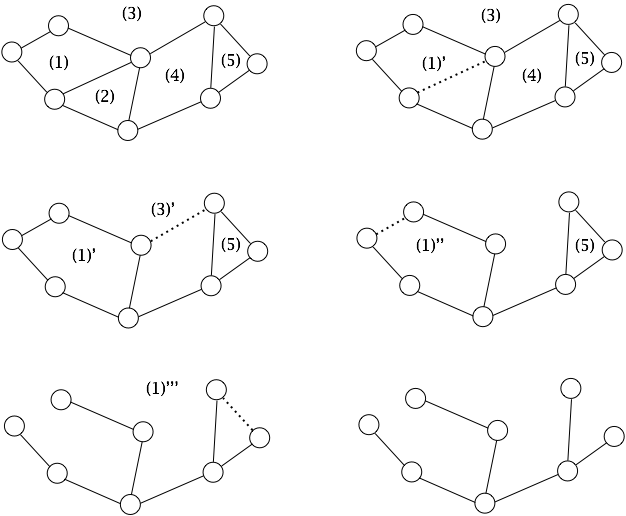
\includegraphics[scale=0.4]{FiguresGraph/planarStep1}
\caption{Illustrating Phase 1: From top left to bottom right, each
  transformation preserves the invariant $\phi(n,e,f)$.  The first
  transformation removes the edge shared by faces (1) and (2),
  creating a new, merged, face (1)'.}
  \label{fig:planarStep1}
\end{center}
\end{figure}

\bigskip

{\bf The analysis}.
\begin{itemize}
\item
The graph remaining after an edge-removal is still planar---edges are
removed but never added---so we can continue the process.
\item
The process preserves the value of function $\phi$.  To wit, $n$ is
unchanged, while $e$ and $f$ are each reduced by $1$: $\phi(n,e,f) =
\phi(n,e-1,f-1)$.
\end{itemize}

\item[{\bf Phase 2}.]
Iterate the following process of removing nodes from the tree produced
by Step 1, until only one node remains.
\bigskip

{\bf The action}.
Remove any leaf of the current tree, together with its incident edge.

Fig.~\ref{fig:planarStep2} illustrates the action of Step 2
for a tree  with $n=8$ nodes---hence, $e=7$ edges and $f=1$ face.
\begin{figure}[hbt]
\begin{center}
   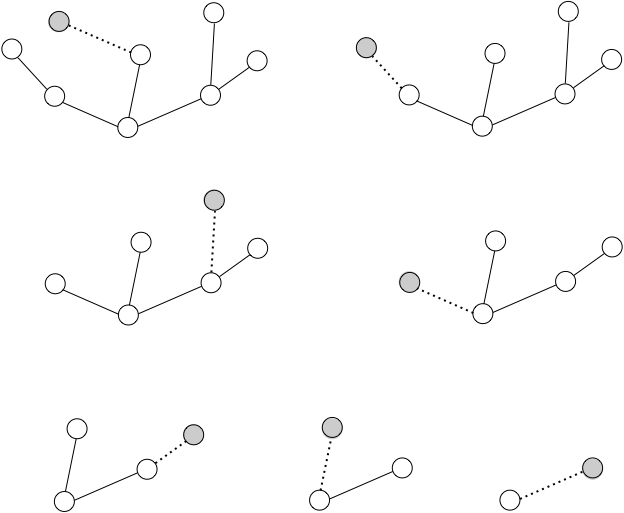
\includegraphics[scale=0.4]{FiguresGraph/planarStep2}
   \caption{Illustrating Phase 2: We remove a sequence of leaves, each
     with its incident edge, until we reach a single node.  Again,
     $\phi$ remains invariant after each leaf-removal.}
  \label{fig:planarStep2}
\end{center}
\end{figure}

\bigskip

{\bf The analysis}.
The value of function $\phi$ remains unchanged by each leaf-removal.
To wit, $f$ is unchanged (it remains at $1$), while $n$ and $e$ are
each reduced by $1$: $\phi(n,e,f) = \phi(n-1,e-1,f)$
\end{description}

\noindent {\bf The cumulative analysis}.
\begin{itemize}
\item
Our process executes a number of steps exactly equal to the number of
edges of the graph $\g$ that we began with.  To wit, the edge-removal
Step removes $e-n$ edges, while the leaf-removal Step removes $n$
nodes.
\item
At the end of the process, $e=0$ and $n=f=1$, so that the residual
value of $\phi$ is $2$.  Because each action prescribed by the process
preserved the value of $\phi$, we know that $\phi$ has the value $2$
before each edge-removal and leaf-removal.
\end{itemize}
We conclude that, at the
start of the process,  $\phi(n,e,f)$ had the value $2$.  In other
words, $n-e+f = 2$.  This concludes the proof.  \qed

\bigskip

\noindent \fbox{
\begin{minipage}{0.95\textwidth}

**ADD REFERENCES HERE

We presented several parameters for characterizing a graph.
The degree of the vertices (which is a local characteristic) 
and the diameter (which is a global characteristic).
Both parameters are easy to determine (done in polynomial time).
The chromatic number is an intermediate concept which provide a global information from local rules.
It is hard to compute for any graph. 

\cite{GareyJ79}
\cite{Karp72}

It is an {\sf NP}-complete problem to decide, given any fixed $k \geq
3$, whether a given graph $\g$ is $k$-colorable.

A simple argument shows that it is {\sf NP}-hard to find smallest
number of colors that provide a valid node-coloring of $\g$.

But one can exhibit ``greedy'' algorithms that give good results.
\end{minipage}
}


\section{Path and Cycle Discovery Problems in Graphs}
\label{sec:path-cycle-problems}

Just as various genres of {\it spanning trees} are used to
``summarize'' aspects of the connectivity structure of a connected
graph $\g$, various genres of {\it paths} and {\it cycles} in $\g$ are
often useful to ``summarize'' aspects of $\g$'s traversal structure.
This section is devoted to a range of problems related to determining
the existence in a graph $\g$ of a path or a cycle that {\em
  completely} ``summarizes'' $\g$'s traversal structure, either by
containing each node of $\g$ precisely once or by containing each edge
of $\g$ precisely once.  We shall generally focus in this section only
on {\em undirected} paths and cycles in {\em undirected}, {\em
  unweighted} graphs.  Extrapolating the notions we discuss to their
directed analogues in directed and/or weighted graphs, will be
accomplished via carefully crafted exercises.  In a similarly, but
simpler, vein, we shall generally discuss only prolems concerning {\em
  cycles}, leaving to the reader the analogous notions that concern
paths.  We begin by delimiting the two main classes of cycle-discovery
problems that we study in this section.

\smallskip

{\it Eulerian cycles (or, tours)}.  A cycle in a graph $\g$ that
traverses each of $\g$'s edges precisely once is called an {\it
  Eulerian cycle},\index{graphs!Eulerian cycle} \index{Eulerian cycle}
(or, often, an {\it Eulerian circuit}).  \index{graphs!Eulerian
  circuit} \index{Eulerian circuit} The edge-exhausting
cycles/circiuts/tours referred to by these several names were
introduced as a topic of study in 1736 by the Swiss mathematician
\index{Euler, Leonhard} Leonhard Euler, whose name we have already
encountered multiple times.  Euler allegedly discovered the topic
while contemplating how to design a tour of the town of K\"{o}nigsberg
that would cross each of the town's bridges precisely once.  The quest
for Eulerian cycles in graphs is, thus, one of the oldest problems in
the fields now called {\it Operations Research} and {\it graph
  theory}.  (An edge-exhausting {\em path} in $\g$ is referred to in
the obvious analogous way.)  When one views an Eulerian cycle as a
``map'' for traversing a graph---as did Euler when contemplating this
problem---one often calls the cycle an {\it Eulerian tour}.
\index{graphs!Eulerian tour} \index{Eulerian tour} Traditionally, a
graph that admits an Eulerian cycle is said to be {\it
  Eulerian}. \index{graphs!Eulerian} \index{Eulerian graph}

\medskip

Dually: A cycle in a graph $\g$ that encounters each of $\g$'s nodes
precisely once is called a {\it Hamiltonian cycle},
\index{graphs!Hamiltonian cycle} \index{Hamiltonian cycle} (or, often,
a {\it Hamiltonian circuit}). \index{graphs!Hamiltonian circuit}
\index{Hamiltonian circuit} This cycle-discovery problem is named in
honor of the British mathematician Sir William Rowan Hamilton,
\index{Hamilton, William Rowan} who is credited with inventing the
concept in the mid-19th century.  
{\Denis even if the problem was introduced some time before in its whole genericity by 
Thomas Penyngton Kirkman} (A node-exhausting {\em path} in
$\g$ is referred to in the obvious analogous way.)  When one views a
Hamiltonian cycle as a ``map'' for traversing a graph, one often calls
the cycle a {\it Hamiltonian tour}.  \index{graphs!Hamiltonian tour}
\index{Hamiltonian tour} Traditionally, a graph that admits a
Hamiltonian cycle is said to be {\it
  Hamiltonian}. \index{graphs!Hamiltonian} \index{Hamiltonian graph}

\medskip

Despite the conceptual duality between the edge-encountering goal that
underlies Eulerian paths and cycles, on the one hand, and the
node-encountering goal that underlies Hamiltonian paths and cycles,
these two graph-traversing goals differ in virtually every significant
respect.  It is rather easy to characterize the family of graphs that
admit Eulerian tours and to find such a tour if it exists
(Section~\ref{sec:EulerianCycle}); in contrast, there is no known
characterization of the family of graphs that admit Hamiltonian tours,
and the computational problem of efficiently determining whether a
graph admits such a tour is one of the major classical problems in the
field of computational complexity  (Section~\ref{sec:Hamiltonian-cycle}).

%%%%%%%%%%%%%%%%%%%%%%%%%%%%%%%%%%%%%%%%%%%%%%%%%%%%

\subsection{Eulerian Cycles and Paths}
\label{sec:EulerianCycle}

The main results in this section characterize the families of directed
and undirected graphs that admit an {\it Eulerian cycle} or an {\it
  Eulerian path}.  The proofs of these characterizations are
constructive: they consist of algorithms that efficiently find such a
cycle or such a path when one exists.  We focus on graphs that are
connected: the algorithms we present can actually be adapted to find
an {\it Eulerian cycle} or an {\it Eulerian path} in each connected
component of a general graph.  As we embark on our adventure, we note
that the problem of finding an Eulerian cycle in a graph $\g$ is
equivalent to the problem of drawing $\g$ without ever lifting one's
pencil. \index{graphs!drawing without lifting pencil}

%\subsubsection{Characterizing Eulerian graphs, and finding Eulerian tours}
%\label{sec:eulerian-cycle-path}

There is a simple and elegant characterization of graphs that admit
Eulerian cycles and paths, which is accompanied by a simple and
efficent algorithm for testing a given graph for finding such a tour
in a graph that admits one.  We encapsulate four versions of the
desired result in the following statement.

\begin{prop}[Eulerian Cycles]
\label{thm:eulerian-cycle}
{\bf (a)}
An undirected graph $\g$ admits an Eulerian cycle if, and only if,
$\g$ is connected and every node of $\g$ has even degree.

{\bf (b)}
A directed graph $\h$ admits a directed Eulerian cycle if, and only if,
$\h$ is connected and, for every node $v$ of $\g$,
$\mbox{\sc indegree}(v) \ = \ \mbox{\sc outdegree}(v)$.
\end{prop}

\begin{proof}
The {\em necessity} of the conditions in both parts {\bf (a)} and {\bf
  (b)} is established by the two following observations.
\begin{itemize}
\item
By definition, a graph that is not connected does not admit any \textit{eulerian} cycle.
\item
Each cycle that a graph admits accounts for two edges per node,
because the cycle must ``enter'' the node by one edge and ``exit'' the
node by a different edge.
\end{itemize}

\smallskip

\noindent
We turn now to the verification of the {\em sufficiency} of the
Proposition's conditions.  Our argument resides in the following
``streamlined'' version of an induction---this is closer to the form
of an induction that one would encounter in practice, rather than in a
textbook.

The base case of the induction resides in proving the sufficiency of
the Proposition's conditions for ``small'' graphs.  
\bigskip

\noindent \fbox{
\begin{minipage}{0.95\textwidth}
While we largely
leave this step to the reader, we do want to discuss the definition of
``small''.  Until we understand how to deal with arbitrary $n$-node
graphs, we will not know how the general step of our induction reduces
the graph size $n$ at each step.  Because of this, it is a good
practice to ``play'' with several small graph sizes initially.
Hopefully, in addition to giving our inductive argument a robust base
case, such ``playing'' will give us valuable intuition for the general
case of the induction.
\end{minipage}
}


\begin{itemize}
\item
Focusing on {\em undirected} graphs: We note that $2$-node graphs
cannot have even node-degrees---and, indeed, as promised by the
Proposition, they cannot be Eulerian.  One can exhaustively enumerate
$3$-node and $4$-node graphs and verify that the Proposition correctly
separates the Eulerian ones from the non-Eulerian ones.
\item
Focusing on {\em directed} graphs: We note that $2$-node graphs can be
Eulerian---as witnessed by the $2$-node digraph each of whose nodes
hosts a single arc that points to the other node.  Once again, one can
perform an exhaustive enumeration of $3$-node and $4$-node graphs
and verify that the Proposition correctly separates the Eulerian ones
from the non-Eulerian ones.
\end{itemize}

We now develop a complete proof of the {\em sufficiency} of the
conditions in part {\bf (a)} of the Proposition, for general $n$-node
undirected graphs.  Throughout the discussion, we intersperse hints
regarding the sufficiency of the conditions in part {\bf (b)} of the
Proposition.

Let us consider a connected multi-node undirected graph $\g$ all of
whose nodes have nonzero even degree.
{\Denis  should'nt multi-node be defined? What do you mean here?}

\begin{description}
\item[{\bf Step 1}]
Initialize the {\it progress parameter} $k$ to $0$.  This parameter
will help orchestrate our discovery of the Eulerian cycle within $\g$.
{\Denis no need to step 1}

\item[{\bf Step 2}]
Choose an arbitrary node of $\g$ some of whose incident edges have not
yet been traversed.  Call this node $v_k$, and let us henceforth refer
to $v_k$ as a {\em special} node.  Follow a walk along edges of $\g$
beginning at special node $v_k$.  
{\Denis we should change $v_k$ to $v$ if we change the way to write the proof...}
The rules of this walk are:
\begin{itemize}
\item
Every step of the walk will traverse an edge of $\g$ that {\em has not
  yet been traversed} during any walk.
\item
The walk terminates when it encounters a node of $\g$ {\em all of
  whose edges have already been traversed}.
\end{itemize}
The facts that 

\hspace*{.25in}\begin{tabular}{ll}
(1) & each node of $\g$ has even degree; \\
(2) & the walk begins at node $v_k$ (which crosses one of $v_k$'s edges); \\
(3) & no edge of $\g$ is traversed more than once
\end{tabular}

\noindent
mean that the last node encountered in this walk is $v_k$.  In other
words: {\em This walk begins and ends with node $v_k$.}

Note that node $v_k$ will occur in this walk multiple
times---specifically with multiplicity $\frac{1}{2} \mbox{\sc
  degree}(v_k)$.
  
{\Denis Denis I would suggest here to simply a bit, in fact both  steps 1 and 2 aims simply at determining a non-empty cycle in the graph...}

We have completed the walk in $\g$ that begins and ends at node $v_k$.

{\Denis I suggest to skip step 3... I think it is enough -- and more easy-- to build
the whole eulerian cycle from any cycle. Do I miss something?}

\ignore{\smallskip
\item[{\bf Step 3}]
Say that we have completed the walk in $\g$ that begins at node $v_k$.

{\bf If} every edge of $\g$ has been traversed by the end of the
current walk, then we {\it go to {\bf Step 4}} and invoke procedure
{\bf Build Eulerian Cycle}, which stitches our series of walks into an
Eulerian cycle in $\g$.

\smallskip

{\bf Else}, there is a node of $\g$, call it $v_{k+1}$, one of whose
incident edges has not yet been traversed.  Note that we are here
increasing the value of our progress parameter from $k$ to $k+1$.  We
now {\it repeat {\bf Step 2}} with the updated progress parameter,
$k+1$.
}

\item[{\bf Step 4}]
\ignore{We have reached this step because our sequence of walks that begin and
end at special nodes has terminated with all of $\g$'s edges having
been traversed.}

The previous step determined a cycle in graph $\g$,.
Once it is removed, it remains several connected components,
denoted by $\mathcal{C}_1$, $\mathcal{C}_2$, $\ldots$ $\mathcal{C}_c$.
This cycle intersects the strong components at nodes $v_1$, $v_2$ until $v_c$. 
We are now ready to exhibit an Eulerian cycle in $\g$ by going piece after piece along the cycle 
starting from $v_k$.
{\Denis change it to $v$}

\end{description}

\ignore{The resulting procedure
{\bf Build Eulerian Cycle} proceeds as follows.

For each special node $v_k$, during the walk that begins and ends at
$v_k$, we encounter other special nodes, call them $v_{k,1}$,
$v_{k,2}$, \ldots, $v_{k,{m_k}}$, in the order of their being
encountered along the walk.  We then define the following recursive
procedure.
{\Denis it is not really recursive since each procedure is only called once...}

\medskip

\begin{tabular}{|ll|}
\multicolumn{2}{l}{{\bf Procedure Build Eulerian Cycle}($v_k$)} \\
\hline
{\bf Phase $1$} &
Follow the walk that begins at $v_k$ until it encounters $v_{k,1}$ \\
  &
Execute {\bf Build Eulerian Cycle}($v_{k,1}$) \\
\hline
{\bf Phase $2$} &
Continue the walk that begins at $v_k$ until it encounters $v_{k,2}$ \\
  &
Execute {\bf Build Eulerian Cycle}($v_{k,2}$) \\
\hline
  &
$\begin{array}{c}
\bullet \\
\bullet \\
\bullet
\end{array}
$ \\
\hline
{\bf Phase $m_k$} &
Continue the walk that begins at $v_k$ until it encounters $v_{k,m_k}$ \\
   &
Execute {\bf Build Eulerian Cycle}($v_{k,m_k}$) \\
\hline
{\bf Phase $m_k +1$} &
Complete the walk that begins at $v_k$. \\
\hline
\end{tabular}
\end{description}

\medskip

\noindent
The process invocation

Execute {\bf Build Eulerian Cycle}($v_0$)

\noindent
produces the Eulerian cycle in $\g$.
}

\bigskip

When dealing with a {\em directed} graph, we proceed exactly as
with undirected graphs, with one critical difference: for each node
$v$ we always enter $v$ along one of its {\em in-arcs}, and
we always exit $v$ along one of its {\em out-arcs}.  As in the
undirected case, each arc is traversed precisely once during
the described process.  \qed
\end{proof}


\ignore{**************
We offer two proofs of this result: the first merely establishes the
existence of the cycle; the second actually computes the cycle.  Both
proofs invoke the following elementary facts.
\bigskip
\noindent {\bf Claim 1.}
if all the degrees are even (and not null) then there exists a cycle.\bigskip
\noindent {\bf Claim 2.}
A tour is an union of disjoint cycles.\bigskip
\noindent {\bf Claim 3.}
If we remove a cycle in a tour then the degrees remain even.\bigskip
\begin{proof}
{\bf A proof of existence.}


The necessary condition of the proposition is straightforward. 
Let us focus on the sufficient condition.
\bigskip

\noindent {\bf Proof 1 (existence).}

By contradiction, let us assume that all the vertices of a connected graph are even and there is no tour that contains all the edges.
Let consider a tour with a maximum number of edges. 
If we remove its edges, it remains some edges and from Claim~3 they are even.
Then, from Claim~1, there exists a cycle within these remaining edges (say $\Gamma$). 
The contradiction comes from Claim~2 since the union of the maximal tour plus the cycle $\Gamma$ 
is another tour which contains more edges than the initial one.
\bigskip

\noindent This proof can be adapted in a constructive way and thus, leads to an algorithm. It is as follows:

\noindent {\bf Proof 2 (constructive).}
By induction on the number of edges. 

\begin{itemize}
\item The basis case is simple to verify for $m=2$ (where two vertices linked by two edges correspond to the cycle of minimal length). 
\item
Let consider a connected graph with $m+1$ edges where all its vertices have an even degree.
Let assume that the property holds for connected graphs of even vertices with $k$ edges ($k \leq m$), which means there exist Eulerian tours in these sub-graphs. 

From Claim~1, there exists a cycle (let denote it by $\Gamma$ described by its successive vertices) and consider the sub-graph of $G$ 
without the edges of $\Gamma$: $G'=(V-{\Gamma},E')$. 
By induction hypothesis, there exists an Eulerian cycle $\mathcal{C}_i$ in each connected component of $G'$ 
(from Claim 3).
The Eulerian tour of $G$ is obtained by the concatenation of pieces of $\Gamma$ and the Eulerian cycles in the successive $\mathcal{C}_i$.

\end{itemize}
*****************}

The simplicity of the preceding characterisation degrades a trifle when
one seeks Eulerian {\em paths} rather than {\em cycles}.

\begin{prop}[Eulerian Paths]
\label{thm:eulerian-path}
{\bf (a)}
An undirected graph $\g$ admits an Eulerian path if, and only if,
$\g$ is connected and at most two nodes of $\g$ have odd degree.

{\bf (b)}
A directed graph $\h$ admits an Eulerian path if, and only if: $\h$ is
connected; either $\h$ admits an Eulerian cycle, or $\h$ contains one
node $u$ such that

\hspace*{.5in}$\mbox{\sc indegree}(u) \ = \ \mbox{\sc outdegree}(u) +1$

\noindent
and one node $v$ such that

\hspace*{.5in}$\mbox{\sc indegree}(v) \ = \ \mbox{\sc outdegree}(v) -1$.
\end{prop}

The proof of the path-oriented Proposition~\ref{thm:eulerian-path} has
the same overall structure as the cycle-oriented
Proposition~\ref{thm:eulerian-cycle}, with one major difference.
Whereas a cycle has neither beginning nor end, a path has both.
Proposition~\ref{thm:eulerian-path}(a) asserts that an undirected
graph which admits an Eulerian path but not an Eulerian cycle has
precisely two nodes of odd degree.  These odd-degree nodes play the
role of the two ends of the Eulerian path.  In similar fashion,
Proposition~\ref{thm:eulerian-path}(b) asserts that a directed graph
which admits an Eulerian path but not an Eulerian cycle contains one
node, $u$, whose out-degree exceeds its in-degree and one node, $v$,
whose in-degree exceeds its out-degree.  Node $u$ plays the role of
the beginning node of the Eulerian path, and node $v$ plays the role
of the end node of the path.  With these hints, we invite the reader
to adapt the proof of Proposition~\ref{thm:eulerian-cycle} to obtain a
proof of Proposition~\ref{thm:eulerian-path}.

\subsubsection*{Application }

\medskip

The significance of the de Bruijn network in both coding and
computation (as discussed in Section~\ref{sec:deBruijn-network}) lends
considerable weight to the following important application of
Proposition~\ref{thm:eulerian-cycle}:  When combined with
Proposition~\ref{thm:deBruin-linegraph}, we obtain a proof of 
Proposition~\ref{thm:deBruijn-Hamiltonian}.

\begin{corol}
\label{thm:deBruijn-Eulerian}
Every de Bruijn network $\d_n$ is (directed)-Eulerian.
\end{corol}

%%%%%%%%%%%%%%%%%%%%%%%%%%%%%%%%%%%%%%%%%

\subsection{Hamiltonian Paths and Cycles/Tours}
\label{sec:Hamiltonian-cycle}

We turn now to the problem of determining when a connected graph $\g$
has a {\it Hamiltonian cycle}---and the allied problem of finding such
a cycle when one exists.  One can envision a number of benefits
rendered accessible by the presence of a Hamiltonian cycle in a graph
$\g$.  Most obviously, the cycle specifies a tour of $\g$ (or of a map
whose structure $\g$ abstracts) which visits each of $\g$'s nodes
precisely once.  This is the sense in which the cycle ``sumarizes
$\g$'s traversal structure.

\subsubsection{More inclusive notions of Hamiltonianicity}

Many graphs---even ones with ``nice'' structures---do not admit
Hamiltonian cycles.  The reader can generate {\it mesh-graphs}
(Section~\ref{sec:mesh}) that admit no Hamiltonian cycle.  The
existence of such non-Hamiltonian graphs has spawned several
independent paths of inquiry.  One path seeks ``modest'' ways to
weaken the property of {\it Hamiltonianicity}
\index{graphs!Hamiltonianicity} in a way that retains many of
Hamiltonianicity's benefits while encompassing a braoder range of
graph structures.  We describe two avenues toward weakened, more
inclusive, notions of Hamiltonianicity.

\noindent {\it Be satisfied with paths, rather than cycles}.
A {\it Hamiltonian path} \index{graphs!Hamiltonian path}
\index{Hamiltonian path} in a graph $\g$ is a path that passes through
each of $\g$'s nodes precisely once.  Hamiltonian paths can easily be
shown to be a strictly weaker notion than Hamiltonian cycles, in the
following sense.  Obviously, every graph that admits a Hamiltonian
cycle also admits a Hamiltonian path: one just drops any single edge
of such a cycle to obtain such a path.  However, there are many graphs
that admit a Hamiltonian path that do not admit any Hamiltonian cycle.
As suggested earlier, there exist mesh-graphs that admit no
Hamiltonian cycle, even though every mesh-graph admits a Hamiltonian
path.  This latter claim is verified by a path that traverses the rows
of a mesh-graph {\it seriatim}, in alternating directions.

\noindent {\it Be satisfied with short paths, rather than edges}.
A Hamiltonian cycle in graph $\g$ is a circular enumeration of $\g$'s
nodes in which adjacent nodes are at unit distance from one
another---i.e., are connected by an edge.  We can weaken (or,
generalize) this notion to create a {\it Hamiltonian $k$-cycle}
\index{graphs!Hamiltonian $k$-cycle} in $\g$, for any positive integer
$k$: This is a circular enumeration of $\g$'s nodes in which adjacent
nodes are at distance $\leq k$ from one another---so a Hamiltonian
$1$-cycle is what we have been calling a Hamiltonian cycle.  In fact,
the following result shows that one need not let $k$ be very big
before one encompasses all connected graphs.  Regrettably, the proof
of this result is beyond the current text.

\begin{prop}
\label{thm:weak-Hamiltonianicity}
{\bf (a)} {\rm \cite{ChartrandK69}}
Let $\g$ be any connected graph.  One can cyclically enumerate the
nodes of $\g$ in such a way that nodes that are adjacent in the cycle
are at distance $\leq 3$ in $\g$.


\noindent {\bf (b)} {\rm  \cite{Fleischner74}}
Let $\h$ be any graph that is {\em $2$-connected}
\index{graphs!$2$-connected} \index{graphs!biconnected} (or, {\it
  biconnected}) in the sense that, for every two nodes, $u$ and $v$,
of $\h$, there exist at least two node-disjoint paths in $\h$ that
connect $u$ and $v$.  One can cyclically enumerate the nodes of $\h$
in such a way that nodes that are adjacent in the cycle are at
distance $\leq 2$ in $\h$.
\end{prop}

\subsubsection{Hamiltonianicity in ``named'' graphs}

Yet another direction of inquiry is to determine whether specific
graphs of interest are Hamiltonian.  We illustrate this avenue by
reviewing the five important families of graphs we studied in
Section~\ref{sec:graphs-important-families}.

\begin{prop}
\label{thm:named-graph-Hamiltonian}
{\bf (a)}
Every cycle-graph $\cc_n$ is Hamiltonian.

\noindent {\bf (b)}
Every clique-graph $\k_n$ is Hamiltonian.

\noindent {\bf (c)}.1.
For all $m,n$: the mesh-graph $\m_{m,n}$:

(i)  is path-Hamiltonian.

(ii) contains no odd-length cycle; hence, is not Hamiltonian if $mn$
is odd.

(iii) is Hamiltonian whenever $mn$ is even 

\noindent {\bf (c)}.2.
For all $m,n$: the torus-graph $\widetilde{\m}_{m,n}$ is Hamiltonian.

\noindent {\bf (d)}
Every hypercube $\q_n$  is Hamiltonian.

\noindent {\bf (e)}
Every de Bruijn network $\d_n$ is (directed)-Hamiltonian.
\end{prop}

\begin{proof}
\noindent {\bf (a)}
This is a tautology, by definition of $\cc_n$.

\medskip

\noindent {\bf (b)}
This is immediate because, by definition, $\k_n$ contains every
$n$-node graph---including $\cc_n$---as a subgraph.

\medskip

\noindent {\bf (c)}.1.i.
As we noted earlier in the text, one can ``snake'' a path through
$\m_{m,n}$, row by row, from the top-most to the bottom-most.  By
``snake'', we mean that one should traverse adjacent rows in
alternating directions.

\noindent {\bf (c)}.1.ii.
This is a consequence of the fact that $\m_{m,n}$ is {\it bipartite}:
\index{graphs!bipartite} One can color $\m_{m,n}$'s nodes red and blue
in such a way that every edge connect nodes of different colors.
Details are left to the reader.

\noindent {\bf (c)}.1.iii.
We sketch the construction of a Hamiltonian cycle in $\m_{m,n}$ when
$mn$ is even.  Say, with no loss of generality that $m$ is even, so
that $\m_{m,n}$ has an even number of rows.  Temporarily remove column
$1$ of $\m_{m,n}$, and consruct the ``snaking'' Hamiltonian path
described in part {\bf (c)}.1.i of this proof.  Because $m$ is even,
this path begins and ends in column $2$ of $\m_{m,n}$.  One can,
therefore, replace column $1$ and use it to connect the ends of the
``snaking'' Hamiltonian path.  This describes a Hamiltonian cycle in
$\m_{m,n}$.

\noindent {\bf (c)}.2.
When $mn$ is even, the Hamiltonianicity of $\widetilde{\m}_{m,n}$
follows from the fact that $\m_{m,n}$ is a spanning subgraph of
$\widetilde{\m}_{m,n}$.  (Think about it!)  When $mn$ is odd, one
needs just traverse $\widetilde{\m}_{m,n}$'s nodes row by row, going
to the cyclically next node after completing each row (see Fig.~\ref{fig:HamiltonTorus}).  
Details of the formal proof are left to the reader.
\begin{figure}[hbt]
\begin{center}
       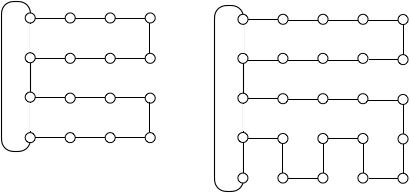
\includegraphics[scale=0.6]{FiguresGraph/HamiltonTorus}
       \caption{Principle for building hamiltonian cycles (even-even and odd-odd).}
  \label{fig:HamiltonTorus}
\end{center}
\end{figure}
\medskip

\noindent {\bf (d)}
One can craft a Hamiltonian cycle in $\q_n$ by
generating an {\it order-$n$ binary reflected Gray code}---so named
for its inventor, Bell Laboratories researcher \index{Gray, Frank}
Frank Gray; see \cite{PetersonW81}.  \index{Gray code} \index{binary
  reflected Gray code} Such a ``code'' is a cyclic enumeration of all
$2^n$ binary strings of length $n$ having the property that cyclically
adjacent \index{strings!cyclically adjacent} strings differ in only
one bit-position.  Length-$n$ strings $x_i$ and $x_j$ are {\it
  cyclically adjacent} in the Gray code $\langle x_0, \ x_1, \ldots,
x_{2^n-1} \rangle$ if $j = i+1 \bmod 2^n$.

\noindent
It is computationally easy to generate an order-$n$ Gray code from an
order-$(n-1)$ Gray code, as follows.

We note first that the order-$1$ code is the sequence $\langle 0, 1
\rangle$.

Inductively, to generate the order-$(k+1)$ Gray code from the
order-$k$ code:
\begin{itemize}
\item
Concatenate the order-$k$ code with a {\em reversed} copy of itself.
(It is the code-sequence that is reversed, not the individual strings.
For instance, as we go from the order-$2$ code $\langle x_0, \ x_1,
\ x_2, \ x_3 \rangle$ to the order-$3$ code, we concatenate that
sequence with $\langle x_3, \ x_2, \ x_1, \ x_0 \rangle$.)
\item
Augment each length-$k$ string in one copy of the order-$k$ Gray code
to length $(k+1)$ by prepending a $0$ to each string; and, augment
each length-$k$ string in the other (reversed) copy of the order-$k$
Gray code to length $(k+1)$ by prepending a $1$ to each string.
\end{itemize}
The following table illustrates the first few steps of this process.
\begin{equation}
\label{eq:gray-code}
 {\small
\begin{array}{|c|c|c|c|}
\hline
\mbox{Order } \ 1
  & \mbox{Order } \ 2
  & \mbox{Order } \ 3
  & \mbox{Order } \ 4 \\
\hline
0   & 00   & 000  &  0000 \\ 
1   & 01   & 001  &  0001 \\
    & 11   & 011  &  0011 \\
    & 10   & 010  &  0010 \\
    &      & 110  &  0110 \\
    &      & 111  &  0111 \\
    &      & 101  &  0101 \\
    &      & 100  &  0100 \\
    &      &      &  1100 \\  
    &      &      &  1101 \\  
    &      &      &  1111 \\  
    &      &      &  1110 \\  
    &      &      &  1010 \\  
    &      &      &  1011 \\  
    &      &      &  1001 \\  
    &      &      &  1000 \\  
\hline
\end{array} }
\end{equation}

We now sketch a proof that for each index $n \in \N^+$, the order-$n$
Gray code sequence specifies a Hamiltonian cycle in $\q_n$; exercises
will give the reader the opportunity to fill in details.  We verify
the following two assertions in turn:
\begin{enumerate}
\item
{\it The order-$n$ Gray code contains all $2^n$ length-$n$ binary
  strings.}
\item
{\it Every pair of cyclically adjacent strings in the order-$n$ Gray
  code differ in a single bit-position.}
\end{enumerate}

(1) We sketch the induction.  When $n=1$, the Gray code consists of
the two distinct strings $0$ and $1$.  Assume that the assertion holds
for $n=k$.  The order-$(k+1)$ code is obtained by taking two copies of
the order-$k$ code and prepending $0$ to the strings in one copy and
$1$ to the strings in the other copy.  The $2^k$ distinct binary
strings from the order-$k$ code thereby produce $2^{k+1}$ distinct
binary strings in the order-$(k+1)$ code.

(2) We distinguish three situations.  Let the adjacent strings be
string $x$, which appears in position $i$ of the code, and string $y$,
which appears in position $i+1 \bmod 2^n$ of the code.
  \begin{itemize}
  \item
Say that $i = 2^n-1$.  In this case $x$ is the last string in the
code, and $y$ is the first string.  By the ``refective'' nature of the
construction of the code, we know that $x = 1z$ and $y = 0z$ for some
length-$(n-1)$ binary string $z$.  Strings $x$ and $y$ therefore
differ in precisely one bit-position, namely, bit-position $0$.

  \item
Precisely the same argument shows that when $i = 2^{n-1} -1$, strings
$x$ and $y$ again differ precisely in bit-position $0$.

  \item
In all other cases, namely, when $i \in \{0,1, \ldots, 2^n-1\}
\setminus \{2^{n-1} -1, 2^n-1\}$, strings $x$ and $y$ share the same
first bit-position.  In fact, for some bit $\beta \in \{0,1\}$, $x =
\beta u$ and $y = \beta v$ for length-$(n-1)$ binary strings $u$ and
$v$ which are cyclically adjacent in the order-$(n-1)$ Gray code.  By
an inductive argument, $u$ and $v$ differ in precisely one
bit-position---which means that $x$ and $y$ also differ in precisely
one bit-position.
  \end{itemize}
  The previous analysis is summarized in Fig.~\ref{fig:HamiltonHypercude}.
  \begin{figure}[hbt]
\begin{center}
       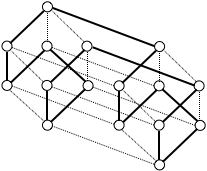
\includegraphics[scale=0.6]{FiguresGraph/HamiltonHypercube}
       \caption{Hamiltonian cycle in Hypercube using reflected Gray codes.}
  \label{fig:HamiltonHypercude}
\end{center}
\end{figure}


\noindent {\bf (e)}
By Proposition~\ref{thm:deBruin-linegraph}, each de Bruijn network
$\d_n$ is the line-digraph of the next bigger de Bruijn network,
$\d_{n+1}$.  Therefore, by definition of ``line (di)graph'', the fact
that $\d_n$ is (directed)-Eulerian
(Corollary~\ref{thm:deBruijn-Eulerian}) means that $\d_{n+1}$ is
(directed)-Hamiltonian.  \qed
\end{proof}


\subsubsection{Testing general graphs for Hamiltonianicity}
\label{sec:Hamiltonian-unweighted}

The techniques we use in Subsection~{\small\sf B} to investigate the
Hamiltonianicity of our ``named'' graphs exploit the detailed
structures of the individual graphs.  Thus, we cannot expect the proof
of Proposition~\ref{thm:named-graph-Hamiltonian} to suggest avenues
for determining whether an arbitrary given graph is Hamiltonian.  In
fact, quite sophisticated results proved in the early 1970s make a
strong mathematical argument that no set of case studies is likely to
have a major impact on the problem of testing general graphs for
Hamiltonianicity.  This is because, in common with the Satisfibility
problem {\sf 3SAT} of Section~\ref{sec:Satisfiability}, the
Hamiltonianicity-detection problem is {\sf NP}-complete.  We repeat
from our discussion in Section~\ref{sec:Satisfiability} that the
details of the theory of {\sf NP}-completeness are beyond the scope of
this text, but we do want the reader to recognize the following.
\begin{description}
\item
{\it The problem of deciding, given a graph $\g$ that is presented via
  a list of nodes and a list of edges, whether $\g$ admits a
  Hamiltonian path or a Hamiltonian cycle is {\sf NP}-complete.}
\end{description}


%%%%%%%%%%%%%%%%%%%%%%%%%%%%%%%%%%%

\section{$\oplus$ Pointers to Advanced Topics}
\label{sec:advanced-topics}

%**PROVIDE SOME REFERENCES

We conclude this chapter by mentioning a variety of topics that are
typically not covered---at least in depth---early in the curriculum,
but that are important enough that the reader should at least be aware
of them.  The topics we mention are motivated by virtually every
computational area that benefits from graph-theoretic models.  We have
tried to present each topic we touch on at a level of discourse that
will prepare the interested reader to delve more deeply into the
material, yet at a level of informality that will make the material
accessible to the more casual reader.  We thus strive for an intuitive
presentation that will not lead any reader astray.

The problem that we discuss in Section~\ref{sec:Relate-CS-Math-Probs}
illustrates how the {\em dynamic} models in the field of
algorithmics---``dynamic'' in the sense that they {\em do}
something---and the {\em structural} models provided by graph theory
can often provide beneficial illumination of one another.

Section~\ref{sec:graph-decompose} \index{graphs!graph separators}
\index{graphs!graph decomposition} focuses on the myriad computations
on graph that can be accomplished efficiently via recursive algorithms
that decompose, then reassemble, the graphs that they work on.

Section~\ref{sec:graph-evolve} \index{graphs!evolving graphs}
introduces the increasingly important topic of graphs whose structure
changes dynamically over time.  One timely instance of this dynamic
evolution is the connectivity graph of the Internet.

Section~\ref{sec:hypergraphs} \index{graphs!hypergraphs}
\index{hypergraphs} introduces {\it hypergraphs}, a generalization of
graphs that allows multi-entity relationships, in contrast to the
binary relationships mandated by graphs' two-element edges.
Hypergraph-based models find application in areas as diverse as:
\begin{itemize}
\item
{\it social networks:} Hyperedges can describe, e.g., collaboration
and collusion.
\item
{\it electronic networks:} Hyperedges can enable the design of
equi-potential nodes in voltage-driven technologies such as {\it
  VLSI}.
\item
{\it communication networks:} Hyperedges can model bus-oriented
communication.
\end{itemize}

\subsection{Hamiltonianicity in Weighted Graphs: the TSP}
\label{sec:TSP}
\index{Traveling Salesman Problem}

In Section~\ref{sec:Hamiltonian-unweighted}, we suggested how daunting
it is computationally to determine whether an unweighted graph admits
a Hamiltonian cycle.  There is an important, practically significant,
analogue of this problem for edge-weighted graphs, which has
traditionally been known as the {\it Traveling Salesman Problem}; we
shall use the modern abbreviation {\it TSP}.
\index{Traveling Salesman Problem}
\index{TSP: the Traveling Salesman Problem}
The TSP is a classical problem in Operations Research, whose familiar
name arises from the following story.
\index{Traveling Salesman Problem!origin of the name}

We consider a saleswoman who wants to make a call on all of her $n$
clients, who live in the $n$ cities, $C_1, C_2, \ldots, C_n$.  In
order to minimize the {\it cost} of her tour, she studies the
$\displaystyle {n \choose 2}$ real numbers $\{c_{i,j} \ | \ 1 \leq i,j
\leq n\}$, where each $c_{i,j}$ is the {\it cost} of traveling between
cities $C_i$ and $C_j$ (in either direction).  
\bigskip

\noindent \fbox{
\begin{minipage}{0.95\textwidth}
We are purposely vague about the meaning of the word ``cost'' here.
The costs represented by the unknowns $c_{i,j}$ could be intercity
driving distances or inter-region travel times or international
airfares.  Instances of the TSP can be formulated with {\em any}
notion of cost that can be represented by positive real numbers.

\smallskip

The importance of being vague is that, in particular, {\em none of
  these costs is assumed to obey any of the laws that one commonly
  associates with the distances we encounter in our daily lives}.  The
{\it triangle inequality} is a prime example of such a law.
\index{triangle inequality} Intuitively, this law insists that the
distance between any two cities is never decreased by placing an
intermediate stopover city between them.  It is a discretization of
the geometric postulate, {\em A straight line is the shortest distance
  between two points.}  Cost measures that obey the triangle
inequality are termed {\it Euclidean} \index{Euclidean distance
  measure} \index{Euclid} because the distances studied in Euclidean
geometry are assumed to obey this law.

\smallskip

Some people like to think of general intercity costs as
airfares---which clearly obey no immutable laws.)
\end{minipage}
}
\bigskip

The saleswoman's objective is to schedule the order of visiting her
clients' $n$ cities in the most economical way.  Formally, the
challenge of the TSP is to discover a minimum-cost tour of all $n$
cities.  Such a tour would be a cycle of the form
\[ C_{i_1} \ - \ C_{i_2} \ - \cdots - \ C_{i_n} \ - \ C_{i_1} \]
such that:
\begin{itemize}
\item
all $n$ cities appear in the tour precisely once;
\item
no tour has cost smaller than the cost
\[ c_{i_1,i_2} \ + \ c_{i_2, i_3} \ + \cdots + \  
c_{i_{n-1}, i_n} \ + \ c_{i_n, i_1} \]
of the indicated tour.
\end{itemize}
The main connection of the TSP to the current chapter is twofold.
\begin{enumerate}
\item
The TSP can be represented as a weighted analogue of the problem of
detecting Hamiltonian cycles.  Within this representation, the TSP's
$n$ cities are depicted as an instance of the complete graph $\k_n$,
and its intercity costs are real-number weights on the edges of
$\k_n$.  We describe this representation via the following informal,
but precise, encoding of a graph $\g$ as an instance of the TSP.
  \begin{itemize}
  \item
Each node of $\g$ becomes a ``city'' that must be visited.
  \item
For each pair of cities/nodes $A$ and $B$:
\[ \mbox{\sc cost}(A,B) \ = \ \left\{
\begin{array}{ccl}
1 & & \mbox{if there is an edge between $A$ and $B$ in $\g$} \\
\infty & & \mbox{if there is no edge between $A$ and $B$ in $\g$} \\
       & & \mbox{\small\sf (if the idea of ``infinite'' cost bothers
  you, then} \\
       & & \mbox{\small\sf make this some ridiculousy large number)}
\end{array}
\right.
\]
  \end{itemize}

\item
The TSP is computationally ``no easier'' than the
Hamiltonianicity-detection problem, in a very strong sense.  By
definition, the target of the TSP is a tour of minimum {\em overall
  cost}, as measured by the sum of the costs of the edges traversed in
the tour.  But, of course, {\em every} tour has some cost, according
to this measure.  The computational difficulty of the TSP is suggested
by the following result, which we state without proof.
\end{enumerate}

\begin{prop}[\cite{GareyJ79}]
\label{thm:Approx-TSP-NPC}
For any fixed positive constant $\kappa$, the problem of finding a
tour for an instance of the TSP that is within a factor of $\kappa$ of
minimal is an {\sf NP}-complete problem.
\end{prop}


The fact that TSP is a computationally complex problem is not very
surprising, because the TSP can be framed in a way that encompasses a
form of the Hamiltonianicity-detection problem.
What {\em is} surprising, though, is that if we restrict attention to
{\em Euclidean} instances of the TSP---i.e., instances whose ``costs''
measure Euclidean \index{Euclidean TSP problem} distances---say,
driving distances---then there exists a rather efficient algorithm
that solves such instances of the TSP {\em approximately} optimally,
\index{Traveling Salesman Problem!approximately optimal solution}
\index{TSP: the Traveling Salesman Problem!approximately optimal solution} 
in the sense of Proposition~\ref{thm:Approx-TSP-NPC}.  That is, there
exists a fixed constant $\kappa > 0$ such that, for each Euclidean
instance $\i$ of the TSP, if an {\em optimal}---i.e., {\em
  cost-minimal}---tour for instance $\i$ has cost $c^\star$, then the
cost of the tour discovered by the algorithm is no larger than $\kappa
\cdot c^\star$.  The algorithm that achieves this approximation is
named for its inventor, Nicos Christofides.
\index{Christofides, Nicos}

\ignore{*********
It corresponds to determine a minimal Hamiltonian cycle in a weighted
complete graphs $K_n$.  Obviously, $K_n$ is Hamiltonian (it exists
$n!$ such Hamiltonian paths), thus, the question here is to determine
the minimum one.

  Of course, she must go in every city and her objective is to
minimize the total distance done in the tour.  The only information
she has is the list of the cities and a map with all inter-cities
distances.  We assume a \textit{Euclidian distance} (for instance the
weights correspond to number of kilometers between two cities).  This
property means that the straight line is always the minimum distance,
or in other words that the distance between two vertices/cities is
larger if the path is going through any other vertex.
%More formally, the input of the problem is a weighted matrix with an infinite weight on the diagonal.
\bigskip
*****************}

\begin{prop}[\cite{Christofides76}]
There exists an algorithm for the Euclidean TSP that produces
approximately optimal tours, specifically, tours whose costs are no
greater than $1.5$ times the cost of an optimal tour.
\end{prop}

Proving this result is the domain of an algorithms text such as
\cite{CLRS}.  We remark only that the algorithm combines a number of
classical computational problems that admit efficient solutions:
minimum-weight spanning trees, preorder walks within trees, and
minimum-weight perfect matchings.

\ignore{***************
We construct an efficient solution for the Euclidean TSP, which is
known as {\it the Christofides algorithm}, \index{Christofides algorithm} 
after its inventor, Nicos Christofides.
\index{Christofides, Nicos}
\cite{Christofides76}

The following table, and Fig.~\ref{fig:perfectMatchingInitial}, depict
an instance of the Euclidian TSP with $n=7$ cities.
\[
\begin{array}{|c||c|c|c|c|c|c|c|}
\mbox{\bf City} & \multicolumn{6}{c}{\mbox{\bf Inter-City Costs}} \\
\hline
C_1 & 0 & c_{1,2} & c_{1,3} & c_{1,4} & c_{1,5} & c_{1,6} & c_{1,7} \\
\hline
C_2 & c_{2,1} & 0 & c_{2,3} & c_{2,4} & c_{2,5} & c_{2,6} & c_{2,7} \\
\hline
C_3 & c_{3,1} & c_{3,2} & 0 & c_{3,4} & c_{3,5} & c_{3,6} & c_{3,7} \\
\hline
C_4 & c_{4,1} & c_{4,2} & c_{4,3} & 0 & c_{4,5} & c_{4,6} & c_{4,7} \\
\hline
C_5 & c_{5,1} & c_{5,2} & c_{5,3} & c_{5,4} & 0 & c_{5,6} & c_{5,7} \\
\hline
C_6 & c_{6,1} & c_{6,2} & c_{6,3} & c_{6,4} & c_{6,5} & 0 & c_{6,7} \\
\hline
C_7 & c_{7,1} & c_{7,2} & c_{7,3} & c_{7,4} & c_{7,5} & c_{7,6} & 0 \\
\hline
\end{array}
\]


\begin{figure}[hbt]
\begin{center}
       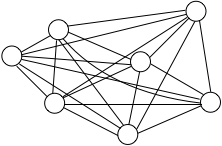
\includegraphics[scale=0.8]{FiguresGraph/christofides1}
\caption{An instance of the Euclidean TSP with $7$ cities, $C_1$,
  $C_2$, $C_3$, $C_4$, $C_5$, $C_6$, $C_7$, and intercity costs
  $\{c_{i,j} \ | \ 1 \leq i,j \leq 7\}$.}
              \label{fig:christofidesInitial}
\end{center}
\end{figure}


Let us construct a good solution (not \textit{too far} from the optimal) in polynomial time. 
Let us denote by $\omega_G$ the weight of graph G (i.e. the sum of the weights on its edges). 
The Chritofides algorithm proceeds in three steps. 
\bigskip

\textbf{Step 1.} Determine a minimal weight spanning tree $T^*$. 
%A spanning tree of G is a tree (connected graph with no cycle) with the same set of vertices as G. 
As we recalled in the preliminaries, a minimal weight spanning tree can be determined in polynomial time. 
\bigskip

$\omega_{T^*}$ is a lower bound of the value of the optimal tour $\omega_{H^*}$. 
Indeed, $H^*$ is a cycle, then, removing any edge in $H^*$ leads to a chain, which is a particular spanning tree.
As $T^*$ is the minimal spanning tree, we have:
$\omega_{T^*} \leq \omega_{H^*}$.

\begin{figure}[hbt]
\begin{center}
       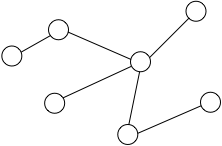
\includegraphics[scale=0.6]{FiguresGraph/christofides2}
       \caption{Construction of an optimal spanning Tree $T^*$.}
              \label{fig:christofidesSpanningTree}
\end{center}
\end{figure}


\textbf{Step 2.} Consider now the set $V_{odd}$ of the vertices of $T^*$ whose degrees are odd. 

We proved in the preliminary properties that the cardinality of $V_{odd}$ is even. 

Let us construct the perfect matching $C^*$ of minimum weight between the vertices in $V_{odd}$. 
Fig.~\ref{fig:AllPerfectMatchings} shows all possible perfect matchings on the previous example, the optimal one (with minimal weight) is represented in bold. 

Fig.~\ref{fig:christofidesPerfectMatching} illustrates the graph obtained by considering the edges of both $T^*$ and $C^*$. 
\begin{figure}[hbt]
\begin{center}
       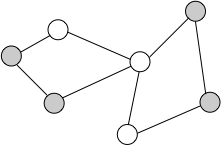
\includegraphics[scale=0.6]{FiguresGraph/christofides3}
       \caption{Adding the optimal perfect matching $C^*$ to the minimal spanning tree $T^*$.}
              \label{fig:christofidesPerfectMatching}
\end{center}
\end{figure}

Let us now determine a lower bound of the optimal tour $H^*$ (represented in Fig.~\ref{fig:perfectMatchingInitial}).

$2 \omega_{C^*}$ is a lower bound of the value of the optimal tour ($\omega_{C^*} \leq \frac{1}{2} \omega_{H^*}$). 
Indeed, consider first the perfect matching $C^*$.
As its vertices belong to $H^*$, $\omega_{C*}$ is lower than the piece of Hamiltonian tour contained between these vertices
because of the euclidian property (see Fig.~\ref{fig:perfectMatchingC*}).
Similarly for the \textit{complementary} perfect matching $C$ (Fig.~\ref{fig:perfectMatchingC}).  
Thus, the weight of the cycle formed by the concatenation of both perfect matchings is lower than the Hamiltonian tour $\omega_{C^* \bigcup C} \leq \omega_{H^*}$.
Moreover, as $C^*$ is the minimum perfect matching, we have $\omega_{C^*} \leq \omega_{C}$, this concludes the proof.


\begin{figure}[hbt]
\begin{center}
       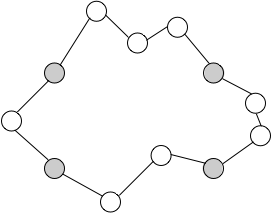
\includegraphics[scale=0.7]{FiguresGraph/perfectmatching1}
       \caption{An optimal Hamiltonian cycle $H^*$.}
              \label{fig:perfectMatchingInitial}
\end{center}
\end{figure}

\begin{figure}[hbt]
\begin{center}
       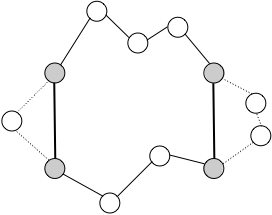
\includegraphics[scale=0.7]{FiguresGraph/perfectmatching2}
       \caption{Perfect matching $C^*$ between the vertices of odd degrees.}
              \label{fig:perfectMatchingC*}
\end{center}
\end{figure}

\begin{figure}[hbt]
\begin{center}
       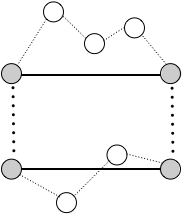
\includegraphics[scale=0.7]{FiguresGraph/perfectmatching3}
       \caption{Cycle $C^* \bigcup C$ (in dashed and bold).}
              \label{fig:perfectMatchingC}
\end{center}
\end{figure}

\bigskip

\textbf{Step 3.} 
All the vertices of $T^* \cup C^*$ have an even degree since we added an edge of $C^*$ to every odd degree vertices of $T^*$. 
We are now going to transform this graph by replacing iteratively the high degree vertices by shortcuts, which decreases the degree until reaching $2$. 

While it exists a vertex of degree greater than 4, we remove two of these consecutive edges and replace them by the opposite edge of this triangle 
without disconnecting the graph. There are $2k$ ways to remove $2$ edges and replace them by the triangle edge. Some of them disconnect the graph
and thus, must be avoided. 
Fig.~\ref{fig:christofidesFinalStep1} shows such a transformation on the previous example, 
Fig.~\ref{fig:christofidesFinalStep2} shows a valid transformation.

\begin{figure}[hbt]
\begin{center}
       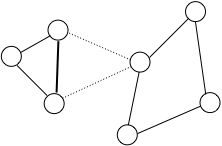
\includegraphics[scale=0.6]{FiguresGraph/christofides4}
       \caption{Reduction of the degree in $T^* \bigcup C^*$, disconnected solution.}
              \label{fig:christofidesFinalStep1}
\end{center}
\end{figure}

\begin{figure}[hbt]
\begin{center}
       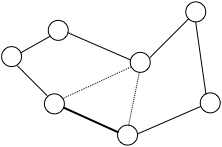
\includegraphics[scale=0.6]{FiguresGraph/christofides5}
       \caption{Reduction of the degree in $T^* \bigcup C^*$, connected solution.}
       \label{fig:christofidesFinalStep2}
\end{center}
\end{figure}

This process leads to a feasible tour. 
Such transformations do not increase the total weight.

Finally, 
as $\omega_{T^*} \leq \omega_{H^*}$ and $\omega_{C^*} \leq 1/2 \omega_{H^*}$,
we deduce that the value of such a tour is lower than $3/2 \omega_{H^*}$.
\qed
\end{proof}
*****************}


\subsection{Relating Computational and Mathematical Problems}
\label{sec:Relate-CS-Math-Probs}

This 

\ignore{*******************

\subsubsection{The Route Inspection/ Chinese Postman Problem}
\label{sec:chinesePostman}

**HERE

After solving the preceding ``pure'' version of the Eulerian-tour
problem---which seeks a tour of a graph which crosses each edge
precisely once---we discuss an extension of this problem which allows
us to augment a graph $\g$ by adding multiple edges between the same
two nodes.  (Terminologically, we thereby convert $\g$ to a {\it
  multi-graph} \index{multi-graph} \index{graphs!multi-graph}
consisting of nodes and {\it multi-edges}.) \index{multi-edge} Not
obviously, adding multi-edges can often convert a graph $\g$ that does
not admit an Eulerian cycle into a multi-graph that does admit an
Eulerian cycle.  The problem of finding the {\em smallest} such
augmentation of $\g$---i.e., of adding the fewest multi-edges---is
called the \index{Route Inspection Problem} {\it Route Inspection
  Problem}; it is also often called the {\it Chinese Postman Problem},
\index{Chinese Postman Problem} in honor of its inventor, the Chinese
mathematician Kwan Mei-Ko \index{Kwan Mei-Ko} \cite{Kwan60}.



This section is devoted to studying the {\it Route Inspection
  Problem}, \index{Route Inspection Problem} also known as the {\it
  Chinese Postman Problem}, \index{Chinese Postman Problem} in honor
of its inventor, the Chinese mathematician Kwan Mei-Ko \index{Kwan
  Mei-Ko} \cite{Kwan60}.  This problem seeks to add as few multi-edges
\index{graphs!multi-graph!multi-edge} as possible to a graph $\g$ in
order to render $\g$ Eulerian.  (A {\it multi-graph} is ``almost'' an
undirected graph.  It differs from a true graph because of the
possible presence of multiple multi-edges that connect the same two
nodes.)

**HERE


We know from Proposition~\ref{thm:eulerian-cycle} that if all of
$\g$'s nodes have even node-degrees, then---{\em and only then}---$\g$
admits an Eulerian cycle.  Therefore, in this case, {\em zero}
multi-edges need be added to $\g$ to render it Eulerian.  

Let us now present the more general problem of determining a cycle that contains all the edges in any graph, in particular when
there exist some odd vertices. From the previous section, we know that there is no Eulerian cycle in this case and thus, 
any feasible solution should duplicate some edges.
The problem is to duplicate the minimum.
This problem is known as the {\it chinese postman} and it is described below (in a french equivalent version).

A postman moved recently from Grenoble to a small village in the country side. 
He asked himself how to organize his daily tour by bike for distributing the letters in the shortest possible time. 
The director of the post office gives him the map and 
fortunately, the postman had some old souvenir of previous lectures in Graph Theory.  
The tour starts from the post office and of course, the postman has to go through every roads for distributing the letters before coming back
to his office.
The underlying graph is $G=(V,E)$ where $V$ is the (finite) set of cross points and $E$ is the set of the links between the cross roads
weighted by the distances.  

Fig.~\ref{fig:EulerianInitial} presents an example of the chinese postman problem. 
\begin{figure}[hbt]
\begin{center}
       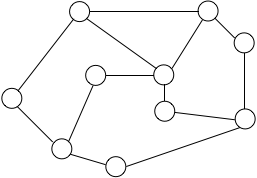
\includegraphics[scale=0.6]{FiguresGraph/EulerienInitial}
       \caption{An instance of the Chinese postman with $10$ cross-nodes.}
              \label{fig:EulerianInitial}
\end{center}
\end{figure}

\bigskip

This problem can be formulated mathematically in term of Eulerian
cycles.  Intuitively, the basic idea is to duplicate some edges that
are carefully chosen in order to use the previous construction of an
Eulerian tour of Section~\ref{sec:EulerianCycle} that will help the
postman to determine the optimal tour (of minimal length) using some
simple mathematical properties.
\bigskip

First, we know that there is an even number of odd vertices.
Considering the previous instance of the postman problem, there are $4$ such vertices (represented in grey in Fig.~\ref{fig:EulerianVodd}).

\begin{figure}[hbt]
\begin{center}
       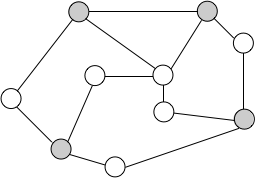
\includegraphics[scale=0.6]{FiguresGraph/EulerienVodd}
       \caption{The $4$ vertices with an odd degree in the previous instance.}
              \label{fig:EulerianVodd}
\end{center}
\end{figure}
\bigskip

As there exists a path between any pair of vertices of odd degree in $V_{odd}$,
we consider the complete graph whose vertices are the odd degree vertices weighting the edges with the shortest paths (denoted by $K_{odd}$).
As we mentioned in the preliminary properties, computing the shortest paths is a classical problem, which can be solved in polynomial time. 

\begin{figure}[hbt]
\begin{center}
       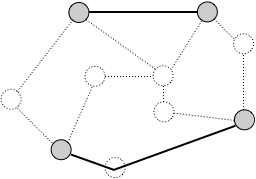
\includegraphics[scale=0.6]{FiguresGraph/EulerienPerfectMatching}
       \caption{The minimum weight perfect matching labelled by the shortest distances between the vertices of $V_{odd}$.}
              \label{fig:Eulerianperfectmatching}
\end{center}
\end{figure}
\bigskip

Then, it is possible to do the correspondence between the optimal solution of the postman problem and a perfect matching of minimal weight in $K_{odd}$
%Recall that a matching is a set of edges without common vertices. It is perfect if it has the maximum number of edges. 
by duplicating the edges of the minimal perfect matching.

\begin{figure}[hbt]
\begin{center}
       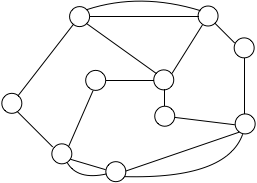
\includegraphics[scale=0.6]{FiguresGraph/EulerienFinal}
       \caption{Final step: adding the edges of the minimum perfect matching.}
              \label{fig:EulerianFinal}
\end{center}
\end{figure}

The main steps of the algorithm for determining the optimal tour are the following:

\begin{itemize}
\item Consider the complete graph with the odd vertices and compute its weight by the shortest paths.
Compute a perfect matching of minimal weight between these vertices. 
\item Duplicate all the edges along the paths of this matching.
\item Determine an Eulerian tour in this new graph with even degrees.
\end{itemize}

The optimality of this algorithm comes from the fact that the duplicated edges are the minimum possible ones.
% This is straightforward for two odd vertices.
Finally, all the vertices of the new graph are even since the degree of the odd vertices in $G$ is augmented by $1$
(extremities of the paths) and the other even vertices which are intermediate vertices of the paths remain even. 

\medskip

This short discussion is a good segu\'{e} to the material in the next
section, which leds valuable perspective on our brief study of
Hamiltonian paths and cycles---and, indeed, on the computational
implications of that work.
*************************}

\subsection{Graph Decomposition}
\label{sec:graph-decompose}
\index{graphs!decomposition}
\index{graphs!bisector}
\index{graphs!separator}

The reader will certainly have noted that some ``named'' graphs are,
intuitively, more tightly interconnected than others.  From a purely
intellectual vantage point, it would be of interest to be able to
quantify the tightness of interconnection.  Among the various measures
that have been proposed, one stands out for its myriad algorithmic
implications: the notion of {\it graph separator}.  In fact, this
notion appears in the literature in several flavors.  An $n$-node,
$e$-edge graph $\g$ has:
\begin{itemize}
\item
an {\it $\alpha$-edge separator} of size $k$, 
\index{graphs!$\alpha$-edge separator of size $k$} where $\alpha$ is a
real number with $\alpha \leq 1/2$ and $k$ is an integer with $k < n$,
precisely if:

\smallskip

one can partition $\g$ into two disjoint (not-necessarily connected)
subgraphs, each having $\leq \alpha n$ nodes, by removing $\leq k$
edges from $\g$.

\item
a {\it $\alpha$-node separator} of size $\ell$,
\index{graphs!$\alpha$-node separator of size $\ell$}
where $\alpha$ is a real number with $\alpha \leq 1/2$ and $\ell$ is
an integer with $k < e$, precisely if:

\smallskip

one can partition $\g$ into two disjoint (not-necessarily connected)
subgraphs, each having $\leq \alpha n$ nodes, by removing $\leq \ell$
nodes from $\g$.
\end{itemize}
We replace the term ``separator'' with the term {\em ``bisector''} 
\index{graphs!edge bisector} \index{graphs!node bisector}
if both subgraphs after a separation operation have $\leq \lfloor
\frac{1}{2} n \rfloor$ nodes.

\medskip

Commonalities and differences in inherent separator sizes are often
not visually obvious.  For illustration, referring to the ``named''
graphs of Section~\ref{sec:graphs-important-families}:
\begin{itemize}
\item
It is certainly obvious that cycles are easier to bisect than cliques,
as measured by either edge or node bisectors.
\item
It is far less clear that de Bruijn networks and hypercubes are
roughly equal in ease to bisect, as measured by node bisectors.
\end{itemize}
But similar separation behavior has very important algorithmic
consequences.  For instance, the closeness in separation
characteristics between de Bruijn networks and hypercubes manifests
itself in a large range of algorithmic applications.  The range of
such applications is hinted at by sources that study the algorithmics
of laying out VLSI circuits (see, e.g., \cite{Leiserson85}) and
sources that study the ability of a network's interconnections to host
a range of communication patterns that enable efficient parallel
computation and communication (see, e.g.,
\cite{AnnexsteinBR90,Leiserson85,Ullman84}).


\medskip

There is a large literature that develops the algorithmics of finding
small separators for significant families of graphs.  An early star in
the firmament of such studies is the discovery in \cite{LiptonT79} of
a $1/3$-node separator of size $\sqrt{8n}$ for $n$-node planar graphs.
The dual problem of finding lower bounds on the sizes of graph
separators is a bit sparser but, of course, no less significant.  The
reader can find a comprehensive exposition on the theory of graph
separators in \cite{RosenbergH01}, including both the mathematics that
yields lower bounds on separator sizes and the algorithmics that
yields upper bounds.


\subsection{Graphs with Evolving Structure}
\label{sec:graph-evolve}
\index{graphs!with evolving structure}

Classical problems in the area of graph algorithms will discuss
graphs, especially trees, whose structures evolve over time.  Such
evolution is observed, e.g., in the study of ``classical'' algorithmic
problems such as {\it Minimum Spanning Tree} and {\it Branch and
  Bound}; see, e.g., \cite{CLRS}.  What is certain to be more exciting
to the reader, though, are the ``modern'' topics where one encounters
graphs with evolving structure, such as {\it social networks} and {\it
  inter-networks} (e.g., the {\it Internet of Things}).

For ``classical'' topics, as exemplified by the two we have mentioned,
the mathematics covered in this chapter will provide the reader with
the background necessary to deal with graph evolution.  Indeed, this
evolution emerges as an inevitable concomitant of the algorithmics
that is superimposed upon the traditional structures of graph theory:
the challenge to the reader is to assimilate new algorithmic notions,
not new mathematics.

\index{graphs!with evolving structure!social networks}
\index{graphs!with evolving structure!inter-networks}
In contrast, the ``modern'' topics we have mentioned do require the
reader's assimilating new mathematics.  Dealing successfully with the
algorithmic issues that arise with social networks and inter-networks
requires the reader to understand the structures of the evolving
graph-oriented systems and how evolution changes these structures.
Among the interesting (and valuable) mathematical questions one can
pose is: When a new node applies to join an evolving network, which
node in the network is the best one to connect to, in order to best
facilitate one's interactions or influence within the community.  The
latter topic leads, e.g., to the study of {\em power-law} networks.
\index{graphs!with evolving structure!social networks!power-law networks}
\index{graphs!with power-law degreegrowth patterns}
\bigskip

\noindent \fbox{
\begin{minipage}{0.95\textwidth}
An evolving network is said to {\it obey a power law} if there exists
a real number $\gamma >0$ such that, for sufficiently large values of
the integer parameter $k$, the fraction of nodes in the network having
degree $k$ is proportional to $k^{-\gamma}$.
\end{minipage}
}
\bigskip

Little of the abstract work on power-law networks would likely be
studied in depth in any early course; indeed, the structure of these
networks is not yet well understood even in advanced settings.
Attempts to understand power laws with rigor have given rise to a
number of competing, rather sophisticated, abstract models---see,
e.g., \cite{AielloCL00,BarabasiA99,Bollobas85,ChenCGJSW}---and
numerous studies have attempted to understand the specific situations
wherein the abstract models reflect reality more or less
faithfully---see, e.g.,
\cite{BuT02,FaloutsosFF99,JaiswalRT04,TangmunarunkitGJSW02,ZeguraCD97}.


\subsection{Hypergraphs}
\label{sec:hypergraphs}
\index{graphs!generalization to hypergraphs}
\index{hypergraphs}

A large variety of modern computing-related topics benefit from the
structure inherent in graph-theoretic models but do not comfortably
conform to the {\em binary} relationships imposed by graphs' having
{\em two} nodes per edge.  A model that retains the structure of
graph-theoretic models without the binary constraint is the
generalization of graphs called {\em hypergraphs}.  A hypergraph has
nodes that play exactly the same role as with graphs, but in place of
a graph's binary edges, a hypergraph has {\em hyperedges}, each being
a set of nodes whose size is not restricted to $2$.  A rather general
treatment of hypergraphs can be found in the comprehensive
graph-theory text \cite{Berge73}; a specialized article that focuses
on some of the topics of this chapter, such as node-coloring, is
\cite{Lovasz73}.  Because of their inherent complexity, hypergraphs as
graph-theoretic objects are usually relegated to advanced courses.
However, the literature contains many studies of hypergraphs that are
``fine-tuned'' for specific computing-related application areas, and
many of these should be accessible without extensive mathematical
background.  Sample  computing-related application areas that benefit
from hypergraph-oriented models include the following.
\begin{itemize}
\item
Bus-connected parallel communication has been part of digital computer
\index{hypergraphs!modeling bus-connected communication} design since
its earliest days.  The informal picture of such a system is that
there are communication channels that multiple agents can retrieve
message from and post messages to.  In hypergraph-oriented terms: the
nodes/communicating agents aggregate into groups/hyperedges.  Each
group's agents share ``read/write'' access to a specific channel.  A
specialized genre of hypergraph that was invented to study the
described scenario is the {\it interval hypergraph}
\index{hypergraphs!interval hyergraphs} model developed in
\cite{Rosenberg89a}.

\item
Modern electronic circuits are implemented using integrated circuit
\index{hypergraphs!modeling integrated circuits} technology,
specifically, {\em VLSI: Very Large Scale Integrated circuitry}; see,
e.g., \cite{Mead-Conway}.  These technologies tend to be
voltage-driven, rather than current-driven.  Accordingly, much of the
attention when designing circuits centers on the coordination of
equi-potential points in a network, rather than on point-to-point
transmission of signals.  Hypercubes are tailor-made for such
technologies.  A crucially important issue that arises because of the
design strengths and weaknesses of  VLSI technology is {\it fault
  tolerance}---how to cope with the inevitable faulty transistors in
massive VLSI systems.  Even mathematically quite-accessible ideas can
provide provocative ideas about this important topics; see, e.g.,
\cite{Rosenberg85a}

\item
Social networks have become so prevalent in society that no one will
be surprised to learn that many approaches to modeling the networks'
interconnectivity have been studied.  In
Section~\ref{sec:graph-evolve}, we discussed an interconnectivity
model based on evolving graphs and clustering within such graphs.
More recently, hypergraph-based models
\index{hypergraphs!modeling interconnectivity in social networks}
have also been proposed; see, e.g., \cite{Amatoetal17,LiuBV10}.
\end{itemize}





